% !TeX spellcheck = en_GB
% !TeX encoding = UTF-8
% !TeX program = xelatex
% The TDK starter pack: how we work, how a TDK paper comes together, and how to use this
% template. A separate document from the paper (thesis.tex); in Overleaf, choose it under
% Menu > Main document to compile it.
\documentclass[12pt,a4paper,oneside]{report}

% thanks to http://tex.stackexchange.com/a/47579/71109
\usepackage{ifxetex}
\usepackage{ifluatex}
\newif\ifxetexorluatex % a new conditional starts as false
\ifnum 0\ifxetex 1\fi\ifluatex 1\fi>0
   \xetexorluatextrue
\fi

\ifxetexorluatex
  \usepackage{fontspec}
\else
  \usepackage[T1]{fontenc}
  \usepackage[utf8]{inputenc}
  \usepackage[lighttt]{lmodern}
  % Latin Modern Mono has no italic; use slanted (italic comments in code listings).
  {\ttfamily}\DeclareFontShape{T1}{lmtt}{m}{it}{<->ssub*lmtt/m/sl}{} % \ttfamily loads the family first
\fi

\usepackage[english,magyar]{babel} % Alapértelmezés szerint utoljára definiált nyelv lesz aktív, de később külön beállítjuk az aktív nyelvet.

%--------------------------------------------------------------------------------------
% Math and theorems
%--------------------------------------------------------------------------------------
\usepackage{amsfonts,amsmath,amssymb} % Mathematical symbols.
\usepackage[amsmath,thmmarks]{ntheorem} % Theorem-like environments. Do not load amsthm next to it.

%--------------------------------------------------------------------------------------
% Page layout and typography
%--------------------------------------------------------------------------------------
\usepackage{anysize}
\usepackage{setspace} % For setting line spacing
\usepackage{emptypage} % No page number on empty pages.
\usepackage{microtype}
\usepackage{xspace}
\usepackage[normalem]{ulem} % \uline, \sout; normalem keeps \emph italic.
\usepackage{lineno} % \linenumbers for review drafts.

%--------------------------------------------------------------------------------------
% Colors, figures, diagrams
%--------------------------------------------------------------------------------------
\usepackage[table]{xcolor} % Load before tikz, todonotes and tcolorbox so the options stick.
\usepackage{graphicx}
\usepackage[hang]{caption}
\usepackage{subcaption}
\usepackage{wrapfig}
\usepackage{rotating}
\usepackage{placeins} % \FloatBarrier

% SVG figures: \includesvg[width=\linewidth]{figures/foo}. Needs shell escape and Inkscape,
% both available on Overleaf. Locally run the compiler with -shell-escape.
% svg loads the transparent package, which works only with pdfLaTeX and warns otherwise.
% With inkscapelatex=false nothing calls it, so XeLaTeX and LuaLaTeX skip it.
\ifxetexorluatex\expandafter\def\csname ver@transparent.sty\endcsname{2019/11/29 v1.4 (skipped: pdfTeX only)}\fi
\usepackage[inkscapearea=drawing,inkscapelatex=false]{svg}

\usepackage{tikz}
\usetikzlibrary{
  arrows.meta, automata, backgrounds, calc, decorations.pathreplacing, fit,
  patterns, positioning, quotes, shadows, shapes.geometric, shapes.misc,
  shapes.multipart, babel}
\usepackage{pgfplots}
\pgfplotsset{compat=1.18}

% Colored boxes. [most] loads skins, breakable, listings, theorems, etc.
\usepackage[most]{tcolorbox}

%--------------------------------------------------------------------------------------
% Tables and lists
%--------------------------------------------------------------------------------------
\usepackage{booktabs} % For publication quality tables for LaTeX
\usepackage{array}
\usepackage{tabularx}
\usepackage{xltabular} % tabularx across pages; loads longtable.
\usepackage{multirow}
\usepackage{makecell}
\usepackage[inline]{enumitem} % enumerate*, itemize* for inline lists.

%--------------------------------------------------------------------------------------
% Code and algorithms
%--------------------------------------------------------------------------------------
\usepackage{listings} % For source code snippets.
\usepackage[newfloat]{minted} % Pygments highlighting; setup in include/code-languages.tex.
\usepackage[autostyle=true]{csquotes} % \enquote{...}. Load after lineno and fvextra (minted).
\usepackage{algorithm}
\usepackage{algpseudocode}
\usepackage{comment}

%--------------------------------------------------------------------------------------
% Notes, acronyms, citations, links
%--------------------------------------------------------------------------------------
% To hide every todo in the submitted version, add `final` to \documentclass (obeyFinal below
% makes todonotes honour it) or `disable` here.
\usepackage[colorinlistoftodos,obeyFinal]{todonotes}

\usepackage{acro} % Acronyms: define them in content/acronyms.tex, use \ac{key}.

% Citations: natbib + BibTeX. \cite{a,b,c} prints [1-3]; \citet{a} prints "Lamport [1]".
\usepackage[numbers,sort&compress]{natbib}
\newif\ifnamedcitations % true when the bibliography style gives \citet the authors (see thesis-en.tex)

\usepackage{fontawesome5}

\usepackage[unicode]{hyperref} % For hyperlinks in the generated document.
\usepackage{bookmark}
\usepackage{orcidlink} % Loads hyperref itself, so it must come after the line above.
\usepackage[nameinlink,noabbrev,capitalise]{cleveref} % \cref{fig:x} -> "Figure 1.1". Keep after hyperref and ntheorem.


\newcommand{\selecthungarian}{
	\selectlanguage{magyar}
	\setlength{\parindent}{2em}
	\setlength{\parskip}{0em}
	\frenchspacing
}

\newcommand{\selectenglish}{
	\selectlanguage{english}
	\setlength{\parindent}{0em}
	\setlength{\parskip}{0.5em}
	\nonfrenchspacing
	\renewcommand{\figureautorefname}{Figure}
	\renewcommand{\tableautorefname}{Table}
	\renewcommand{\partautorefname}{Part}
	\renewcommand{\chapterautorefname}{Chapter}
	\renewcommand{\sectionautorefname}{Section}
	\renewcommand{\subsectionautorefname}{Section}
	\renewcommand{\subsubsectionautorefname}{Section}
}


\newcommand{\vikcim}{TDK starter pack and template guide}
\newcommand{\vikdoktipus}{Guide}
\newcommand{\szerzoMeta}{Martin Farkas, Imre Kocsis}
\newcommand{\exname}{the credential revocation registry} % the running example of the LaTeX chapter

%--------------------------------------------------------------------------------------
% Elnevezések
%--------------------------------------------------------------------------------------
\newcommand{\bme}{Budapest University of Technology and Economics}
\newcommand{\vik}{Faculty of Electrical Engineering and Informatics}

\newcommand{\bmemit}{Department of Measurement and Information Systems}

\newcommand{\keszitette}{Author}
\newcommand{\konzulens}{Advisor}

\newcommand{\bsc}{Bachelor's Thesis}
\newcommand{\msc}{Master's Thesis}
\newcommand{\tdk}{Scientific Students' Association Report}
\newcommand{\bsconlab}{BSc Project Laboratory}
\newcommand{\msconlabi}{MSc Project Laboratory 1}
\newcommand{\msconlabii}{MSc Project Laboratory 2}

\newcommand{\pelda}{Example}
\newcommand{\definicio}{Definition}
\newcommand{\tetel}{Theorem}

\newcommand{\bevezetes}{Introduction}
\newcommand{\koszonetnyilvanitas}{Acknowledgements}
\newcommand{\fuggelek}{Appendix}

% Optional custom titles
%\addto\captionsenglish{%
%\renewcommand*{\listfigurename}{Your list of figures title}
%\renewcommand*{\listtablename}{Your list of tables title}
%\renewcommand*{\bibname}{Your bibliography title}
%}

\newcommand{\szerzo}{\vikszerzoKeresztnev{} \vikszerzoVezeteknev}
\newcommand{\vikkonzulensA}{\vikkonzulensAMegszolitas\vikkonzulensAKeresztnev{} \vikkonzulensAVezeteknev}
\newcommand{\vikkonzulensB}{\vikkonzulensBMegszolitas\vikkonzulensBKeresztnev{} \vikkonzulensBVezeteknev}
\newcommand{\vikkonzulensC}{\vikkonzulensCMegszolitas\vikkonzulensCKeresztnev{} \vikkonzulensCVezeteknev}

\newcommand{\selectthesislanguage}{\selectenglish}

\bibliographystyle{plainnat}
\namedcitationstrue % plainnat knows the authors, so \citet works

\newcommand{\ie}{i.e.\@\xspace}
\newcommand{\Ie}{I.e.\@\xspace}
\newcommand{\eg}{e.g.\@\xspace}
\newcommand{\Eg}{E.g.\@\xspace}
\newcommand{\etal}{et al.\@\xspace}
\newcommand{\etc}{etc.\@\xspace}
\newcommand{\vs}{vs.\@\xspace}
\newcommand{\viz}{viz.\@\xspace} % videlicet
\newcommand{\cf}{cf.\@\xspace} % confer
\newcommand{\Cf}{Cf.\@\xspace}
\newcommand{\wrt}{w.r.t.\@\xspace} % with respect to
\newcommand{\approximately}{approx.\@\xspace}

\newcommand{\appendixnumber}{1}  % a fofejezet-szamlalo az angol ABC 1. betuje (A) lesz

%--------------------------------------------------------------------------------------
% Page layout setup
%--------------------------------------------------------------------------------------
% we need to redefine the pagestyle plain
% another possibility is to use the body of this command without \fancypagestyle
% and use \pagestyle{fancy} but in that case the special pages
% (like the ToC, the References, and the Chapter pages)remain in plane style

\pagestyle{plain}

\setcounter{tocdepth}{3}
%\sectionfont{\large\upshape\bfseries}
\setcounter{secnumdepth}{3}

\sloppy % Margón túllógó sorok tiltása.
\widowpenalty=10000 \clubpenalty=10000 %A fattyú- és árvasorok elkerülése
\def\hyph{-\penalty0\hskip0pt\relax} % Kötőjeles szavak elválasztásának engedélyezése


%--------------------------------------------------------------------------------------
% Setup hyperref package
%--------------------------------------------------------------------------------------
\hypersetup{
    % bookmarks=true,            % show bookmarks bar?
    unicode=true,              % non-Latin characters in Acrobat's bookmarks
    pdftitle={\vikcim},        % title
    pdfauthor={\szerzoMeta},    % author
    pdfsubject={\vikdoktipus}, % subject of the document
    pdfcreator={\szerzoMeta},   % creator of the document
    pdfproducer={},    % producer of the document
    pdfkeywords={},    % list of keywords (separate then by comma)
    pdfnewwindow=true,         % links in new window
    colorlinks=true,           % false: boxed links; true: colored links
    linkcolor=black,           % color of internal links
    citecolor=black,           % color of links to bibliography
    filecolor=black,           % color of file links
    urlcolor=black             % color of external links
}


%--------------------------------------------------------------------------------------
% Set up listings
%--------------------------------------------------------------------------------------
\definecolor{lightgray}{rgb}{0.95,0.95,0.95}
\lstset{
	basicstyle=\scriptsize\ttfamily, % print whole listing small
	keywordstyle=\color{black}\bfseries, % bold black keywords
	identifierstyle=, % nothing happens
	% default behavior: comments in italic, to change use
	% commentstyle=\color{green}, % for e.g. green comments
	stringstyle=\scriptsize,
	showstringspaces=false, % no special string spaces
	aboveskip=3pt,
	belowskip=3pt,
	backgroundcolor=\color{lightgray},
	columns=flexible,
	keepspaces=true,
	escapeinside={(*@}{@*)},
	captionpos=b,
	breaklines=true,
	frame=single,
	float=!ht,
	tabsize=2,
	literate=*
		{á}{{\'a}}1	{é}{{\'e}}1	{í}{{\'i}}1	{ó}{{\'o}}1	{ö}{{\"o}}1	{ő}{{\H{o}}}1	{ú}{{\'u}}1	{ü}{{\"u}}1	{ű}{{\H{u}}}1
		{Á}{{\'A}}1	{É}{{\'E}}1	{Í}{{\'I}}1	{Ó}{{\'O}}1	{Ö}{{\"O}}1	{Ő}{{\H{O}}}1	{Ú}{{\'U}}1	{Ü}{{\"U}}1	{Ű}{{\H{U}}}1
}


%--------------------------------------------------------------------------------------
% Set up theorem-like environments
%--------------------------------------------------------------------------------------
% Using ntheorem package -- see http://www.math.washington.edu/tex-archive/macros/latex/contrib/ntheorem/ntheorem.pdf

\theoremstyle{plain}
\theoremseparator{.}
\newtheorem{example}{\pelda}

\theoremseparator{.}
%\theoremprework{\bigskip\hrule\medskip}
%\theorempostwork{\hrule\bigskip}
\theorembodyfont{\upshape}
\theoremsymbol{{\large \ensuremath{\centerdot}}}
\newtheorem{definition}{\definicio}

\theoremseparator{.}
%\theoremprework{\bigskip\hrule\medskip}
%\theorempostwork{\hrule\bigskip}
\newtheorem{theorem}{\tetel}


%--------------------------------------------------------------------------------------
% Some new commands and declarations
%--------------------------------------------------------------------------------------
\newcommand{\code}[1]{{\upshape\ttfamily\scriptsize\indent #1}}
\newcommand{\doi}[1]{DOI: \href{http://dx.doi.org/\detokenize{#1}}{\raggedright{\texttt{\detokenize{#1}}}}} % A hivatkozások közt így könnyebb DOI-t megadni.

\DeclareMathOperator*{\argmax}{arg\,max}
%\DeclareMathOperator*[1]{\floor}{arg\,max}
\DeclareMathOperator{\sign}{sgn}
\DeclareMathOperator{\rot}{rot}


%--------------------------------------------------------------------------------------
% Setup captions
%--------------------------------------------------------------------------------------
\captionsetup[figure]{
	width=.75\textwidth,
	aboveskip=10pt}

\renewcommand{\captionlabelfont}{\bf}
%\renewcommand{\captionfont}{\footnotesize\it}

%--------------------------------------------------------------------------------------
% Hyphenation exceptions
%--------------------------------------------------------------------------------------
\hyphenation{Shakes-peare Mar-seilles ár-víz-tű-rő tü-kör-fú-ró-gép}


\author{\vikszerzo}
\title{\viktitle}

%--------------------------------------------------------------------------------------
% Todo notes
%--------------------------------------------------------------------------------------
% The page margins are narrow (see \marginsize in thesis.tex), so margin notes get
% squeezed. Prefer \todo[inline]{...} for anything longer than a few words.
\setlength{\marginparwidth}{13mm}
\newcommand{\todoinline}[1]{\todo[inline]{#1}}


%--------------------------------------------------------------------------------------
% Acronyms (acro)
%--------------------------------------------------------------------------------------
\acsetup{
  make-links = true,     % \ac links to the list of acronyms
  list/heading = chapter*,
}
% Declare every acronym here; use \ac{key} in the text (first use expands it),
% \acs{key} for the short form, \acl{key} for the long form, \acp{key} for plural.
% Print the list with \printacronyms (see thesis.tex).
\DeclareAcronym{vc}{
  short = VC,
  long  = verifiable credential,
}
\DeclareAcronym{zkp}{
  short = ZKP,
  long  = zero-knowledge proof,
}



%--------------------------------------------------------------------------------------
% Colored boxes (tcolorbox)
%--------------------------------------------------------------------------------------
% theo: top-ruled box with a detached title, from Bertalan's BPM paper.
% Usage: \begin{tcolorbox}[theo=blue, title={Key insight}] ... \end{tcolorbox}
\tcbset{%
    theo/.style={%
        enhanced,
        breakable = true,
        sharp corners,
        before skip=20pt,
        toprule=1pt, rightrule=0pt, bottomrule=0pt, leftrule=0pt,
        colback=#1!15, colframe=#1!50, coltitle=#1!60!black,
        detach title,
        overlay unbroken and first ={
            \node[minimum width=1cm, anchor=south west, font=\bfseries]
               at (frame.north west) {\tcbtitle};
        }
    }
}

% Ready-made boxes for the common cases. The optional argument is the title.
\newtcolorbox{infobox}[1][]{enhanced, breakable, colback=blue!5, colframe=blue!50!black, fonttitle=\bfseries, title={#1}}
\newtcolorbox{warnbox}[1][]{enhanced, breakable, colback=orange!8, colframe=orange!70!black, fonttitle=\bfseries, title={#1}}
\newtcolorbox{keybox}[1][]{theo=teal, title={#1}}


%--------------------------------------------------------------------------------------
% Cross-references (cleveref)
%--------------------------------------------------------------------------------------
% Write \cref{fig:overview} instead of Figure~\ref{fig:overview}; \Cref at sentence start.
% Names for the ntheorem environments defined above; cleveref knows the standard ones.
\crefname{definition}{Definition}{Definitions}
\crefname{theorem}{Theorem}{Theorems}
\crefname{example}{Example}{Examples}
\crefname{lstlisting}{Listing}{Listings}
\crefname{rq}{RQ}{RQs}

% Research questions: \begin{rqlist} \item\label{rq:scale} ... \end{rqlist}, then \cref{rq:scale}.
\newlist{rqlist}{enumerate}{1}
\setlist[rqlist]{label=\textbf{RQ\arabic*}, ref=\arabic*, leftmargin=*}
\crefalias{rqlisti}{rq}
\creflabelformat{rq}{#2#1#3}


% Room for chapter numbers like "12." in the Hungarian chapters' table-of-contents entries.
\makeatletter\patchcmd{\l@chapter}{1.5em}{2.3em}{}{\PackageWarning{guide}{l@chapter patch failed}}\makeatother

\singlespacing
\marginsize{15mm}{15mm}{15mm}{15mm}

\begin{document}
\pagenumbering{gobble}
\hypersetup{pageanchor=false}
\selectthesislanguage

\begin{titlepage}
  \centering
  
\includegraphics[width=60mm]{figures/bme_logo}\par\vspace{1cm}
  {\large \bme\\\vik\\\bmemit\par}\vspace{4cm}
  {\Huge \vikcim\par}\vspace{1cm}
  {\large Budapest University of Technology and Economics, FTSRG\par}\vspace{2cm}
  {\large \szerzoMeta\par}\vfill
  {\large \the\year\par}
\end{titlepage}

\tableofcontents
\listoftodos
\clearpage
\pagenumbering{arabic}
\hypersetup{pageanchor=true}

\part*{Guide}\addcontentsline{toc}{part}{Guide}
%----------------------------------------------------------------------------
\chapter{Getting started}\label{app:start}
%----------------------------------------------------------------------------
This guide is the starter pack of the FTSRG advisors, Martin Farkas (\href{https://github.com/BlackLight54}{\texttt{BlackLight54}} on GitHub) and Imre Kocsis (\href{https://github.com/imrekocsis}{\texttt{imrekocsis}}): what to do before you write, how a TDK paper comes together, how we work together, and the tools we recommend.
It comes at the end of the paper template, after the appendices. Nothing has to be deleted before you submit: \texttt{reviewer.tex} builds the paper without the guide and without any note (\cref{app:latex:todo}), and that PDF is the one you upload.

The template uses three kinds of notes. \todo[inline]{An orange note is for you: what a part of the paper must contain.}
\advisortodo{A blue note is for us: a draft we still have to confirm, or a link we still have to add.}
\atodo[inline]{A green note, marked A, is our review comment on your paper. Resolve it, then delete it.}

Work through the steps below in order in your first week. Each says who does it.

%----------------------------------------------------------------------------
\section{Share your identifiers}\label{app:start:ids}
\emph{You.} Send us your Neptun code, your GitHub username, and your \texttt{@edu.bme.hu} email address, in a Teams chat message or an e-mail to both of us; our faculty addresses are on the \href{https://ftsrg.mit.bme.hu/en/about/}{research group's page}. We use them to add you to the Overleaf project, the repositories and the Zotero group.

%----------------------------------------------------------------------------
\section{Accounts and access}\label{app:start:access}
\paragraph{Overleaf project.} \emph{We} create an Overleaf project for your semester's work from this template, so that you get the features of our Overleaf Pro subscription. Ask us for it. The template is the current BME template, modified to the TDK form requirements (\cref{app:tdk:form}); check that it still matches the current call.

\paragraph{Repositories.} Your work lives in three GitHub repositories, cloned as one (\cref{app:code:github}):
\begin{itemize}
  \item \textbf{Notes repository}, the top level: notes, drawings, consultation summaries and presentations, and a README that links the pieces. \emph{You} create it, and it includes the other two as Git submodules.
  \item \textbf{\texttt{paper/}}, the paper repository: \emph{we} connect the Overleaf project to a new GitHub repository with Overleaf's GitHub integration. Only the owner of the Overleaf project can use this Pro feature, and only with a fresh repository, so we create it and add you. Overleaf and GitHub stay in sync through the GitHub dialog in Overleaf's menu.
  \item \textbf{\texttt{code/}}, the code repository: \emph{you} create it from our template, with everything Zenodo needs to archive it (\cref{app:zenodo}).
\end{itemize}
Add both of us to all three, add \texttt{paper/} and \texttt{code/} to the notes repository as submodules, and clone it with \texttt{git clone --recurse-submodules}. One clone then holds everything: you can compile the paper locally, use every GitHub feature, and work with agent-based AI tools across notes, paper and code (\cref{app:code:ai}).

\paragraph{Zotero group.} \emph{We} add you to our Zotero group, \href{https://www.zotero.org/groups/6715800/ftsrg_blockchain_lab}{ftsrg\_blockchain\_lab}, where we collect the literature of our topics. \emph{You} install \href{https://www.zotero.org/}{Zotero} with its browser connector and save every source you read into the group library.

The paper gets the library through Overleaf's Zotero integration, another feature of our Pro subscription. Link your Zotero account in Overleaf's account settings, in the \emph{Reference Managers} section. Then, in the project, delete the placeholder \texttt{bib/zotero.bib}, choose \emph{New file}, then \emph{From Zotero}, pick the group library, and name the file \texttt{bib/zotero.bib}. The \emph{Refresh} button on the file brings in new sources. A refresh overwrites the file, so keep hand-written entries, such as the Zenodo artifact and AI citations, in \texttt{bib/references.bib}; the paper reads both. Working locally without Overleaf, the Better BibTeX plugin of Zotero can export the group to the same file.

\paragraph{GitHub Student Developer Pack.} Apply for the free \href{https://education.github.com/pack}{GitHub Student Developer Pack} with your \texttt{@edu.bme.hu} address; it includes GitHub Pro and GitHub Copilot.

%----------------------------------------------------------------------------
\section{Calendar}\label{app:start:calendar}
\paragraph{Neptun timetable.} \emph{You.} In Neptun's calendar, choose \emph{Naptár kezelése}, then \emph{Feliratkozás link másolása} (\cref{fig:neptun-export}): this exports your timetable \emph{as a link}, so it stays up to date. Add the link to the calendar you use; in Google Calendar, it is \emph{Settings}, \emph{Add calendar}, \emph{From URL} (\cref{fig:google-calendar-url}).
\begin{figure}[!ht]
  \centering
  \begin{subfigure}[b]{0.55\linewidth}
    \centering
    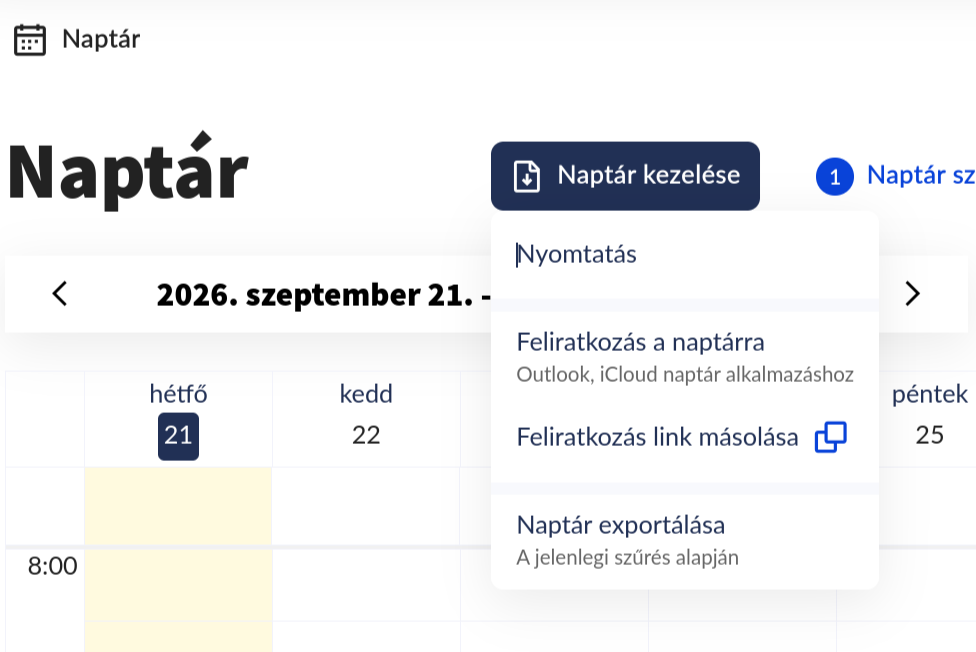
\includegraphics[width=\linewidth]{figures/neptun-calendar-export}
    \caption{Neptun: copy the subscription link.}\label{fig:neptun-export}
  \end{subfigure}\hfill
  \begin{subfigure}[b]{0.3\linewidth}
    \centering
    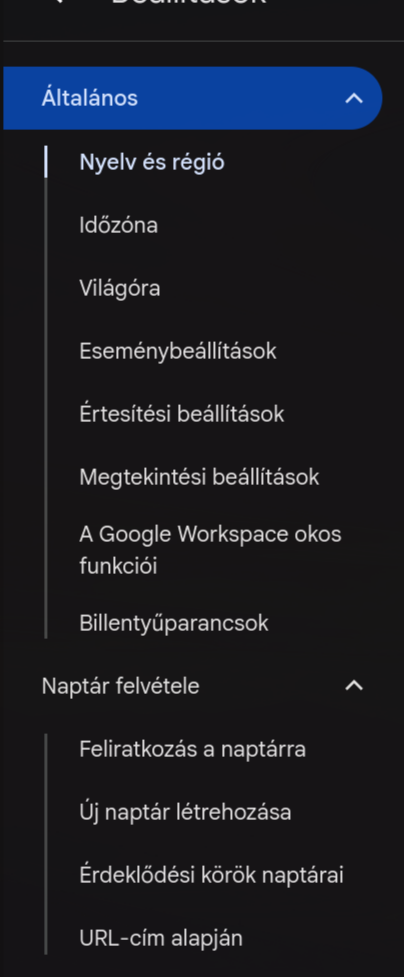
\includegraphics[width=0.75\linewidth]{figures/google-calendar-add-by-url}
    \caption{Google Calendar: add it from the URL.}\label{fig:google-calendar-url}
  \end{subfigure}
  \caption{Exporting the Neptun timetable to a calendar as a link.}\label{fig:neptun-calendar}
\end{figure}

\paragraph{Share it with your advisors.} In the Teams calendar, add your advisors' calendars: \emph{Add calendar}, type their name, add them. Ask them to give you permission to see their calendar, and share yours with them, so we can find a weekly slot (\cref{app:consult}).

\paragraph{Keeping calendars in sync.} We recommend \href{https://reclaim.ai/}{Reclaim.ai} to manage your calendar. You will likely run into permission issues with the university account; if so, \href{https://www.outlookgooglecalendarsync.com/}{Outlook Google Calendar Sync} is a workaround.

%----------------------------------------------------------------------------
\section{Development environment}\label{app:start:env}
\paragraph{Operating system.} Use Linux on bare metal if you can. We recommend \href{https://omarchy.org/}{Omarchy}, an easy-to-use distribution set up for development; ask Martin for his setup. Ubuntu and Pop!\_OS are good options too. Omarchy has a built-in Windows virtual machine; dual boot if you occasionally need Windows on bare metal. Use the Windows Subsystem for Linux (WSL) only as a last resort, if you really have to use Windows every day for a pressing reason, such as video editing.

\paragraph{Editor.} We use \href{https://code.visualstudio.com/}{Visual Studio Code}. Useful extensions: LaTeX Workshop to build the paper locally, Remote - SSH to work on the VM, GitHub Pull Requests, the Claude Code and Codex extensions, and the language extensions of your code.

\paragraph{Virtual machine.} We can give you a virtual machine with 8 cores and 16\,GB of memory in the \href{https://cloud.bme.hu/}{BME cloud}, most likely in its \href{https://fured.cloud.bme.hu/}{Füred} environment. Ask us for it directly, in the same message as your identifiers: say that you need a VM set up in the BME cloud, and we request it for you. Use it to host your editor and repositories remotely, and to run AI agents that keep working while your laptop is closed. Reach it through SSH, RDP, VS Code Remote, or Tailscale, or run Claude Code, Codex, T3 Code or GitKraken Kepler on it directly.

\paragraph{Workspace layout.} Keep one clone of the notes repository, with its \texttt{paper/} and \texttt{code/} submodules (\cref{app:code:github}), on your machine or on the VM. Open it in one VS Code window with the \LaTeX{} build and an AI agent working in the same folder, so that code, paper and notes are edited, versioned and searched together. The point is that an agent that can see the paper while it edits the code, and the consultation notes while it edits either, makes far fewer mistakes than one that sees a single repository. Commit in each submodule separately, and commit the submodule pointers in the notes repository after a consultation, so that the state you discussed is the state we can check out.

\paragraph{Do not overdo it.} Do not spend too much time on your environment setup. We learned this the hard way.

%----------------------------------------------------------------------------
\chapter{TDK essentials}\label{app:tdk}
%----------------------------------------------------------------------------
If you are working on a hard topic, show your hard work in a TDK paper: the Students' Scientific Conference (Tudományos Diákköri Konferencia) is where a semester of research turns into a reviewed, presented result.

\section{Where to look}
\begin{itemize}
  \item The \href{https://tdk.bme.hu/}{BME TDK portal} and the \href{https://tdk.bme.hu/conference/VIK/2026}{faculty's page for the current year}: check the call, the templates, the FAQ, and the review sheet. Calls change from year to year.
  \item The research group's own guide: \href{https://github.com/ftsrg/cheat-sheets/wiki/TDK-Howto}{TDK Howto} in the FTSRG cheat-sheets wiki.
  \item Past first-place papers of the research group and the department, for structure and tone.
\end{itemize}
\advisortodo{Link past first-place TDK papers of the research group and the department.}

\section{Usual deadlines}
\begin{itemize}
  \item 30 September: abstract submission on the TDK portal.
  \item 1 November: paper submission.
  \item Around 18 November: the conference.
\end{itemize}
Check the exact dates in the current call; \cref{app:lifecycle} plans the semester backwards from them.

\section{Form requirements}\label{app:tdk:form}
From the faculty call; the template already meets them.
\begin{itemize}
  \item \textbf{Length}: 30--35 pages of main text. The title page, the optional task description, the table of contents, the bibliography, the abstract and the appendices do not count.
  \item \textbf{Layout}, whether you use \LaTeX{} or Word: A4 paper, single column, Times New Roman or another readable serif font, 12\,pt, single line spacing, margins between 1.5 and 3.5\,cm on every side.
  \item \textbf{Figures and tables} are part of the main text, so they count towards the page limit. Their size is free, but they must be readable in print: avoid text below 10\,pt, labels included.
  \item The faculty's templates under \emph{Letöltések} are diploma thesis templates, so they need small changes for the TDK, such as margins and headings. This template has them.
\end{itemize}

\section{The review sheet}
Reviewers score the paper on the review sheet (bírálói lap), saved in \texttt{docs/} of this project: form and style (A, 0--5), figures and literature (B, 0--4), topic (C, 0--8), originality and soundness (D, 0--10), and introduction and evaluation (E, 0--8). The todo at the start of \tplref{chap:intro} explains the criteria and the four things to argue: relevance, non-triviality, novelty and correctness. Each chapter's todo says which of them that chapter carries.

%----------------------------------------------------------------------------
\chapter{Weekly consultations}\label{app:consult}
%----------------------------------------------------------------------------
\paragraph{Find a recurring slot.} Agree on a weekly slot with us and create a recurring MS Teams event.

\paragraph{Why every week.} A week is short enough that a wrong turn costs days, not a month, and long enough to have something to show. Come even when little has moved: a blocked week is exactly the one we can help with, and the one students tend to skip.

\paragraph{Why one-on-one.} A group meeting averages over everyone's problem, and yours is specific: your code, your draft, your plot. Alone with you we read the actual artifact and ask back until the misunderstanding is found, which takes minutes one-on-one and rarely happens in a group. It also lets us be frank about scope and effort, which is not a conversation for an audience.

\paragraph{Why in person.} In a room we share a whiteboard, which is where notation, architecture and the leading figure actually get drawn. We also see where you hesitate, which a call hides, and the hard conversations, when a topic has to be cut or re-aimed, go better face to face.

\paragraph{Consultation slides are optional.} A few slides on what you did this week, or slides that make your work easier for us to understand, save the first ten minutes of every consultation; we welcome them, LLM-generated included. A useful outline:
\begin{enumerate}[noitemsep]
  \item what you did since the last consultation, with evidence: a figure, a result, a page of text;
  \item what you read: the papers you added to Zotero this week, one sentence each on why they matter;
  \item what is blocked or where you are unsure;
  \item what you plan for next week;
  \item the questions you need us to decide.
\end{enumerate}

\paragraph{Close with a summary.} End by saying back in your own words what we agreed: the decisions, your next steps and what we owe you. Then save the same as a short written summary in your notes repository, as \texttt{notes/consultations/YYYY-MM-DD*.md}. If your summary differs from what we meant, we catch it now rather than a week of work later. The summaries are also where anchor approvals and your decisions on reviewer objections are recorded, so they are the paper's memory as much as ours.

\paragraph{The mirror principle.} We put in what you put in, and we are open about it. A student who works hard on their topic gets a lot of our time, our contacts and our help beyond the paper; a student who has put the topic on the back burner gets less of it. This is not about struggling: a student who struggles and keeps showing up gets more help, not less. It means we are mindful of where our time goes, and that you decide how much of it you get. On a separate matter, we value consistency over bursts. A student who is diligent every week and not very productive gets further than one who disappears for a month and then does brilliant work for a weekend, because research compounds: each week's result is what the next week builds on, and a weekly rhythm keeps the topic alive in your head and in ours.

\paragraph{Recordings and Teams calls.} Hold the consultation as a Teams call even when we sit in one room, and record it with transcription. You can then rewatch the details, feed the transcript to your AI tools and turn it into the notes in your repository. We recommend \href{https://github.com/openai/whisper}{Whisper} large-v3-turbo over Teams' built-in transcription: it is more accurate and handles multilingual speech better, and we usually speak a mix of Hungarian and English. Ask us for our transcription skill.

%----------------------------------------------------------------------------
\chapter{The TDK lifecycle}\label{app:lifecycle}
%----------------------------------------------------------------------------
A TDK paper comes together in the phases of \cref{tab:lifecycle}, planned backwards from the official dates of \cref{app:tdk}. Each step has an owner, a condition that says when it is done, and a pointer to what helps.
We track every student's progress in the same steps, and the weekly consultation (\cref{app:consult}) is where each step is looked at.

Three steps are \anchor{}s: the topic manifest, the spine and the full draft. An anchor is a one-page artefact that we agree on together and that everything after it is measured against. It is where your topic narrows: before the manifest, the topic is a direction; after the spine, it is a fixed set of claims with fixed names; after the full draft, it is a paper that only gets polished. Nothing stops at an anchor, but work that contradicts one is drift, and drift is the most expensive mistake in the process, because everything built on the old anchor has to be redone.

Rows marked \official{} are the official steps of the faculty's TDK: the portal dates of \cref{app:tdk:dates} are fixed, and missing one ends the semester's TDK.

\newcommand{\lcphase}[2]{\midrule\multicolumn{4}{l}{\textbf{#1}\quad\textit{#2}}\\\midrule}
{\small
\begin{xltabular}{\linewidth}{>{\raggedright\arraybackslash}p{0.2\linewidth} >{\raggedright\arraybackslash}p{0.09\linewidth} >{\raggedright\arraybackslash}X >{\raggedright\arraybackslash}p{0.21\linewidth}}
  \caption{The TDK lifecycle. Owner: you, we (the advisors), or both.}\label{tab:lifecycle}\\
  \toprule
  \textbf{Step} & \textbf{Owner} & \textbf{Done when} & \textbf{Support} \\
  \endfirsthead
  \toprule
  \textbf{Step} & \textbf{Owner} & \textbf{Done when} & \textbf{Support} \\
  \endhead
  \bottomrule
  \endlastfoot
  \lcphase{0. Topic}{before the semester}
  Topic manifest \anchor & both & One page: the problem, why it matters, the expected contribution; agreed with us & TDK topic page \\
  \lcphase{1. Setup}{first week}
  Identifiers & you & We have your Neptun code, GitHub username and e-mail & \cref{app:start:ids} \\
  Overleaf project and paper repository & we & You can edit in Overleaf and push to the synced GitHub repository & \cref{app:start:access} \\
  Repositories & you & The notes repository with \texttt{paper/} and \texttt{code/} as submodules, the code repository from the template, both advisors added to all three & \cref{app:start:access} \\
  Zotero & both & You are in the group, the connector is installed, and \texttt{bib/zotero.bib} is linked to the group through Overleaf's Zotero integration & \cref{app:start:access} \\
  Calendar and weekly slot & you & Neptun timetable synced, calendars shared, recurring Teams event set & \cref{app:start:calendar,app:consult} \\
  Virtual machine & both & You asked us for a VM, and you can reach it over SSH & \cref{app:start:env} \\
  Context upload & we & Our papers, notes and earlier work on the topic are in \texttt{notes/} of your notes repository; we commit them once you add us & --- \\
  \lcphase{2. Research}{first half of September}
  Problem & you & The problem stated with a running example & \tplref{chap:intro} \\
  Literature review (SLR) and gap analysis & you & Sources found systematically are in Zotero; the gap matrix is filled; the gap is one sentence & Gap matrix in \tplref{chap:related}; \cref{app:writing} \\
  Research questions and contributions & you & RQ1--RQ3 and C1--C3 written as checkable claims & \texttt{rqlist}, \texttt{contributions} \\
  Threats and requirements & you & Threat model, assumptions, requirements listed & \tplref{chap:intro} and \tplref{chap:approach} \\
  Leading figure draft (vezérábra) & you & \Tplref{fig:overview} explains the work without the text & \cref{app:writing:figure} \\
  Proof-of-concept implementation & you & The core idea runs end to end on the running example; shortcuts and hard-coded parts are fine & \texttt{code/} \\
  \lcphase{3. Plan}{second half of September}
  Running example and validation plan & you & The running example is named (\texttt{\textbackslash exname}) and appears in every chapter's beats; how each claim will be verified or measured is written down & \cref{app:writing:spine} \\
  Spine \anchor & both & One page of claims, terminology and notation; agreed with us & \cref{app:writing:spine} \\
  Skeleton mind map & you & Every chapter broken into paragraph topic sentences with their evidence & \cref{app:writing:spine}, \cref{fig:mindmap} \\
  Premortem & both & The paper imagined as rejected: the reviewers' likely reasons are written down, and the plan is changed to answer them & \cref{app:writing:spine} \\
  \rowcolor{official}
  Registration with the summary \official & you & Registered on the TDK portal with the one-page Hungarian and English summary, between 1 and 30 September & \cref{app:tdk:dates}; \cref{app:writing:abstract} \\
  Complete, testable implementation & you & By 30 September: every component of the approach exists, the evaluation workloads run on it, and a test suite runs, even if not every test passes yet & \tplref{chap:implementation} \\
  \lcphase{4. Draft}{October}
  Outline check & we & The skeleton fits the template's chapters and the review sheet & Chapter todos \\
  Proofs (a grind) & you & Every claim of the approach has its proof, mechanised proof, or measurement & \tplref{chap:approach} \\
  Tested implementation (a grind) & you & All tests pass, and \texttt{just reproduce} regenerates every result from the README; the release is ready for Zenodo & \cref{app:code:github} \\
  Scalability and robustness & you & Measurements beyond small examples, with setup and repetitions, and a robustness analysis that perturbs the system on purpose & \tplref{fig:scalability} and \tplref{tab:robustness} \\
  Full draft \anchor & both & Every chapter written; handed to us about ten days before the deadline & --- \\
  \lcphase{5. Polish}{the last ten days of October; see \cref{tab:polish}}
  Advisor review and todos & both & Our comments are resolved; the list of todos is empty & \texttt{\textbackslash listoftodos} \\
  Review sheet hill climb & you & You scored the paper on criteria A--E yourself, fixed the weakest, and repeated until nothing cheap is left & Review sheet in \texttt{docs/}; \cref{app:tdk:sheet} \\
  Last week's checklist & you & Every row of \cref{tab:polish} is checked; \texttt{make check} is clean & \cref{tab:polish} \\
  Code archive & you & The code is on Zenodo and cited by its concept DOI; the tag the results came from is named in the paper & \cref{app:zenodo} \\
  \rowcolor{official}
  Paper upload \official & you & The AI declaration, after the bibliography, is filled in, the main text is 30--35 pages, and the PDF is uploaded on the portal by 1 November & \cref{app:tdk:form} \\
  \lcphase{6. After the deadline}{2--16 November, while the reviewers read}
  Code polish & you & The README meets \cref{app:code:readme}, the Docker images build (\cref{app:code:docker}), and a new Zenodo version is published; the results tag named in the paper is untouched & \cref{app:zenodo:versions} \\
  Talk & you & Slides ready and rehearsed with us at least once before the conference & --- \\
  \lcphase{7. Conference}{18 November}
  \rowcolor{official}
  Conference \official & you & Fifteen minutes of talk and five of questions in your section; the awards are the same evening & \cref{app:tdk:dates} \\
  After the TDK & both & Decided together: OTDK, a conference paper, or a thesis built on the work & --- \\
\end{xltabular}
}

\section{Last week's checklist}\label{app:lifecycle:polish}
The polish phase is a checklist, not a phase of writing: if a row needs more than an hour, it belongs to the draft phase and the draft was not full. \texttt{make check} runs the mechanical rows on the build log; the rest you check by reading.
{\small
\begin{xltabular}{\linewidth}{>{\raggedright\arraybackslash}p{0.26\linewidth} X}
  \caption{Last week's checklist. The mechanical rows are also checked by \texttt{make check}.}\label{tab:polish}\\
  \toprule \textbf{Check} & \textbf{Done when} \\ \midrule \endfirsthead
  \toprule \textbf{Check} & \textbf{Done when} \\ \midrule \endhead
  \bottomrule \endlastfoot
  Page count & The main text, from the first page of \tplref{chap:intro} to the last page of \tplref{chap:conclusion}, is 30--35 pages; appendices, the bibliography, the abstract and the title page do not count. \texttt{make check} prints it. \\
  Build log & No undefined or multiply defined labels, no undefined citations, no overfull boxes, no missing fonts or files. \\
  Cross-references & Every reference uses \texttt{\textbackslash cref}; every figure, table, listing and equation is referenced from the text (\cref{app:latex:cref}). \\
  Figures are vector & Every figure is TikZ in the paper repository, or has a written reason not to be; a draw.io draft was redrawn or exported as PDF only as a last resort (\cref{app:writing:figure}). \\
  Axes and legends & Every axis has a label with a unit; every legend entry names a thing the text also names. \\
  Captions & Every caption explains the figure in the sense of \cref{app:writing:captions}: a claim first, then context. \\
  Readable in print & No text in a figure is below 10\,pt when printed; colour pairs are distinguishable in greyscale. \\
  Tables & Tables fit the text width, numbers are right-aligned with the same precision in a column, units are in the header. \\
  Spine drift & Every term, symbol and claim matches the spine; one name per concept across chapters. \\
  Citations & Every claim from the literature is cited; bibliography entries have author, title, venue and year; DOIs where they exist; capitalisation protected with braces (\cref{app:latex:cite}). \\
  Acronyms & Every abbreviation goes through \texttt{\textbackslash ac}, and the list of acronyms contains only those used (\cref{app:latex:acro}). \\
  Front and back matter & Title page variables, abstract in both languages, the AI declaration, acknowledgements and the appendices are filled in; no \enquote{TODO} remains in the PDF. \\
  Notes removed & \texttt{final} is set in the document class options, \texttt{\textbackslash listoftodos} is removed, and no beat, todo or advisor note prints (\cref{app:latex:todo}). \\
  Guide removed & The guide is deleted from \texttt{thesis.tex}. \\
  PDF & Bookmarks and metadata are correct, every link resolves, and the Zenodo DOI opens the record. \\
  Spelling and language & A spell check in the paper's language passed; British or American spelling is consistent. \\
  Reproducibility & \texttt{docker run \dots{} reproduce} regenerates every figure and table from the results tag named in the paper (\cref{app:code:readme}). \\
  Review sheet & You scored the paper on criteria A--E yourself, and nothing cheap is left to fix (\cref{app:tdk:sheet}). \\
\end{xltabular}
}

%----------------------------------------------------------------------------
\chapter{Writing}\label{app:writing}
%----------------------------------------------------------------------------
\section{Plan before you write: problem to skeleton}\label{app:writing:spine}
Write the argument before the prose. We plan papers in this order, and each step builds on the previous one: problem; context and literature review; gap analysis; research questions; contributions; threat analysis; leading figure; examples; validation plan; spine; figures; skeleton; beats.
\begin{description}
  \item[Problem] The entry point, and the only step you need to start. One paragraph: who has what problem, what goes wrong for them today, and one concrete scenario in which it goes wrong. The scenario becomes the running example, and the paragraph becomes the first page of \tplref{ch:intro}. If you can write it, you can start the literature review; if you cannot, bring what you have to the next consultation and we write it together.
  \item[Spine] One page that fixes the claims, the terminology and the notation of the whole paper. Every chapter, figure and review is checked against it. Its worst enemy is drift: terms, symbols and claims quietly changing between chapters.
  \item[Skeleton mind map] The argument made explicit before any prose: each chapter broken into paragraphs, each paragraph reduced to its topic sentence and a pointer to the evidence that backs it. Drafting then means filling in sentences around a skeleton already known to be sound. A mind map, on paper or in a tool, is the quickest way to draw it; \cref{fig:mindmap} shows one for the guide's running example, a made-up paper, at the level of detail we expect. \Cref{fig:template-skeleton} is the same picture for this template's own beats: the generic argument every chapter file starts from. Your skeleton is built per topic and will not look like either; what carries over is the shape.
  \item[Running example] One concrete scenario that every chapter returns to. Name it once with \texttt{\textbackslash exname} in \texttt{thesis.tex}, introduce it in \tplref{ch:intro}, and revisit it in every chapter in a \texttt{runningexample} box: what each concept, component, measurement or competitor does with it. A reader who follows only the boxes should understand the paper.
  \item[Beats] The moves inside each paragraph of the skeleton: what it establishes, which evidence it uses, what the running example shows there, and how it leads to the next one. \Cref{app:chapters} gives every heading of the template the generic beat of its paragraph. Write your own, specific to your topic, at the top of each paragraph you plan: \texttt{\textbackslash beat\{establishes\}\{evidence\}\{running example\}\{leads to\}}. It prints as a todo, so it disappears from the final version.
\end{description}

\begin{figure}[p]
  \centering
  \begin{forest}
    for tree={
      grow'=0, child anchor=west, parent anchor=east, anchor=west,
      font=\scriptsize, edge={gray!60},
      l sep=6mm, s sep=1.2pt, inner sep=1.5pt,
      edge path={\noexpand\path[\forestoption{edge}](!u.parent anchor) -- +(3mm,0) |- (.child anchor)\forestoption{edge label};},
    },
    where level=0{text width=2.4cm, font=\footnotesize}{},
    where level=1{text width=2.5cm}{},
    where level=2{text width=9.3cm}{},
    [{\textbf{Revoking\\credentials\\with bounded\\staleness}}
      [{\textbf{1 Introduction}}
        [{Digital credentials are checked offline, so a revocation must reach the verifier another way \textit{[incident report, cited]}}]
        [{Running example: a revoked diploma that an employer still accepts, because its status copy is stale}]
        [{REQ1 timely revocation (within $\delta$), REQ2 offline checks, REQ3 holder privacy \textit{[Tab. 6.1]}}]
        [{Gap: no existing approach meets REQ1--REQ3 together \textit{[approaches, cited]}}]
        [{C1 model, C2 registry, C3 evaluation; RQ1 correctness, RQ2 scalability, RQ3 robustness \textit{[Fig. 1.1]}}]
      ]
      [{\textbf{2 Background}}
        [{Issuer, holder, verifier; what a revocation status is and how stale a copy can be \textit{[definition, cited]}}]
        [{Accumulators: membership witness, update cost \textit{[definition, cited]}}]
        [{Permissioned ledgers: writers, readers, finality \textit{[definition, cited]}}]
        [{Dolev--Yao adversary and the Tamarin prover \textit{[tool paper, cited]}}]
      ]
      [{\textbf{3 Approach}}
        [{Overview: a check reads one accumulator witness \textit{[Fig. 3.1]}}]
        [{Model: registry state, revocation, staleness of a verifier's copy \textit{[Def. 3.1]}}]
        [{Check: one witness, offline (REQ2), credential not named (REQ3) \textit{[Alg. 3.1]}}]
        [{Adversary: ADV1 a malicious holder replaying an old status proof, ADV2 a Dolev--Yao network adversary \textit{[ADV1--ADV2]}}]
        [{Assumptions: AS1 sound signatures and accumulator, AS2 clock drift at most $\delta$, AS3 honest-but-curious operator \textit{[AS1--AS3]}}]
        [{Out of scope: denial of service, compromised holder devices}]
        [{Lemma 3.1: status proofs are fresh \textit{[Tamarin model; AS1, AS2]}}]
        [{Theorem 3.1 = SG1: under AS1--AS3, against ADV1 and ADV2, a verifier rejects every credential revoked more than $\delta$ before the check \textit{[Tamarin proof]}}]
        [{Example: the diploma presented with an old status proof is rejected}]
      ]
      [{\textbf{4 Implementation}}
        [{Architecture: registry service, verifier library, reused ledger \textit{[Fig. 3.1]}}]
        [{Design: signed accumulator values, not ledger reads \textit{[alternative rejected]}}]
        [{The verifier's check: signed and younger than $\delta$ \textit{[listing, tests]}}]
        [{Code and scripts archived on Zenodo, with the rerun command \textit{[archived code]}}]
      ]
      [{\textbf{5 Evaluation}}
        [{Setup: one 8-core cloud VM, 10 runs, fresh issuer sets \textit{[rerun command]}}]
        [{RQ1 correctness: proofs per guarantee, tests per requirement \textit{[Tab. 5.1]}}]
        [{The scenario before and after, as a sequence chart \textit{[Fig. 5.1]}}]
        [{RQ2 scalability: checks stay within one round trip up to 10\,000 issuers; a list-based baseline grows linearly \textit{[Fig. 5.2]}}]
        [{Storage grows with the credentials ever issued \textit{[Fig. 5.2]}}]
        [{RQ3 robustness: a ledger node crash, a revocation burst, clock drift and $\delta$ varied \textit{[Tab. 5.2, Fig. 5.3]}}]
        [{Threats to validity: synthetic issuer sets, one cloud VM}]
      ]
      [{\textbf{6 Related work}}
        [{Family A: how it works, which of REQ1--REQ3 it gives up \textit{[approaches, cited]}}]
        [{Family B: how it works, which of REQ1--REQ3 it gives up \textit{[approaches, cited]}}]
        [{Family C: how it works, which of REQ1--REQ3 it gives up \textit{[approaches, cited]}}]
        [{Gap matrix: no family meets REQ1--REQ3 together \textit{[Tab. 6.1, Fig. 6.1]}}]
      ]
      [{\textbf{7 Conclusion}}
        [{C1--C3 restated with their evidence \textit{[Thm 3.1, Fig. 5.2, Tab. 5.1]}}]
        [{LIM1 synthetic workloads \textit{[threats to validity]}}]
        [{LIM2 the registry cannot force an issuer to revoke \textit{[scope of SG1]}}]
        [{Future work: real issuer workloads; holding issuers to their revocation duty}]
      ]
    ]
  \end{forest}
  \caption{A skeleton mind map for the guide's running example, the credential revocation registry, whose items \cref{app:chapters} renders chapter by chapter, so one paper can be followed from skeleton to items. Every leaf is one paragraph's topic sentence, and the bracketed italics name the evidence behind it: a theorem, a model, a table, a figure or a citation. A skeleton at this level of detail shows whether the argument holds before a sentence of prose exists, and it is what the spine anchor of \cref{tab:lifecycle} is checked against. Copy the shape, not the topic: one leaf per paragraph, evidence on every leaf that makes a claim, and the running example visible in every chapter.}\label{fig:mindmap}
\end{figure}


\begin{figure}[p]
  \centering
  \begin{forest}
    for tree={
      grow'=0, child anchor=west, parent anchor=east, anchor=west,
      font=\scriptsize, edge={gray!60},
      l sep=6mm, s sep=1.2pt, inner sep=1.5pt,
      edge path={\noexpand\path[\forestoption{edge}](!u.parent anchor) -- +(3mm,0) |- (.child anchor)\forestoption{edge label};},
    },
    where level=0{text width=2.4cm, font=\footnotesize}{},
    where level=1{text width=2.5cm}{},
    where level=2{text width=9.3cm}{},
    [{\textbf{The template's beats}}
      [{\textbf{1 Introduction}}
        [{Context: why the field matters now \textit{[a trend, a regulation or an incident, cited]}}]
        [{Problem: the concrete problem, ending in a one-sentence statement \textit{[the running example]}}]
        [{Requirements: what a solution must do \textit{[one requirement per failure of the example; the rows of the gap matrix]}}]
        [{Gap: no existing approach meets them together \textit{[the closest approaches, cited]}}]
        [{Contributions: what this work claims, as checkable items \textit{[the chapters behind each]}}]
      ]
      [{\textbf{2 Background}}
        [{The first concept the approach relies on; notation defined once \textit{[a definition and a citation]}}]
        [{The second concept \textit{[a definition and a citation]}}]
      ]
      [{\textbf{3 Approach}}
        [{Overview: how it works end to end \textit{[the architecture figure]}}]
        [{The formal model or the design decisions \textit{[each decision with the alternative rejected]}}]
        [{Threat model: the adversary's capabilities, who is trusted, the cryptographic assumptions, what is out of scope, and the guarantees \textit{[a proof, a mechanised proof or a measurement per guarantee]}}]
      ]
      [{\textbf{4 Implementation}}
        [{What was built and how it realises the approach \textit{[components mapped to code; the archived artifact]}}]
        [{Design decisions and the problems a straightforward build runs into \textit{[each with the alternative rejected]}}]
        [{The part that did not exist before \textit{[the key listing and the tests that cover it]}}]
      ]
      [{\textbf{5 Evaluation}}
        [{Setup: how the measurements were made \textit{[hardware, versions, workloads, repetitions, the rerun command]}}]
        [{Correctness on the example and on every requirement case \textit{[test, proof or model-checking results]}}]
        [{How the cost grows with the input \textit{[the scalability figure]}}]
        [{Behaviour when the assumptions are stressed \textit{[the robustness table, with each perturbation's setup]}}]
        [{Threats to validity and what was done about each \textit{[the mitigations]}}]
      ]
      [{\textbf{6 Related work}}
        [{How each family of approaches works and where it falls short \textit{[citations, the positioning figure and the gap matrix]}}]
        [{The gap in one sentence, closed by this work \textit{[the gap matrix and the evaluation results]}}]
      ]
      [{\textbf{7 Conclusion}}
        [{Each contribution and its evidence \textit{[the chapters behind C1--C3]}}]
        [{What is still open, and the next step for each limitation \textit{[the threats to validity]}}]
      ]
    ]
  \end{forest}
  \caption{The template's own beats drawn as a skeleton: one leaf per beat of \cref{app:chapters}, the topic it establishes first and its evidence in brackets. This is the generic argument the template starts you from, not a skeleton to copy: \cref{fig:mindmap} shows what a topic's own skeleton looks like once the claims, examples and evidence are specific, and yours will have more leaves where your contribution is and fewer elsewhere.}\label{fig:template-skeleton}
\end{figure}

\section{The essentials}\label{app:writing:essentials}
Every paper of this kind contains the same two dozen elements, whatever its topic: a problem statement, requirements, a leading figure, a threat model, research questions, a gap matrix, a summary with its evidence, and the rest of the list below. They are the leaves of \cref{fig:template-skeleton} that a reviewer looks for by name, and the review sheet scores each of them somewhere; the letter after each row names the criterion. The lint calls them the \emph{essentials} and measures every paper against the same list, so the Checks page at the front of the draft shows where yours stands, and the job summary of your repository's CI opens with the same marks in one line. The list lives in \texttt{scripts/lint/essentials.lua}, and this section is printed from it by \texttt{make essentials}: delete the template's skeleton chapters and the list still holds. Each row links to the same item in action in \cref{app:chapters}.

% generated by texlua scripts/lint.lua essentials --guide (make essentials); do not edit
\definecolor{lintaccent}{RGB}{155,28,28}\definecolor{lintmute}{gray}{0.38}
\providecommand{\lintdisc}[3]{\tikz[baseline=-.6ex]{\draw[#2,line width=.45pt,fill=white] (0,0) circle (#1);\ifcase#3\relax\or\fill[#2] (0,0) -- (0,#1) arc[start angle=90,end angle=0,radius=#1] -- cycle;\or\fill[#2] (0,0) -- (0,#1) arc[start angle=90,end angle=-90,radius=#1] -- cycle;\or\fill[#2] (0,0) -- (0,#1) arc[start angle=90,end angle=-180,radius=#1] -- cycle;\or\fill[#2] (0,0) circle (#1);\fi}}
\providecommand{\lintball}[2][black]{\lintdisc{.62ex}{#1}{#2}}
\providecommand{\lintbigball}[2][black]{\lintdisc{.8ex}{#1}{#2}}
The lint places each essential on a ladder of five levels: \lintball{0} missing; \lintball{1} a placeholder, only TODO or the template's own text; \lintball{2} started, your own text but not enough of it; \lintball{3} written; \lintball{4} used where the argument needs it. An essential with no condition for its use is \lintball{4} once written. The phase in \texttt{thesis.tex} asks every essential for a level: \textsc{plan} \lintball{1}, \textsc{draft} \lintball{2}, \textsc{polish} and \textsc{final} \lintball{4}. An essential is found by its label first, then by a heading that contains one of the words given. Text is your own when it is neither a TODO line nor a line of the template, and floats, tagged lists and example boxes count toward their own essentials, not toward the text around them.

{\small\begin{xltabular}{\linewidth}{@{}>{\raggedright\arraybackslash}p{.25\linewidth}>{\raggedright\arraybackslash}X>{\raggedright\arraybackslash}p{.3\linewidth}@{}}
\toprule \textbf{Essential} & \textbf{What it is, and why} & \textbf{Written, and used} \\ \midrule \endfirsthead
\toprule \textbf{Essential} & \textbf{What it is, and why} & \textbf{Written, and used} \\ \midrule \endhead \bottomrule \endlastfoot
\multicolumn{3}{@{}l}{\textsc{Front matter}} \\
\textbf{Abstract and Kivonat}\newline{\footnotesize\color{lintmute}\texttt{\textbackslash chapter*\{Kivonat\}} and \texttt{\{Abstract\}}}\newline{\footnotesize In action: \cref{app:writing:abstract}} & The paper in one paragraph, in English and in Hungarian; the reviewer reads it first and the registration carries it.\hfill{\footnotesize\color{lintmute}(E)} & 100 own words in each.\newline Written is enough. \\
\addlinespace[.8ex]\multicolumn{3}{@{}l}{\textsc{Introduction}} \\
\textbf{Context}\newline{\footnotesize\color{lintmute}\texttt{par:context}, or a heading with \emph{context} or \emph{motivation}}\newline{\footnotesize In action: \cref{app:chapters:context}} & Why the topic matters now: a trend, a regulation or an incident, cited; relevance is scored in C.\hfill{\footnotesize\color{lintmute}(C, E)} & 40 own words.\newline Written is enough. \\
\textbf{Problem statement}\newline{\footnotesize\color{lintmute}\texttt{par:problem}, or a heading with \emph{problem}}\newline{\footnotesize In action: \cref{app:chapters:problem}} & The concrete problem, ending in a one-sentence statement; the sheet's E names the problem statement as a must.\hfill{\footnotesize\color{lintmute}(E)} & 40 own words.\newline Written is enough. \\
\textbf{Running example}\newline{\footnotesize\color{lintmute}\texttt{\textbackslash exname} and the example box}\newline{\footnotesize In action: \cref{app:chapters:problem}} & One small scenario, named once in thesis.tex (\textbackslash{}exname) and revisited in a box in every chapter, so the reader can follow each step.\hfill{\footnotesize\color{lintmute}(A)} & Named, and the introduction's box in your own words.\newline Used when an example box in every main chapter. \\
\textbf{Requirements}\newline{\footnotesize\color{lintmute}items labelled \texttt{req:}}\newline{\footnotesize In action: \cref{app:chapters:requirements}} & What a solution must do, one checkable item each; they are the rows of the gap matrix and the yardstick of the evaluation.\hfill{\footnotesize\color{lintmute}(D/1)} & Every item in your own words.\newline Used when each requirement is referenced in the related work and in the evaluation, and each derived requirement (dr:) in the evaluation. \\
\textbf{Gap, in brief}\newline{\footnotesize\color{lintmute}\texttt{par:gap}, or a heading with \emph{gap}}\newline{\footnotesize In action: \cref{app:chapters:introgap}} & That no existing approach meets the requirements together; the novelty claim, made before the full comparison.\hfill{\footnotesize\color{lintmute}(D/1)} & 40 own words.\newline Used when it points to the full comparison: the related-work chapter, the gap matrix or the positioning figure. \\
\textbf{Leading figure}\newline{\footnotesize\color{lintmute}\texttt{fig:overview}}\newline{\footnotesize In action: \cref{fig:guide:overview}} & The problem, the contributions and the headline result in one picture; the reviewer looks here first.\hfill{\footnotesize\color{lintmute}(B/1)} & Your own content, and a caption of at least a sentence.\newline Used when it is referenced from the text. \\
\textbf{Contributions}\newline{\footnotesize\color{lintmute}items labelled \texttt{c:}}\newline{\footnotesize In action: \cref{app:chapters:contributions}} & What this work claims, as checkable items; the sheet's E names stating the main contribution as a must.\hfill{\footnotesize\color{lintmute}(E)} & Every item in your own words.\newline Used when each contribution points to the chapter that delivers it and is referenced in the conclusion. \\
\addlinespace[.8ex]\multicolumn{3}{@{}l}{\textsc{Approach}} \\
\textbf{Architecture figure}\newline{\footnotesize\color{lintmute}\texttt{fig:architecture}}\newline{\footnotesize In action: \cref{fig:guide:architecture}} & The approach end to end, with what is yours set apart from what is reused.\hfill{\footnotesize\color{lintmute}(B/1)} & Your own content, and a caption of at least a sentence.\newline Used when it is referenced from the text. \\
\textbf{Threats}\newline{\footnotesize\color{lintmute}items labelled \texttt{thr:}}\newline{\footnotesize In action: \cref{app:chapters:adversary}} & Who the adversary is and what it can do; a reviewer of a security topic looks for it first.\hfill{\footnotesize\color{lintmute}(D/2)} & Every item in your own words.\newline Used when each threat is referenced in the approach, where a guarantee or an assumption meets it. \\
\textbf{Assumptions}\newline{\footnotesize\color{lintmute}items labelled \texttt{asm:}}\newline{\footnotesize In action: \cref{app:chapters:assumptions}} & Who is trusted and which properties the guarantees rest on, stated so a reviewer can check them.\hfill{\footnotesize\color{lintmute}(D/2)} & Every item in your own words.\newline Used when each assumption is referenced in the approach, by a guarantee or a proof. \\
\textbf{Guarantees}\newline{\footnotesize\color{lintmute}items labelled \texttt{g:}}\newline{\footnotesize In action: \cref{app:chapters:guarantees}} & What the approach guarantees under the assumptions, against the threats; each is what the evaluation checks.\hfill{\footnotesize\color{lintmute}(D/2)} & Every item in your own words.\newline Used when each guarantee is referenced in the evaluation, as a row of the correctness table. \\
\addlinespace[.8ex]\multicolumn{3}{@{}l}{\textsc{Evaluation}} \\
\textbf{Research questions}\newline{\footnotesize\color{lintmute}items labelled \texttt{rq:}}\newline{\footnotesize In action: \cref{app:chapters:research-questions}} & The questions the evaluation answers: correctness, scale and robustness at least.\hfill{\footnotesize\color{lintmute}(E)} & Every item in your own words.\newline Used when each research question is referenced in the evaluation, where it is answered. \\
\textbf{Setup and artifact}\newline{\footnotesize\color{lintmute}\texttt{sec:setup}, or a heading with \emph{setup}}\newline{\footnotesize In action: \cref{app:chapters:setup}} & How the measurements were made, so each can be checked, and where the archived artifact is.\hfill{\footnotesize\color{lintmute}(D/2)} & 100 own words.\newline Used when the evaluation cites the archived artifact with a real DOI. \\
\textbf{Correctness}\newline{\footnotesize\color{lintmute}\texttt{tab:correctness}}\newline{\footnotesize In action: \cref{tab:guide:correctness}} & How each guarantee and requirement was checked: proved, tested or model-checked, with the result.\hfill{\footnotesize\color{lintmute}(D/2)} & Your own content, and a caption of at least a sentence.\newline Used when it is referenced from the text, and every guarantee (g:) has a row in it. \\
\textbf{Scalability}\newline{\footnotesize\color{lintmute}\texttt{sec:scalability}, or a heading with \emph{scalab} or \emph{scaling} or \emph{performance}}\newline{\footnotesize In action: \cref{app:chapters:scalability}} & How the cost grows with the input; the review sheet scores the evaluation's depth in E.\hfill{\footnotesize\color{lintmute}(E)} & 100 own words.\newline Used when the section holds a figure or table that the text references. \\
\textbf{Robustness}\newline{\footnotesize\color{lintmute}\texttt{sec:robustness}, or a heading with \emph{robust}}\newline{\footnotesize In action: \cref{app:chapters:robustness}} & How the system behaves when its assumptions are stressed; scored apart from scalability.\hfill{\footnotesize\color{lintmute}(E)} & 100 own words.\newline Used when the section holds a figure or table that the text references. \\
\textbf{Threats to validity}\newline{\footnotesize\color{lintmute}\texttt{sec:validity}, or a heading with \emph{validity}}\newline{\footnotesize In action: \cref{app:chapters:validity}} & What could make the results wrong or not generalise, and what was done about each.\hfill{\footnotesize\color{lintmute}(D/2)} & 100 own words.\newline Written is enough. \\
\addlinespace[.8ex]\multicolumn{3}{@{}l}{\textsc{Related work}} \\
\textbf{Positioning figure}\newline{\footnotesize\color{lintmute}\texttt{fig:positioning}}\newline{\footnotesize In action: \cref{fig:guide:positioning}} & The related work on the two properties that separate it most, with this work in the cell no one else reaches.\hfill{\footnotesize\color{lintmute}(B/2)} & Your own content, and a caption of at least a sentence.\newline Used when it is referenced from the text. \\
\textbf{Gap matrix}\newline{\footnotesize\color{lintmute}\texttt{tab:related}}\newline{\footnotesize In action: \cref{tab:guide:related}} & Each requirement against the closest approaches: every other approach misses something, this work meets all.\hfill{\footnotesize\color{lintmute}(D/1)} & Your own content, and a caption of at least a sentence.\newline Used when rows are the requirements, this work's column is all met with pointers to results, and every other approach misses one. \\
\textbf{The gap}\newline{\footnotesize\color{lintmute}\texttt{sec:gap}, or a heading with \emph{gap}}\newline{\footnotesize In action: \cref{app:chapters:gap}} & The gap in one sentence, shown closed by this work's results.\hfill{\footnotesize\color{lintmute}(D/1)} & 100 own words.\newline Used when it is based on the gap matrix (references tab:related). \\
\addlinespace[.8ex]\multicolumn{3}{@{}l}{\textsc{Conclusion}} \\
\textbf{Summary with evidence}\newline{\footnotesize\color{lintmute}\texttt{sec:summary}, or a heading with \emph{summary}}\newline{\footnotesize In action: \cref{app:chapters:summary}} & Each contribution restated with the result behind it; the reviewer checks here that the promises were kept.\hfill{\footnotesize\color{lintmute}(E)} & 100 own words.\newline Used when it cites an evaluation result: the evaluation chapter, a research question, a figure, a table or a theorem. \\
\textbf{Limitations}\newline{\footnotesize\color{lintmute}items labelled \texttt{lim:}}\newline{\footnotesize In action: \cref{app:chapters:future}} & What this work does not do, stated before a reviewer finds it.\hfill{\footnotesize\color{lintmute}(E)} & Every item in your own words.\newline Written is enough. \\
\textbf{Future work}\newline{\footnotesize\color{lintmute}\texttt{sec:future}, or a heading with \emph{future}}\newline{\footnotesize In action: \cref{app:chapters:future}} & What is still open, and the next step that would lift each limitation.\hfill{\footnotesize\color{lintmute}(E)} & 100 own words.\newline Written is enough. \\
\end{xltabular}}


\section{The leading figure (vezérábra)}\label{app:writing:figure}
The leading figure (\tplref{fig:overview}) explains the central idea in one picture: the problem, the contributions, and the result. Decide what a reader should take away from it, draw that, and write the caption so that the figure stands without the text. Make what is yours visible at a glance. The template's figures use one colour for everything that is yours, blue, through the \texttt{ours} TikZ style; the problem is red, the result green, and reused or external parts are grey (\texttt{prior}). Every work has at least two components, and all of them get the same blue, so the reader sees the extent of your contribution in one look; the caption says which colour is which. A reviewer who cannot tell your contribution from the surrounding system in the first figure will assume the smaller part is yours. Draft it early, in the research phase, and treat it as exploratory until the spine is agreed: many papers find their argument while drawing it. \Cref{fig:collage} shows the leading figures of four papers from our group.

\begin{figure}[!ht]
  \centering
  \begin{subfigure}[t]{0.48\linewidth}
    \centering
    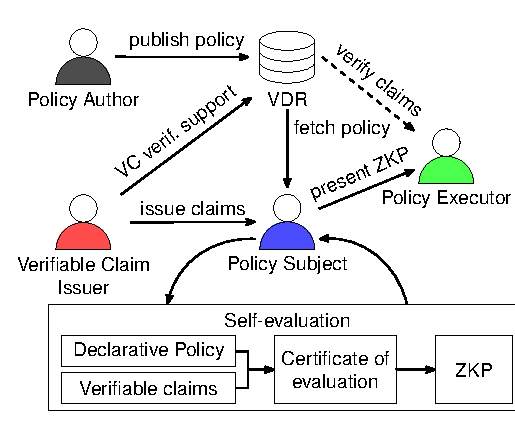
\includegraphics[width=\linewidth,height=5.2cm,keepaspectratio]{guide/figures/collage/eurocybersec2024}
    \caption{A policy is evaluated by its own subject and proven in zero knowledge: the actors and the flows between them, nothing else.}\label{fig:collage:ecs}
  \end{subfigure}\hfill
  \begin{subfigure}[t]{0.48\linewidth}
    \centering
    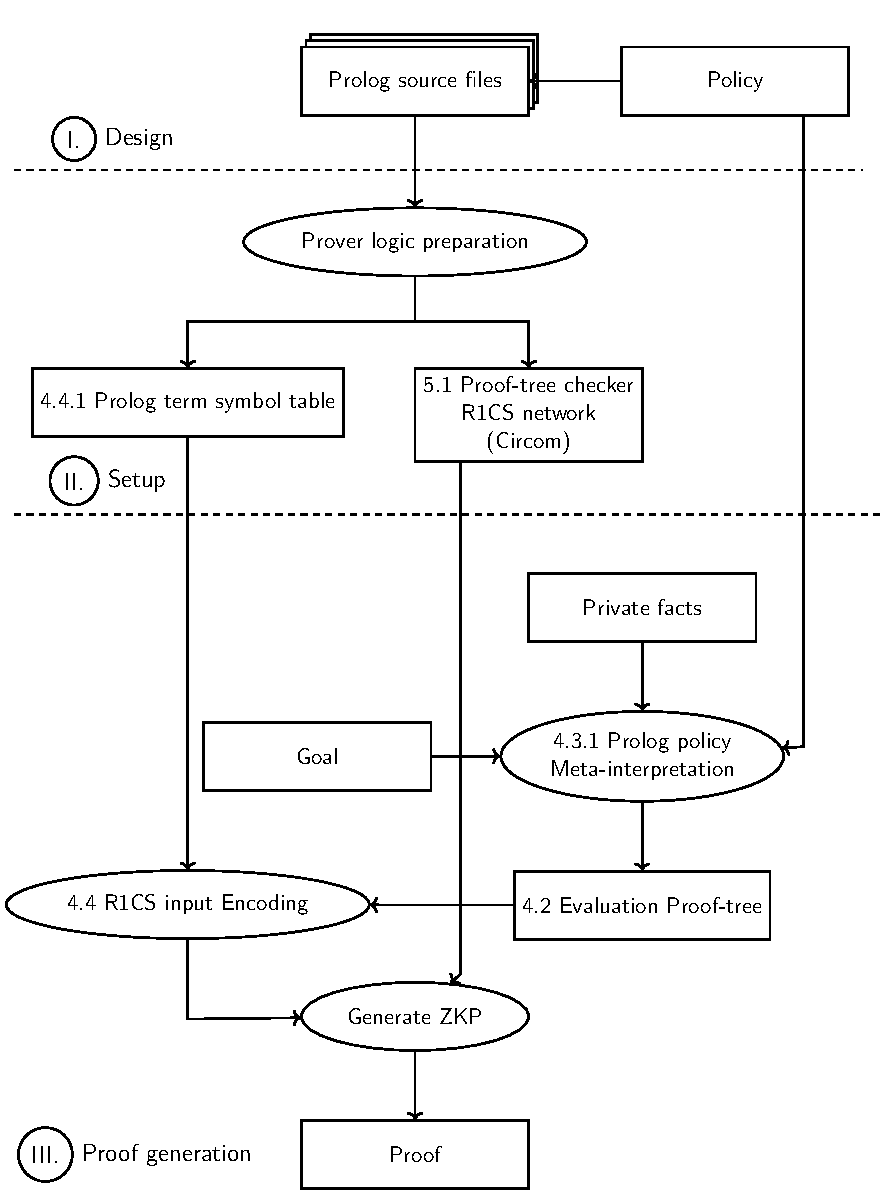
\includegraphics[width=\linewidth,height=5.2cm,keepaspectratio]{guide/figures/collage/tdk2023}
    \caption{The toolchain of the same idea as a TDK paper: every stage from policy to proof, so the reader sees where the contribution sits.}\label{fig:collage:tdk}
  \end{subfigure}

  \medskip
  \begin{subfigure}[t]{0.48\linewidth}
    \centering
    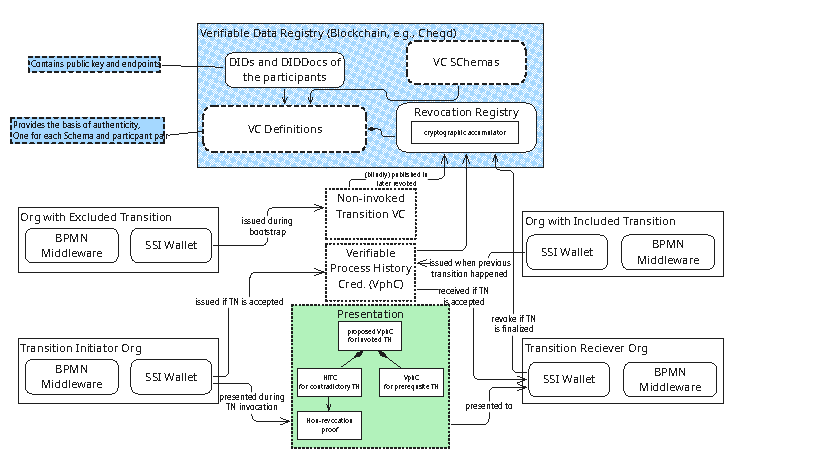
\includegraphics[width=\linewidth,height=5.2cm,keepaspectratio]{guide/figures/collage/bpm2025}
    \caption{Self-orchestrated business collaborations: the architecture with the data model folded in, one picture for both.}\label{fig:collage:bpm25}
  \end{subfigure}\hfill
  \begin{subfigure}[t]{0.48\linewidth}
    \centering
    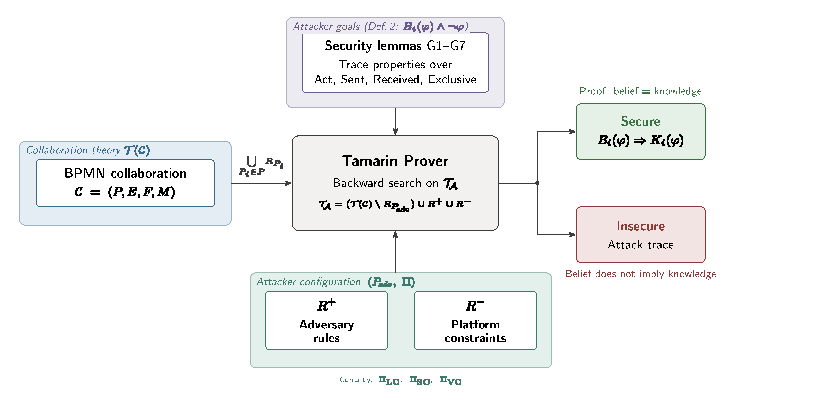
\includegraphics[width=\linewidth,height=5.2cm,keepaspectratio]{guide/figures/collage/bpm2026}
    \caption{From a BPMN collaboration to a security analysis: inputs on the left, the method in the middle, the verdicts on the right.}\label{fig:collage:bpm26}
  \end{subfigure}
  \caption{Leading figures of four papers from the group: (a) the EuroCyberSec 2024 workshop paper on self-evaluated policies~\cite{guide:farkas2024selfevaluated}, (b) the 2023 TDK paper it grew out of~\cite{guide:farkas2023tdk}, (c) the self-orchestration model for business collaborations~\cite{guide:farkas2025selforchestration}, and (d) the formal security analysis of BPMN collaborations~\cite{guide:farkas2026trustnopool}. Each one shows the problem, the contribution and the result in a single picture, and each was drawn before the paper was written.}\label{fig:collage}
\end{figure}

When the contribution is spread over several chapters, \cref{app:writing:depgraph} draws the whole paper instead.

\section{An alternative: the paper as a dependency graph}\label{app:writing:depgraph}
The skeleton mind map (\cref{fig:mindmap}) is a tree of chapters and their paragraphs. Draw an arrow from each paragraph to every paragraph that needs it, and the tree becomes a dependency graph of the paper (\cref{fig:depgraph}). Lay it out in bands, one per chapter in reading order, with each band's paragraphs in their order in the chapter. Colour green the paragraphs that deliver a contribution, tag each with its contribution, and leave the rest white. The green is for the reviewer: before reading a sentence, they see where your contribution is, how much of the paper it fills, what it stands on, and which evaluation question tests it. Green marks paragraphs here, not components, so the architecture figure keeps the blue of \texttt{ours} for the parts of the system you built.

\begin{figure}[!ht]
  \centering
  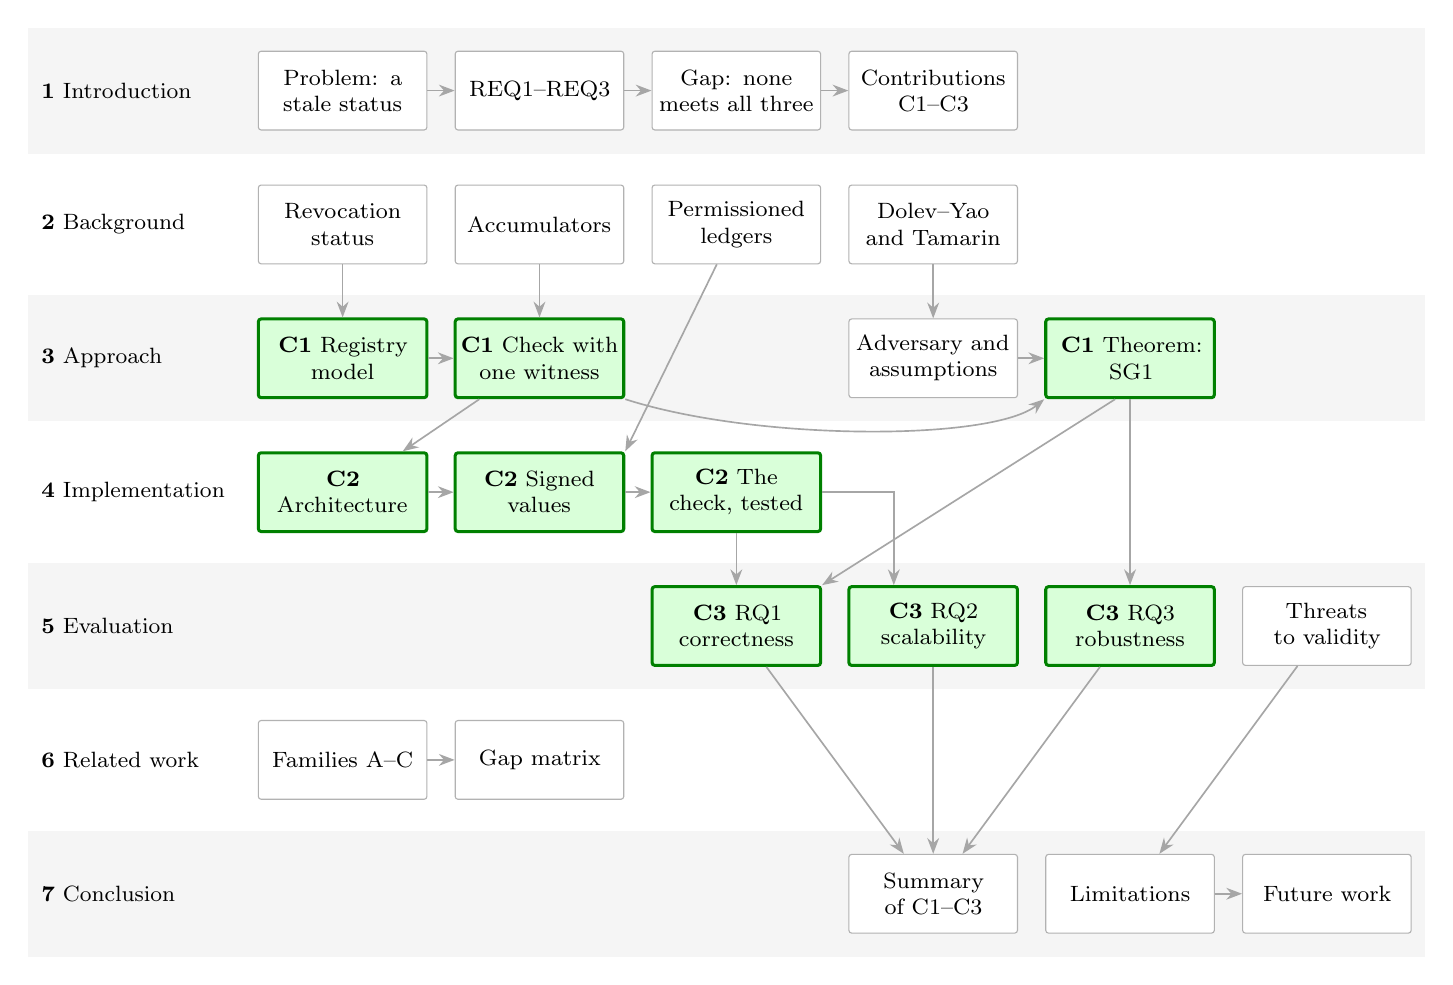
\begin{tikzpicture}[
      x=25mm, y=-17mm,
      para/.style={draw=gray!60, fill=white, rounded corners=1pt, text width=20mm, minimum height=10mm,
        align=center, font=\footnotesize, inner sep=2pt, execute at begin node={\hyphenpenalty=10000}},
      contrib/.style={para, draw=green!50!black, line width=1.1pt, fill=green!15},
      dep/.style={-Stealth, gray!70, semithick}]
    % One band per chapter, in reading order; within a band, paragraphs keep their order in the chapter.
    \begin{scope}[on background layer]
      \foreach \r/\chap in {0/Introduction, 1/Background, 2/Approach, 3/Implementation,
                            4/Evaluation, 5/Related work, 6/Conclusion} {
        \pgfmathsetmacro{\n}{int(\r+1)}
        \pgfmathparse{mod(\r,2) ? "white" : "gray!8"}
        \fill[\pgfmathresult] (-1.6,\r-0.47) rectangle (5.5,\r+0.47);
        \node[anchor=west, font=\footnotesize] at (-1.58,\r) {\textbf{\n}~\chap};
      }
    \end{scope}
    \node[para]    (problem)  at (0,0) {Problem: a stale status};
    \node[para]    (req)      at (1,0) {REQ1--REQ3};
    \node[para]    (gap)      at (2,0) {Gap: none meets all three};
    \node[para]    (claims)   at (3,0) {Contributions C1--C3};
    \node[para]    (cred)     at (0,1) {Revocation status};
    \node[para]    (acc)      at (1,1) {Accumulators};
    \node[para]    (ledger)   at (2,1) {Permissioned ledgers};
    \node[para]    (dy)       at (3,1) {Dolev--Yao and Tamarin};
    \node[contrib] (model)    at (0,2) {\textbf{C1} Registry model};
    \node[contrib] (check)    at (1,2) {\textbf{C1} Check with one witness};
    \node[para]    (threat)   at (3,2) {Adversary and assumptions};
    \node[contrib] (thm)      at (4,2) {\textbf{C1} Theorem: SG1};
    \node[contrib] (arch)     at (0,3) {\textbf{C2} Architecture};
    \node[contrib] (design)   at (1,3) {\textbf{C2} Signed values};
    \node[contrib] (code)     at (2,3) {\textbf{C2} The check, tested};
    \node[contrib] (rq1)      at (2,4) {\textbf{C3} RQ1 correctness};
    \node[contrib] (rq2)      at (3,4) {\textbf{C3} RQ2 scalability};
    \node[contrib] (rq3)      at (4,4) {\textbf{C3} RQ3 robustness};
    \node[para]    (validity) at (5,4) {Threats to validity};
    \node[para]    (families) at (0,5) {Families A--C};
    \node[para]    (matrix)   at (1,5) {Gap matrix};
    \node[para]    (summary)  at (3,6) {Summary of C1--C3};
    \node[para]    (limits)   at (4,6) {Limitations};
    \node[para]    (future)   at (5,6) {Future work};
    % An arrow points from a paragraph to the paragraph that needs it.
    \draw[dep] (problem) -- (req);
    \draw[dep] (req) -- (gap);
    \draw[dep] (gap) -- (claims);
    \draw[dep] (cred) -- (model);
    \draw[dep] (acc) -- (check);
    \draw[dep] (model) -- (check);
    \draw[dep] (dy) -- (threat);
    \draw[dep] (threat) -- (thm);
    \draw[dep] (check.south east) .. controls (2.1,2.62) and (3.3,2.62) .. (thm.south west);
    \draw[dep] (check) -- (arch);
    \draw[dep] (ledger) -- (design.north east);
    \draw[dep] (arch) -- (design);
    \draw[dep] (design) -- (code);
    \draw[dep] (thm.250) -- (rq1.north east);
    \draw[dep] (code) -- (rq1);
    \draw[dep] (code.east) -| ($(rq2.north)+(-0.2,0)$);
    \draw[dep] (thm) -- (rq3);
    \draw[dep] (families) -- (matrix);
    \draw[dep] (rq1) -- (summary);
    \draw[dep] (rq2) -- (summary);
    \draw[dep] (rq3) -- (summary);
    \draw[dep] (validity) -- (limits);
    \draw[dep] (limits) -- (future);
  \end{tikzpicture}
  \caption{The guide's running example as a dependency graph: each contribution stands on the background and leads to an evaluation question. One band per chapter in reading order, one box per paragraph in its order within the chapter, and an arrow from a paragraph to each paragraph that needs it. Green boxes deliver the contribution in their tag, white boxes are context, and every arrow runs to a later chapter or rightwards within one. It is the paper of \cref{fig:mindmap} with fewer boxes: the figure keeps the paragraphs that carry the argument, not all of them.}\label{fig:depgraph}
\end{figure}

It can take either of two places in the paper. As \tplref{fig:overview}, it suits a work whose contribution is a model, a tool and an evaluation spread over several chapters, which a problem-to-result picture would flatten into one box; the green has to read at a glance, so merge a chapter's paragraphs into its sections when there are many. As the figure of the structure paragraph at the end of the introduction (\cref{app:chapters:structure}), it replaces the list of chapters: the paragraph says what the bands, arrows and colours mean, and the figure shows the rest.

Drawing it also checks the skeleton before any prose exists. Every arrow should run down to a later chapter or right within one; an arrow pointing up or left is a paragraph that needs something the reader has not reached yet, so move one of the two, or say where the missing part comes. A green box with no path to an evaluation question is a contribution the paper claims but does not back. A background box that no arrow leaves is background the paper does not use. Draw only the arrows a reader needs to follow the argument: the figure shows where the contribution is, not every cross-reference.

\section{Figures}\label{app:writing:figures}
Every figure is vector. Draw the final version in TikZ, in the paper repository, so that it uses the paper's fonts, scales without loss, and can be fixed by anyone in the last week; \cref{app:latex} shows the TikZ and pgfplots setup of this template. Sketch in \href{https://www.drawio.com/}{draw.io} while the figure is still changing, then redraw it in TikZ once the spine is agreed. An exported PDF is the last resort, for a figure from another paper or a screenshot. Plots come from pgfplots reading the CSV that \texttt{just reproduce} writes, so a changed measurement changes the figure without anyone redrawing it. Every axis has a label with a unit, and nothing in a figure is smaller than 10\,pt in print.

\section{Captions}\label{app:writing:captions}
A caption is the figure's own paragraph, and a reader who reads only figures and captions should follow the paper. A caption explains the figure; it does not describe it. Its first sentence states what the figure shows as a claim. Then it puts that claim in context: which question it answers, what a reader needs to know to understand it, and why the result is what it is. Anything the reader could get from the axes and the legend does not belong in the caption; anything they could not, does: the concept being measured, the assumption behind the setup, the reason one curve bends. A diagram gets two or three sentences; a result figure gets as many as the explanation needs. Nature's captions are the model, for example those of \citet{guide:gulyas2015navigable}; \cref{fig:caption-example} is one in this template's style.

\begin{figure}[!ht]
  \centering
  \begin{tikzpicture}
    \begin{groupplot}[group style={group size=2 by 1, horizontal sep=1.6cm}, width=0.5\linewidth, height=5cm,
      xmode=log, log basis x=10, xlabel={Issuers in the registry}, grid=major, tick label style={font=\scriptsize}, label style={font=\footnotesize}, legend style={font=\scriptsize, at={(0.03,0.97)}, anchor=north west}]
      \nextgroupplot[ylabel={Median check latency [ms]}, ymode=log, title={(a)}, title style={font=\footnotesize}]
        \addplot+[mark=*, blue!70!black] coordinates {(10,31) (100,33) (1000,35) (10000,38)};
        \addplot+[mark=square*, gray] coordinates {(10,34) (100,61) (1000,310) (10000,2900)};
        \addplot[dashed, red!70!black] coordinates {(10,40) (10000,40)};
        \legend{this work, list-based baseline, one round trip}
      \nextgroupplot[ylabel={Registry size [MB]}, title={(b)}, title style={font=\footnotesize}, ymode=log]
        \addplot+[mark=*, blue!70!black] coordinates {(10,2) (100,12) (1000,110) (10000,1050)};
        \addplot+[mark=square*, gray] coordinates {(10,1) (100,3) (1000,21) (10000,190)};
    \end{groupplot}
  \end{tikzpicture}
  \caption{\textbf{Revocation checks stay within one network round trip up to 10\,000 issuers, while the list-based baseline grows linearly.} This is the scalability question, RQ2: a registry that serves a national ecosystem must answer a check without the verifier noticing. Our registry stays flat because a check reads one accumulator witness whatever the number of issuers, whereas the baseline scans the issuer's list. The price is the storage in panel (b), which grows with the number of credentials ever issued; the robustness analysis shows this stays under what a single server holds today. Medians over 10 runs with fresh issuer sets, on one 8-core VM in the BME cloud. (Illustrative numbers for the guide's running example.)}\label{fig:caption-example}
\end{figure}

\section{The abstract}\label{app:writing:abstract}
The abstract has a job before it has a structure: it must convince two readers that the paper is worth their time. The first is us, when you register the summary on the portal; the second is the committee that assigns the reviewers and, later, the reviewers themselves, who read it before anything else. Both have to come away believing that the topic is \textbf{relevant}, that solving it is \textbf{non-trivial}, that what you did is \textbf{novel}, and that it is \textbf{correct}: the same four things the review sheet scores (\cref{app:tdk:sheet}). Then follow \weblink{https://www.nature.com/documents/nature-summary-paragraph.pdf}{Nature's summary paragraph guide}; the abstract in this template already has its seven steps as placeholders.

\section{Style}
\begin{itemize}
  \item The Chicago School of Writing lectures: \href{https://www.youtube.com/watch?v=vtIzMaLkCaM}{part I}, \href{https://www.youtube.com/watch?v=aFwVf5a3pZM}{part II}, \href{https://www.youtube.com/watch?v=gphdfSwYMWU}{part III}.
  \item \href{https://www.youtube.com/watch?v=Unzc731iCUY}{MIT: How to Speak}, for the conference talk.
  \item Good examples: Leslie Lamport's papers, the Raft paper, and the figures and captions of \citet{guide:gulyas2015navigable}.
  \item For contrast, read the original Paxos and PBFT papers next to the Raft paper: all three carry great ideas, and the Raft paper was written so that its idea is the easy part.
\end{itemize}

\section{Disclose AI use}\label{app:writing:ai}
The faculty's \href{https://vik.bme.hu/page/1346/}{guidelines on the use of AI} set these rules, and this template follows them:
\begin{itemize}
  \item \textbf{Declare every use} in the faculty's declaration (\tplref{aidecl}, after the bibliography): which tool, for what, which parts of the paper, and how large a share. It is required for every thesis and cannot be waived; we require it for the TDK too.
  \item \textbf{Cite facts and conclusions from an AI answer} that were not in your prompt, like any other source, in the faculty's required MLA form: a one-sentence summary of the prompt, the model with its version, the company, the date, and a link to the conversation if possible. The faculty's example: \enquote{Examples of harm-reduction initiatives} prompt. ChatGPT-4o, OpenAI, February 10, 2025. \texttt{bib/references.bib} has a commented entry in this form.
\end{itemize}
\begin{itemize}
  \item \textbf{Keep the essential work your own.} The supervisor decides whether enough of the results are clearly yours, and a submission is not approved if AI use is disproportionately large or touches the essential parts. In the faculty's words: \enquote{If the task was to develop software and most of it was produced with generative AI, this is not acceptable}, while AI-supported software that serves your own algorithm, procedure or analysis is acceptable.
\end{itemize}
Verifying an AI answer is always your responsibility; an answer can never be a reference by itself. \Cref{app:code:ai} covers the tools.

%----------------------------------------------------------------------------
\chapter{Code, tools and AI}\label{app:code}
%----------------------------------------------------------------------------
\section{GitHub}\label{app:code:github}
Everything you make lives in GitHub, in the three repositories of \cref{app:start:access}: code and models, notes and drawings, artifacts such as PDFs and presentations, and the paper itself through the Overleaf sync. GitHub is also how the code reaches the reader: anonymously for double-blind review, through \href{https://anonymous.4open.science/}{Anonymous GitHub}, and permanently with a DOI, through Zenodo (\cref{app:zenodo}).

\paragraph{Repository layout.} One notes repository at the top level, with the paper and the code as submodules, so that notes, paper and code stay apart while one clone holds them all:
\begin{itemize}[noitemsep]
  \item notes repository: \texttt{README.md} linking the pieces; \texttt{notes/} for notes, drawings and consultation summaries; \texttt{slides/} for presentations;
  \begin{itemize}[noitemsep]
    \item \texttt{paper/}: submodule, the Overleaf-synced paper repository, with the TikZ sources of every figure in \texttt{figures/};
    \item \texttt{code/}: submodule, the code repository: the code in \texttt{src/} and \texttt{tests/}, the measurement scripts and their raw results in \texttt{experiments/}, and at the root \texttt{README.md}, \texttt{LICENSE}, \texttt{.zenodo.json}, \texttt{CITATION.cff}, the \texttt{justfile}, the \texttt{Dockerfile} and \texttt{.devcontainer/}.
  \end{itemize}
\end{itemize}
Zenodo archives the code repository on its own, so each release holds exactly the code and data behind the paper's results (\cref{app:zenodo}).

\paragraph{One command.} In the code repository, run the recurring commands (build, test, reproduce the measurements) through \href{https://github.com/casey/just}{just}, a command runner: one \texttt{justfile} lists them, and \texttt{just reproduce} regenerates every figure and table of the paper. Name the recipes after the paper: \texttt{just fig-scalability} makes \tplref{fig:scalability}, \texttt{just tab-robustness} makes \tplref{tab:robustness}, and \texttt{just reproduce} runs them all. \texttt{just reproduce --smoke} does the same on a reduced workload in minutes, and a GitHub Actions workflow runs it on every push, so the README's commands cannot rot unnoticed.

\section{The README}\label{app:code:readme}
There are two kinds of code repository, and two READMEs. A \emph{results} repository exists so that a reviewer can regenerate the paper's numbers; a \emph{tool} repository is meant to be used by others after the paper. Every TDK produces the first; some produce the second. The code template's \texttt{README.md} is the results README, with the sections of the tool README in a commented block below it: delete the block if you have results only, uncomment it if you built a tool.

\paragraph{The results README.} In this order:
\begin{enumerate}[noitemsep]
  \item What this is, in two sentences, with the paper's title and the concept DOI badge (\cref{app:zenodo}).
  \item The one command: \texttt{docker run \dots{} reproduce}, which regenerates every figure and table (\cref{app:code:docker}); then \texttt{just reproduce} for readers who cloned the repository and installed the dependencies, which are listed, pinned and as few as possible.
  \item The results map: a table with one row per figure and table of the paper: its number, the command that makes it, the output path, and the wall-clock time on stated hardware.
  \item What does not reproduce: anything that needs a secret, special hardware, a long run or is nondeterministic, with the seed policy and the expected variance. The section is required even when it says that everything reproduces with fixed seeds.
  \item The results tag: which Git tag and Zenodo version the paper's numbers came from (\cref{app:zenodo:versions}).
  \item How to cite, and the license.
\end{enumerate}

\paragraph{The tool README} adds, after the results sections: how to install it, how to use it on the user's own input with one worked example, how to contribute, and who maintains it. A tool repository also follows the conventions of the open-source foundations we work with, for example the \href{https://github.com/LF-Decentralized-Trust/lab-proposals/blob/main/README.md}{LF Decentralized Trust Labs}: an Apache 2.0 \texttt{LICENSE}, a Developer Certificate of Origin sign-off on every commit (\texttt{git commit -s}), a \texttt{MAINTAINERS.md}, and a \texttt{SECURITY.md} saying how to report a vulnerability. A tool that meets them can be proposed as a lab after the TDK.

\section{Docker}\label{app:code:docker}
The easiest thing a reviewer can do is \texttt{docker run}; a computer science reviewer without Docker is not the reader we are writing for. The code template has two images:
\begin{itemize}[noitemsep]
  \item The \textbf{runtime image}, built by the \texttt{Dockerfile} at the root, whose entry point is \texttt{just}: \texttt{docker run --rm -v \$PWD/out:/out ghcr.io/<you>/<repo> reproduce} regenerates every result into \texttt{out/}, and \texttt{\dots{} fig-scalability} regenerates one. The image pins every dependency, so the result does not depend on the reviewer's machine.
  \item The \textbf{development image}, described by \texttt{.devcontainer/devcontainer.json}: the toolchain, the language servers and the test runner, so that VS Code, GitHub Codespaces and the Docker development environment feature open the repository ready to work in, and so that we work in the same environment as you when we help.
\end{itemize}
A GitHub Actions workflow builds both on every push and publishes the runtime image to the GitHub Container Registry on every release, so the Zenodo version and the image carry the same tag. The README's first command points at the image of the results tag.

\section{Behaviour-driven tests}
For behaviour-driven development (BDD), write the expected behaviour as scenarios with \href{https://cucumber.io/}{Cucumber}; the scenarios then double as evaluation cases that a reviewer can read.

\section{AI tools}\label{app:code:ai}
\paragraph{Disclose.} AI use must be disclosed in the appropriate form in both the TDK paper and the thesis: the faculty's declaration (\tplref{aidecl}, after the bibliography) and citations for AI-generated facts (\cref{app:writing:ai}).

\paragraph{Keep every conversation.} Save every AI conversation about your work, and never use temporary or incognito chats for it. You will need them later: the AI declaration asks for the essential part of each prompt, citing an AI answer needs its date and a link, and decisions, arguments and text can be extracted from old conversations long after you have forgotten them. Most tools save them already; make sure yours do and that you do not delete them.
\begin{itemize}[noitemsep]
  \item Claude Code keeps every session as a transcript under \path{~/.claude/projects/}, one file per session; Codex keeps them under \path{~/.codex/sessions/}.
  \item ChatGPT and Claude on the web keep conversations in your account history; create a share link for any conversation you cite.
  \item Other tools: check where they store history, and export it regularly if they do not keep it.
\end{itemize}
These transcripts can contain everything you pasted in, so keep them out of public repositories.

\paragraph{Tools, as of October 2026.} Advice on AI tools goes stale within months; this is what we recommend now.
\begin{itemize}
  \item Use the strongest models, as they are the best for research; we prefer Claude Fable and ChatGPT Astra. Ask us if we can help you set up a subscription.
  \item Prefer an agentic harness working in your repository over a chat in the cloud: Claude Code or Codex, ideally with a good front end such as T3 Code, GitKraken Kepler or herdr. Working in a repository gives you the best features, and you \emph{need} version control when an AI edits your files.
  \item Plugins and skills: the Matt Pocock and poetato plugins for productivity; caveman, ponytail, squeez and TRON if you want to spare tokens. We highly recommend the \href{https://www.aihero.dev/skills-grill-me}{grill-me skill} (\href{https://claudemarketplaces.com/skills/mattpocock/skills/grill-me}{marketplace page}); see also \href{https://github.com/cursor/plugins/blob/main/pstack/skills/unslop/SKILL.md}{unslop} and \href{https://github.com/DietrichGebert/ponytail/blob/main/skills/ponytail/SKILL.md}{ponytail}.
  \item Do not overconstrain your model with excess instructions: bloated \texttt{AGENTS.md} files and memories degrade the performance of any model. Prefer skills with clear, broad descriptions of when to use them.
\end{itemize}

%----------------------------------------------------------------------------
\chapter{Archiving the code on Zenodo}\label{app:zenodo}
%----------------------------------------------------------------------------
A GitHub link can move, change or disappear; a reviewer checking \textbf{correctness} (criterion D/2) needs the exact code your results came from.
\href{https://zenodo.org/}{Zenodo}, run by CERN, archives a GitHub release permanently and gives it a DOI, so cite the archived release, not the repository.
These steps follow Zenodo's documentation as of September 2026; if the interface differs, the linked pages are authoritative.

\section{Prepare the repository}
\begin{enumerate}
  \item A \texttt{README.md} that says how to install the code and reproduce every measurement in \tplref{chap:evaluation}.
  \item A \texttt{LICENSE} file; ask your supervisor which license to use.
  \item A \texttt{.zenodo.json} file in the repository root (\cref{lst:zenodo-json}). Zenodo takes the record's title, authors, license and links from it (\href{https://help.zenodo.org/docs/github/describe-software/zenodo-json/}{format and example}). Check that it is valid JSON before releasing.
  \item If the repository has a \texttt{CITATION.cff}, keep its fields in line with \texttt{.zenodo.json}; Zenodo uses \texttt{.zenodo.json} when both exist.
\end{enumerate}

\begin{listing}[!ht]
\begin{minted}{json}
{
  "title": "TODO Artifact for: <thesis title>",
  "description": "Code and measurement scripts for the TDK paper <thesis title>.",
  "upload_type": "software",
  "version": "1.0.0",
  "publication_date": "2026-11-01",
  "license": "MIT",
  "creators": [
    { "name": "TODO Surname, Given name", "affiliation": "Budapest University of Technology and Economics", "orcid": "0000-0000-0000-0000" }
  ],
  "keywords": ["TODO"]
}
\end{minted}
\caption{A minimal \texttt{.zenodo.json}.}\label{lst:zenodo-json}
\end{listing}

\section{Publish the first release}
\begin{enumerate}
  \item Sign in to \href{https://zenodo.org/}{Zenodo} with the GitHub account that owns the repository. Open the profile menu, then \emph{GitHub}; click \emph{Sync now}, find the repository, and switch its toggle on (\href{https://help.zenodo.org/docs/github/enable-repository/}{enable a repository}).
  \item Commit the prepared files. On GitHub, open \emph{Releases}, then \emph{Draft a new release}: create a new tag such as \texttt{v1.0.0} on the commit your measurements used, add release notes, and publish.
  \item Back on Zenodo's GitHub page, open the repository and wait for processing. Open the new record and check its files and metadata; a failed release shows an \emph{Errors} section (\href{https://help.zenodo.org/docs/github/archive-software/github-upload/}{archive a release}).
\end{enumerate}
If the repository cannot be connected to Zenodo, upload a prepared archive instead: \emph{+}, then \emph{New upload}, fill in the metadata, \emph{Preview}, \emph{Publish} (\href{https://help.zenodo.org/docs/deposit/create-new-upload/}{upload instructions}).

\section{Cite it}
Each release gets its own \emph{version DOI}; the \emph{concept DOI} stands for all versions together (\href{https://support.zenodo.org/help/en-gb/1-upload-deposit/97-what-is-doi-versioning}{DOI versioning}).
\begin{itemize}
  \item In the paper, cite the \textbf{version DOI} of the release your results came from, as the \texttt{artifact} entry in \texttt{bib/references.bib} shows, and cite it in \tplref{chap:implementation}.
  \item In \texttt{README.md}, put the badge of the \textbf{concept DOI}, so it always leads to the newest version. The record page's DOI badge dialog gives the Markdown.
  \item Copy both DOIs from the Zenodo record; never guess a DOI by changing its number.
\end{itemize}

\section{Release a new version}
Fix the code, update \texttt{version} and \texttt{publication\_date} in \texttt{.zenodo.json}, commit, and publish a new GitHub release with a new tag (for example \texttt{v1.0.1}). Zenodo adds it to the same record as a new version with a new version DOI (\href{https://help.zenodo.org/docs/deposit/manage-versions/}{manage versions}). Never move an old tag. If the paper's results now come from the new version, cite its version DOI.

%----------------------------------------------------------------------------
\chapter{Glossary}\label{app:glossary}
%----------------------------------------------------------------------------
Three lists: the words we use about the process (\cref{tab:glossary-process}), technical terms from our topics (\cref{tab:glossary-technical}), and English--Hungarian pairs for writing the Hungarian abstract and talking about your work in Hungarian (\cref{tab:glossary-hu}).

\section{Process terms}
{\small
\begin{xltabular}{\linewidth}{>{\raggedright\arraybackslash}p{0.24\linewidth} X}
  \caption{Process terms.}\label{tab:glossary-process}\\
  \toprule \textbf{Term} & \textbf{Meaning} \\ \midrule \endfirsthead
  \toprule \textbf{Term} & \textbf{Meaning} \\ \midrule \endhead
  \bottomrule \endlastfoot
  Topic manifest & One page approved before the semester: the problem, why it matters, the expected contribution. \\
  Literature review (SLR) & A systematic literature review: searching sources with logged queries, screening them, and extracting what each says, so the gap claim rests on a known set of papers. \\
  Gap analysis & Finding what no existing approach does; ends in the gap matrix and a one-sentence gap. \\
  Gap matrix & The table of requirements against approaches in \tplref{chap:related}; the gap is the column where every row is met. \\
  Leading figure (vezérábra) & The one figure that explains the work; see \cref{app:writing:figure}. \\
  Spine & One page fixing the paper's claims, terminology and notation; see \cref{app:writing:spine}. \\
  Skeleton mind map & Every chapter as paragraph topic sentences with their evidence, before any prose. \\
  Beats & The moves inside each paragraph of the skeleton. \\
  Premortem & Imagining the paper has been rejected and writing the reviewer's reasons, to find fatal flaws before drafting. \\
  Anchor & A one-page artefact agreed with us that later work is measured against: the topic manifest, the spine, the full draft; see \cref{app:lifecycle}. \\
  Drift & Work that contradicts an anchor without re-opening it; see \cref{app:lifecycle}. \\
  Official step & A step of the faculty's TDK with a portal date: registration with the summary, paper upload, the conference; see \cref{app:tdk:dates}. \\
  Context upload & Putting our papers, notes and earlier work on the topic into \texttt{notes/} of your notes repository. \\
  Grind & A sustained push to close one large piece of work, such as all proofs or the full implementation. \\
  Review sheet hill climb & Scoring your own paper on the review sheet, fixing the weakest criterion, and repeating. \\
  Mirror principle & We put in what you put in, openly, and we value consistency over bursts; see \cref{app:consult}. \\
  Close with a summary & Saying back what was agreed at the end of a consultation, then posting it; see \cref{app:consult}. \\
  Last week's checklist & The polish phase as a list of checks, the mechanical half of them lint rules run by \texttt{make check} and the paper CI; see \cref{tab:polish}. \\
  Burn-down & The counts a draft drives to zero: todos, beats, placeholder figures, TODO cells; the paper CI records them on every push. \\
  Reviewer PDF & The paper built from \texttt{reviewer.tex}: no notes, no guide; the file to upload. \\
  Results tag & The Git tag and Zenodo version the paper's numbers came from; named in the paper and never moved; see \cref{app:zenodo}. \\
  Version DOI, concept DOI & The identifier of one archived release, and of all its versions together; the paper cites the concept DOI; see \cref{app:zenodo}. \\
\end{xltabular}
}

\section{Technical terms}
{\small
\begin{xltabular}{\linewidth}{>{\raggedright\arraybackslash}p{0.24\linewidth} X}
  \caption{Technical terms from our topics.}\label{tab:glossary-technical}\\
  \toprule \textbf{Term} & \textbf{Meaning} \\ \midrule \endfirsthead
  \toprule \textbf{Term} & \textbf{Meaning} \\ \midrule \endhead
  \bottomrule \endlastfoot
  Self-sovereign identity (SSI) & An identity model in which holders keep their own credentials and present them without asking the issuer each time. \\
  Verifiable credential (VC) & A digitally signed statement about a subject, issued by an issuer, held by a holder, and checked by a verifier (W3C standard). \\
  Verifiable data registry (VDR) & The shared registry that issuers, holders and verifiers trust for public data such as schemas, keys and revocation status. \\
  Zero-knowledge proof (ZKP) & A proof that a statement is true which reveals nothing beyond the statement itself. \\
  Hyperledger Fabric & A permissioned blockchain platform for consortia of known organisations. \\
  BPMN & Business Process Model and Notation, the standard notation for business process models. \\
  Tamarin & A prover for security protocols that searches for attacks under a symbolic adversary model. \\
  Lean & A proof assistant and programming language for machine-checked proofs. \\
  Refinery & A tool for partial modelling and graph generation over metamodels. \\
  Liveness, safety & A safety property says nothing bad ever happens; a liveness property says something good eventually happens. \\
  TOCTOU & Time-of-check to time-of-use: a race between checking a condition and acting on it. \\
\end{xltabular}
}
Each topic adds its own terms here; check the definitions against the topic's literature.

\section{English--Hungarian pairs}
Use one Hungarian term per concept and keep it throughout the Hungarian abstract and talk. The pairs below come from earlier TDK abstracts; where those used variants, the variant is listed too.
{\small
\begin{xltabular}{\linewidth}{>{\raggedright\arraybackslash}p{0.36\linewidth} >{\raggedright\arraybackslash}X}
  \caption{English--Hungarian pairs.}\label{tab:glossary-hu}\\
  \toprule \textbf{English} & \textbf{Hungarian} \\ \midrule \endfirsthead
  \toprule \textbf{English} & \textbf{Hungarian} \\ \midrule \endhead
  \bottomrule \endlastfoot
  Students' Scientific Conference & Tudományos Diákköri Konferencia (TDK) \\
  advisor & konzulens \\
  review sheet & bírálói lap \\
  leading figure & vezérábra \\
  abstract & kivonat, összefoglaló, rezümé \\
  appendix & függelék \\
  verifiable credential (VC) & ellenőrizhető tanúsítvány \\
  verifiable data registry (VDR) & ellenőrizhető adatregiszter (also: ellenőrizhető adatnyilvántartó) \\
  self-sovereign identity (SSI) & önrendelkező identitás (also: önrendelkezésű identitás) \\
  European Digital Identity Wallet (EUDIW) & Európai Digitális Identitástárca \\
  EU Business Wallet & EU üzleti tárca \\
  permissionless & engedélyhez nem kötött \\
  self-orchestrated & önszervező \\
  commitment & elköteleződés \\
  threshold-signed & küszöbaláírással ellátott \\
  race condition & versenyhelyzet \\
  check-then-act & ellenőrzést követő cselekvés \\
  liveness & elevenség \\
  adversary-driven & támadó-központú \\
  prover & bizonyító \\
  folding & hajtogatás \\
  timer event & időzítő esemény \\
  contrary-to-duty obligation & jóvátételi kötelezettség \\
  coordinated vulnerability disclosure (CVD) & koordinált sérülékenységközzététel \\
  zero-knowledge proof (ZKP) & nem-felfedő bizonyítás \\
\end{xltabular}
}
Where earlier papers used variants, the table gives the term we prefer.

%----------------------------------------------------------------------------
\chapter{Using this \LaTeX{} template}\label{app:latex}
%----------------------------------------------------------------------------
This chapter demonstrates the packages in \texttt{include/packages.tex}, theorem environments and tagged lists using one example: an issuer revoking verifiable credentials in a shared registry.
Copy examples from \texttt{guide/09-latex-template.tex}.
Put your packages and macros in \texttt{include/macros.tex}. \texttt{thesis.tex} loads it after the template preamble. Template updates preserve this file but replace the others under \texttt{include/}.
Use the existing theorem environments (\cref{app:latex:theorems}). A duplicate \texttt{\textbackslash newtheorem} with the same name stops the build.
\Cref{tab:package-index} lists all packages and links to their examples.

%----------------------------------------------------------------------------
\section{Todo notes (todonotes)}\label{app:latex:todo}
A margin note sits next to the line it refers to.\todo{A margin note.}
With 15\,mm margins, margin notes extend into the text edge to remain readable. Use inline notes for more than a few words:
\todo[inline]{An inline note: a block across the text width.}
\todoinline{The same, with the \texttt{\textbackslash todoinline} shortcut.}
\atodo[inline]{A longer review comment: \texttt{\textbackslash atodo} pre-fills the color and the author, and takes every \texttt{\textbackslash todo} option, here \texttt{inline}.}
\atodo[inline, author=IK, color=yellow!30]{The same with another author and color, given as options.}
\missingfigure{A placeholder for a figure that does not exist yet.}
\beat{what a paragraph establishes}{its evidence}{what the running example shows in it}{the next paragraph}
\advisortodo{A note for the advisors: a draft to confirm or a link to add.}
A margin comment from the supervisor.\atodo[nolist]{Cite this.}

Mark missing content in the sentence: proving one slice takes \tbd{the proving time} on a laptop; an unsupported claim needs a source\citeneeded[the 2023 survey]. These markers also work in table cells and captions, where margin notes cannot go (\cref{tab:latex:gaps}). Both appear in the todo list and disappear from the reviewer build. Use them instead of typed placeholder words or bracketed citation marks. The lint rejects typed markers and, at the final phase, any remaining \texttt{\textbackslash tbd} or \texttt{\textbackslash citeneeded}.
\begin{table}[!ht]
  \centering
  \caption{A table with a value still to measure, marked in its cell.}
  \label{tab:latex:gaps}
  \begin{tabular}{lrr}
    \toprule
    Proof & Cycles & Time \\
    \midrule
    real & 120\,000 & \tbd{after the runs} \\
    \bottomrule
  \end{tabular}
\end{table}
\begin{runningexample}[a box]
Set the example's name with \texttt{\textbackslash exname} in \texttt{thesis.tex}. If you use a custom example environment, name it in \texttt{\textbackslash lintexamplebox} so the lint checks that environment.
\end{runningexample}

The todo list follows the table of contents. Next comes the \emph{Checks} page, generated on each compile by the source lint (\cref{app:code:paperci}). The first page shows the phase and a mark for each essential (\cref{app:writing:essentials}) in reading order. It also groups essentials by chapter, marking those below the required level in red. The second page lists their next steps, other checks grouped by subject with initial findings, and counts. Failed checks also appear as \texttt{tdk-lint} package warnings in Overleaf's log.

Two lines in \texttt{thesis.tex} control the page. Set \texttt{\textbackslash lintphase} to \texttt{plan}, \texttt{draft}, \texttt{polish} or \texttt{final} as work progresses; checks become required when their phase is reached. Change \texttt{\textbackslash linttrue} to \texttt{\textbackslash lintfalse} to hide the page. To suppress a finding you have checked and rejected, add \texttt{\% lint-ignore: <rule> <reason>} on its line. A reason is required, and the page counts these suppressions.

Each finding says what is wrong and, under it, what to do: after an arrow, the text to write instead where the lint can work it out; otherwise, in italics, the instruction. A fix marked \emph{read it first} is most likely right but may change the meaning, and one with \texttt{<holes>} is a placeholder only you can fill. Overleaf cannot write fixes for you, so there you copy the text. In a local clone, \texttt{make fix} writes the safe fixes and prints what it changed, \texttt{make fix-dry} only prints them, and \texttt{make fix-review} also writes the ones to read first.
Build the submission from \texttt{reviewer.tex}. This four-line root sets the \texttt{final} class option, disables todonotes, defines \texttt{\textbackslash reviewermode} and inputs \texttt{thesis.tex}. The resulting PDF omits notes, the todo list and the guide. In Overleaf, open \texttt{reviewer.tex} and select \emph{Recompile from this file}; locally, run \texttt{make reviewer}. Inspect this PDF every week. It is the version reviewers will read.

%----------------------------------------------------------------------------
\section{Abbreviations, notation and terms (glossaries-extra)}\label{app:latex:acro}
Declare abbreviations, notation and terms in \texttt{content/glossary.tex}. The three tables after the acknowledgements contain only entries used in the text. Each use links to its table row.
\begin{itemize}[noitemsep]
  \item \textbf{Abbreviations.} First use expands the term: \glsreset{vc}\gls{vc}. Later uses are short: \gls{vc}. Use \glspl{vc} for the plural, or request a specific form with \glsxtrshort{zkp} and \glsxtrlong{zkp}. Declare it with \texttt{\textbackslash newabbreviation\{vc\}\{VC\}\{verifiable credential\}}.
  \item \textbf{Notation.} Declare each symbol once, with a description linking to its definition. For example, \gls{Rt} is the registry; $\gls{valid}$ also works in math. You may type \texttt{\$R\_t\$} directly elsewhere, but declare every symbol used in \cref{app:latex:theorems} and use \texttt{\textbackslash gls} at least when introducing it, so it enters the table.
  \item \textbf{Terms.} Define words with a fixed meaning in the paper: an \gls{issuer} signs, a \gls{holder} presents and a \gls{verifier} checks. Use \texttt{\textbackslash gls} on first use in each chapter to link back to the definition.
\end{itemize}
Use the template's \texttt{\textbackslash makenoidxglossaries} workflow. TeX sorts the lists, so no extra command is needed locally or on Overleaf. Give symbols a plain \texttt{sort} key. Do not mix in \texttt{makeglossaries} or \texttt{bib2gls}; they are unnecessary here and break this setup. Chapter one of the \texttt{glossaries-extra} user manual covers these features; see the \href{https://ctan.org/pkg/glossaries-extra}{package documentation}.

%----------------------------------------------------------------------------
\section{Citations, links and icons (natbib, hyperref, bookmark, orcidlink, fontawesome5)}\label{app:latex:cite}
The bibliography uses IEEE style through \texttt{tdkieee.bst}: entries are numbered by first citation, with abbreviated given names and IEEE punctuation. This meets the faculty's requirement for numbered references. Numeric citations are sorted and compressed~\cite{guide:w3c2025vcdm,guide:lamport1978time}.
\texttt{\textbackslash citet} names the author: \citet{guide:lamport1978time} introduced logical clocks.
\texttt{\textbackslash citep} brackets the reference~\citep{guide:lamport1978time}.

Links: \url{https://github.com/ftsrg} prints the address, \href{https://ftsrg.mit.bme.hu}{the research group} hides it.
The PDF bookmarks in the viewer's sidebar come from hyperref and bookmark.
Icons: \faGithub~source code, \faFilePdf~paper, \faEnvelope~contact. Author ORCID: \orcidlink{0000-0000-0000-0000}.

\paragraph{Quoting.} Put every verbatim quotation in \texttt{\textbackslash enquote} and follow it with a citation. Cite paraphrases too. Cite each borrowed result, concept, tool or product at first use, however familiar it is. Unmarked quotations count as plagiarism, and criterion B/2 also rewards proper citation.

\paragraph{Web pages.} The faculty guideline in \texttt{include/guideline.tex} requires: \enquote{Internetes hivatkozások megadásakor fontos, hogy az elérési út előtt megadjuk az oldal tulajdonosát és tartalmát (mivel a link egy idő után akár elérhetetlenné is válhat), valamint az elérés időpontját.} Use a \texttt{misc} entry. Set the author to the page owner in double braces, such as \texttt{author = \{\{W3C\}\}}, to keep its name intact. Give the page a descriptive title, a \texttt{url} and a \texttt{urldate} recording when you read it.

Zotero records the access date on saving and exports it as \texttt{urldate}. The template's \texttt{tdkieee.bst} prints it after the URL, for example \enquote{Accessed: 2026-10-25}; stock styles would omit it. Follow the \texttt{w3c2025vcdm} entry in \texttt{bib/references.bib}. The \texttt{bib} rule flags missing access dates. Use \cref{app:writing:refs} to decide whether a link belongs in the bibliography or a footnote.

\paragraph{Where the entries come from: Zotero.} Add sources to the group library with the browser's \href{https://www.zotero.org/download/connectors}{Zotero Connector}. Click it on the paper or DOI page, then correct the fetched metadata in Zotero so everyone gets the fix. Do not write literature entries by hand.

Overleaf's Zotero integration imports the group as \texttt{bib/zotero.bib} (\cref{app:start:access}). Use \emph{Refresh} to pull in additions. Zotero generates the citation keys; Overleaf suggests them when you type \texttt{\textbackslash cite\{}. For help, see the \href{https://www.zotero.org/support/quick_start_guide}{Zotero quick start guide}, \href{https://www.zotero.org/support/groups}{group libraries} and Overleaf's \href{https://www.overleaf.com/learn/how-to/How_to_link_your_Overleaf_account_to_Mendeley_and_Zotero}{linking your account to Zotero}. Locally, \href{https://retorque.re/zotero-better-bibtex/}{Better BibTeX} can keep an exported \texttt{.bib} in sync and provide stable citation keys.

When saving an entry, check its type and title capitalisation. Protect names and acronyms with braces, such as \texttt{\{BPMN\}}, and add a DOI if available. Keep hand-written Zenodo artifact and AI entries in \texttt{bib/references.bib}, because refresh overwrites \texttt{zotero.bib}.

%----------------------------------------------------------------------------
\section{Cross-references (cleveref)}\label{app:latex:cref}
Use \texttt{\textbackslash cref} for every cross-reference; it supplies the type name. Use \texttt{\textbackslash Cref} at the start of a sentence:
\cref{fig:latex:tikz,fig:latex:svg}, \cref{tab:latex:booktabs}, \cref{alg:latex:revoke}, \cref{lst:latex:verify}, \cref{eq:latex:window}, \cref{app:latex:theorems}.
Ranges compress: \cref{eq:latex:window,eq:latex:fresh,eq:latex:valid}.
\Cref{app:latex:theorems,app:latex:tags} reference every theorem-like environment and tagged list.
Label prefixes are listed in \texttt{include/preamble.tex}.

Chapter labels identify their role in the argument. The lint uses labels, not filenames: \texttt{ch:intro}, \texttt{ch:background}, \texttt{ch:approach}, \texttt{ch:implementation}, \texttt{ch:evaluation}, \texttt{ch:related} or \texttt{ch:conclusion}. Every numbered chapter needs a role. If a role spans several chapters, keep the plain label on the first and add a suffix to the others, such as \texttt{ch:approach:monitors}. A chapter serving two roles needs both labels, for example \texttt{ch:implementation} and \texttt{ch:evaluation}.

%----------------------------------------------------------------------------
\section{Mathematics and theorems (amsmath, unicode-math, ntheorem)}\label{app:latex:theorems}
A numbered equation:
\begin{equation}\label{eq:latex:window}
  \mathit{valid}(c, t) \iff t \in [t_\mathrm{issue}(c), t_\mathrm{exp}(c)) \land c \notin R_t .
\end{equation}
Aligned equations, each with its own number:
\begin{align}
  R_{t+1} &= R_t \cup \{ c \} \label{eq:latex:fresh}\\
  \mathit{valid}(c, t+1) &\implies \mathit{valid}(c, t) \label{eq:latex:valid}
\end{align}
Symbols beyond amsmath come from the math font: $\mathbb{N}$, $\mathcal{R}$, $\nexists$, $\varnothing$.

The following examples show every theorem environment in a typical order.
Definitions and examples have their own counters; the rest share the theorem counter.
\begin{definition}[Revocation registry]\label{def:latex:registry}
A \emph{revocation registry} is a set $R_t$ of revoked credential identifiers at time $t \in \mathbb{N}$.
\end{definition}
\begin{notation}\label{not:latex:issuer}
$I(c)$ denotes the issuer of credential $c$.
\end{notation}
\begin{example}\label{ex:latex:registry}
A university revokes a diploma credential $c$ at $t=5$, so $c \in R_5$.
\end{example}
\begin{invariant}\label{inv:latex:monotone}
The registry only grows: $R_t \subseteq R_{t+1}$ for every $t$.
\end{invariant}
\begin{property}[Revocation is final]\label{prty:latex:final}
If $c \in R_t$, then $\mathit{valid}(c, t')$ is false for every $t' \geq t$.
\end{property}
\begin{lemma}\label{lem:latex:step}
If $\mathit{valid}(c, t+1)$, then $\mathit{valid}(c, t)$, by \cref{eq:latex:valid}.
\end{lemma}
\begin{proof}
By \cref{inv:latex:monotone}, $c \notin R_{t+1}$ implies $c \notin R_t$.
\end{proof}
\begin{theorem}[Finality]\label{thm:latex:finality}
\Cref{prty:latex:final} holds for every registry that satisfies \cref{inv:latex:monotone}.
\end{theorem}
\begin{proof}
Induction on $t' - t$ with \cref{lem:latex:step}.
\end{proof}
\begin{corollary}\label{cor:latex:noresurrect}
A revoked credential is never valid again.
\end{corollary}
\begin{proposition}\label{prop:latex:size}
After $n$ revocations, $|R_t| = n$.
\end{proposition}
\begin{claim}\label{claim:latex:append}
An append-only log implements $R_t$.
\end{claim}
\begin{remark}\label{rem:latex:expiry}
Expiry is not revocation: an expired credential is not in $R_t$.
\end{remark}
References: \cref{def:latex:registry}, \cref{not:latex:issuer}, \cref{ex:latex:registry}, \cref{inv:latex:monotone}, \cref{prty:latex:final}, \cref{lem:latex:step}, \cref{thm:latex:finality}, \cref{cor:latex:noresurrect}, \cref{prop:latex:size}, \cref{claim:latex:append}, \cref{rem:latex:expiry}.

%----------------------------------------------------------------------------
\section{Tagged lists and other lists (enumitem)}\label{app:latex:tags}
Use tagged lists for stable names: C for contributions, REQ for requirements, DR for derived requirements, AS for assumptions, SG for guarantees, ADV for adversaries, LIM for limitations and RQ for research questions.
Each item starts with a short name in bold, and a gap-matrix row reuses its requirement's name.
A reference prints only the tag: \verb|\cref{asm:latex:clock}| prints \cref{asm:latex:clock}. Three or more consecutive tags become a range.
Add a new kind with one \texttt{\textbackslash NewTagList} line in \texttt{include/preamble.tex}.
\Cref{app:chapters} demonstrates all lists in their chapters: contributions and requirements in the introduction; threats, assumptions, guarantees and derived requirements in the approach; research questions in the evaluation; limitations in the conclusion. Here is one list with references:
\begin{assumptions}
  \item\label{asm:latex:clock} \textbf{Bounded drift.} Participants' clocks drift by at most $\delta$.
  \item\label{asm:latex:sig} \textbf{Unforgeable signatures.} The issuer's signature scheme is unforgeable.
  \item\label{asm:latex:ledger} \textbf{Ledger integrity.} Committed ledger history does not change.
\end{assumptions}
For items in a table, \verb|\tagrow{guarantees}| assigns the next list tag to a row. Add a label to reference it:
\begin{center}
\begin{tabular}{@{}lll@{}}
  \toprule
  & \textbf{Claim} & \textbf{Relies on} \\
  \midrule
  \tagrow{guarantees}\label{g:latex:monotone} & Monotone growth & \cref{asm:latex:ledger} \\
  \bottomrule
\end{tabular}
\end{center}
References: \cref{asm:latex:clock}, \cref{asm:latex:clock,asm:latex:sig}, \cref{asm:latex:clock,asm:latex:sig,asm:latex:ledger}, \cref{g:latex:monotone}.

Inline lists: the protocol has three roles, \begin{enumerate*}[label=(\roman*)] \item issuer, \item holder, and \item verifier. \end{enumerate*}
Compact lists:
\begin{itemize}[noitemsep]
  \item no extra space between items,
  \item set per list with enumitem options.
\end{itemize}

%----------------------------------------------------------------------------
\section{Figures (graphicx, svg, tikz, pgfplots, subcaption, wrapfig, rotating, placeins)}\label{app:latex:figures}
\Cref{fig:latex:tikz} is drawn in TikZ, so it uses the document's fonts and scales without blurring.
\begin{figure}[!ht]
  \centering
  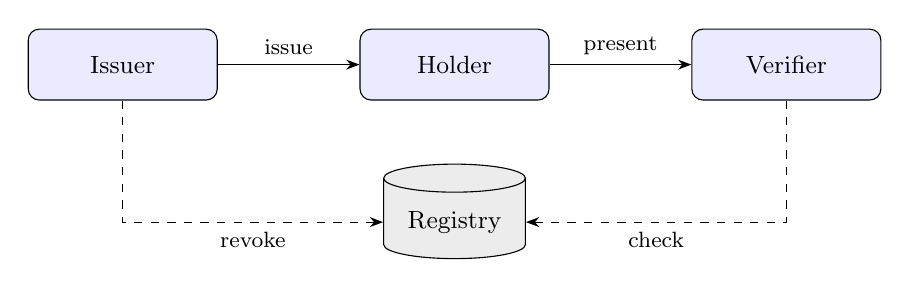
\begin{tikzpicture}[node distance=8mm and 18mm,
      role/.style={draw, rounded corners, fill=blue!8, minimum width=24mm, minimum height=9mm, font=\small},
      store/.style={draw, cylinder, shape border rotate=90, aspect=0.25, fill=gray!15, minimum width=18mm, minimum height=12mm, font=\small}]
    \node[role] (issuer) {Issuer};
    \node[role, right=of issuer] (holder) {Holder};
    \node[role, right=of holder] (verifier) {Verifier};
    \node[store, below=of holder] (reg) {Registry};
    \draw[-Stealth] (issuer) -- node[above, font=\footnotesize]{issue} (holder);
    \draw[-Stealth] (holder) -- node[above, font=\footnotesize]{present} (verifier);
    \draw[-Stealth, dashed] (issuer) |- node[pos=0.75, below, font=\footnotesize]{revoke} (reg);
    \draw[-Stealth, dashed] (verifier) |- node[pos=0.75, below, font=\footnotesize]{check} (reg);
  \end{tikzpicture}
  \caption{A TikZ diagram: roles and the revocation registry.}\label{fig:latex:tikz}
\end{figure}

\Cref{fig:latex:svg} is an SVG file included with \texttt{\textbackslash includesvg}. Overleaf converts it with Inkscape; local builds need \texttt{-shell-escape}.
Export draw.io and Inkscape drawings as SVG and include them this way, so the text stays sharp.
\begin{figure}[!ht]
  \centering
  \includesvg[width=0.35\linewidth]{guide/figures/example}
  \caption{An SVG figure.}\label{fig:latex:svg}
\end{figure}

\Cref{fig:latex:sub} places two subfigures side by side; each has its own label, \cref{fig:latex:sub-a} and \cref{fig:latex:sub-b}.
\begin{figure}[!ht]
  \centering
  \begin{subfigure}[b]{0.45\linewidth}
    \centering
    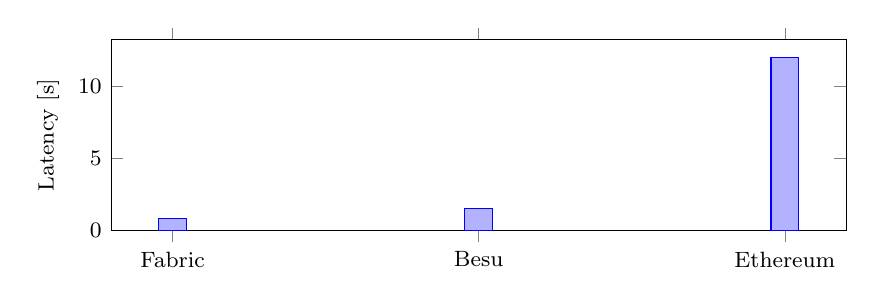
\begin{tikzpicture}
      \begin{axis}[ybar, width=0.9\linewidth, height=40mm, symbolic x coords={Fabric, Besu, Ethereum}, xtick=data, ylabel={Latency [s]}, ymin=0, font=\footnotesize]
        \addplot coordinates {(Fabric,0.8) (Besu,1.5) (Ethereum,12)};
      \end{axis}
    \end{tikzpicture}
    \caption{A pgfplots bar chart.}\label{fig:latex:sub-a}
  \end{subfigure}\hfill
  \begin{subfigure}[b]{0.45\linewidth}
    \centering
    
\includegraphics[width=0.6\linewidth]{figures/bme_logo}
    \caption{A PDF image via graphicx.}\label{fig:latex:sub-b}
  \end{subfigure}
  \caption{Subfigures with subcaption.}\label{fig:latex:sub}
\end{figure}

\begin{wrapfigure}{r}{0.3\linewidth}
  \centering
  \captionsetup{format=plain, justification=centering}
  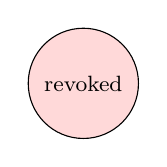
\begin{tikzpicture}
    \node[draw, circle, fill=red!15, minimum size=14mm, font=\footnotesize] {revoked};
  \end{tikzpicture}
  \caption{A wrapped figure.}\label{fig:latex:wrap}
\end{wrapfigure}
Text flows around \cref{fig:latex:wrap}, which wrapfig places at the right margin.
Use wrapfig only for small figures. Do not place it beside a list or section heading, where it breaks.
The paragraph needs enough lines to wrap around the figure, so this example continues for a few sentences.
A revoked credential stays revoked; the registry never forgets.
Verifiers check the registry before accepting a presentation.

\FloatBarrier
The \texttt{\textbackslash FloatBarrier} command from placeins, used above, prevents earlier figures from floating past it.
Use it before a section that must follow all earlier floats.

%----------------------------------------------------------------------------
\section{Colored boxes (tcolorbox)}\label{app:latex:boxes}
\begin{infobox}[Information]
  A general-purpose box for background facts.
\end{infobox}
\begin{warnbox}[Threat model caveat]
  A box for warnings and limitations.
\end{warnbox}
\begin{keybox}[Key insight]
  The \texttt{theo} style; any color works: \texttt{\textbackslash begin\{tcolorbox\}[theo=red, title=...]}.
\end{keybox}

%----------------------------------------------------------------------------
\section{Tables (booktabs, array, tabularx, xltabular, multirow, makecell, rotating)}\label{app:latex:tables}
\Cref{tab:latex:booktabs} demonstrates booktabs rules and array's \texttt{>\{\textbackslash bfseries\}} for a bold first column. It also uses a stretching tabularx column, multirow, makecell and an xcolor row.
\begin{table}[!ht]
  \centering
  \caption{A booktabs table with tabularx, multirow, makecell and a colored row.}\label{tab:latex:booktabs}
  \begin{tabularx}{\linewidth}{>{\bfseries}l X c}
    \toprule
    Platform & Revocation mechanism & \makecell{Latency\\{[s]}} \\
    \midrule
    \multirow{2}{*}{Fabric} & Chaincode-managed registry & 0.8 \\
     & Private data collections & 1.1 \\
    \rowcolor{gray!15}
    Ethereum & Smart-contract status list & 12 \\
    \bottomrule
  \end{tabularx}
\end{table}

\Cref{tab:latex:long} uses xltabular, which adds page breaks and repeated headers to tabularx.
\begin{xltabular}{\linewidth}{l X}
  \caption{A table that may break across pages.}\label{tab:latex:long}\\
  \toprule
  \textbf{Package} & \textbf{Purpose} \\
  \midrule
  \endfirsthead
  \toprule
  \textbf{Package} & \textbf{Purpose} \\
  \midrule
  \endhead
  todonotes & Visible notes while drafting \\
  acro & Acronyms expanded on first use \\
  tcolorbox & Colored boxes \\
  \bottomrule
\end{xltabular}

\Cref{tab:latex:sideways} uses rotating to put a wide table sideways on its own page.
\begin{sidewaystable}
  \centering
  \caption{A sideways table from rotating.}\label{tab:latex:sideways}
  \begin{tabular}{l c c c c c c}
    \toprule
    Approach & Offline check & Privacy & Finality & Open source & Throughput & Standardised \\
    \midrule
    Status list & \gapyes & -- & \gapyes & \gapyes & high & \gapyes \\
    Accumulator & \gapyes & \gapyes & \gapyes & \gappartial & medium & -- \\
    \bottomrule
  \end{tabular}
\end{sidewaystable}

%----------------------------------------------------------------------------
\section{Algorithms (algorithm, algpseudocode)}\label{app:latex:alg}
\begin{algorithm}[!ht]
  \caption{Revocation with a freshness check}\label{alg:latex:revoke}
  \begin{algorithmic}[1]
    \Require credential $c$, registry $R$, time $t$
    \If{$c \in R$}
      \State \Return \textsc{already-revoked}
    \EndIf
    \State $R \gets R \cup \{c\}$ \Comment{\cref{eq:latex:fresh}}
    \State \Return \textsc{ok}
  \end{algorithmic}
\end{algorithm}

%----------------------------------------------------------------------------
\section{Code with syntax highlighting (minted, listings)}\label{app:latex:code}
Use minted, with its Pygments highlighter, for common programming languages.
For a captioned listing, put a \texttt{minted} environment inside a \texttt{listing} float; in running text, use \mintinline{python}{print("inline")}.
Pygments supports over 500 languages. Find lexer names with \texttt{pygmentize -L lexers} or in the documentation's \href{https://pygments.org/docs/lexers/}{lexer list}.
Languages Pygments does not know (Refinery, Tamarin, Lean) go through listings with the styles in \texttt{include/code-languages.tex}: \lstinline[style=lean]{theorem le_succ (n : Nat) : n <= n + 1 := by omega}.
Inline listings must be ASCII under XeLaTeX; Unicode notation such as $\forall$ or $\mathbb{N}$ works in block listings (\cref{lst:latex:lean}).
Both are numbered as listings in one sequence, from \cref{lst:latex:refinery} to \cref{lst:latex:sql}.

\paragraph{Refinery, Tamarin and Lean (listings).}
\Cref{lst:latex:refinery,lst:latex:tamarin,lst:latex:lean} use the listings styles \texttt{refinery}, \texttt{tamarin} and \texttt{lean}.
\begin{lstlisting}[style=refinery, float=tbp, morekeywords={[2]Credential,Issuer,Holder}, caption={Refinery: a credential metamodel with an error predicate.}, label={lst:latex:refinery}]
class Issuer.
class Holder.
class Credential {
    Issuer[1] issuedBy
    Holder[1] heldBy
    contains Credential[0..1] revokes
}

pred selfRevoked(Credential c) <->
    revokes(c, c).

error unissued(Credential c) <->
    !issuedBy(c, _).
\end{lstlisting}

\begin{lstlisting}[style=tamarin, float=tbp, caption={Tamarin: revocation as a multiset-rewriting rule and a lemma.}, label={lst:latex:tamarin}]
theory Revocation
begin
builtins: signing

rule Revoke:
    [ !Issued($I, cred), Fr(~nonce) ]
  --[ Revoked(cred) ]->
    [ !RevokedFact(cred), Out(sign(<cred, ~nonce>, ~sk)) ]

lemma revoked_never_accepted:
  "All cred #i #j. Revoked(cred) @ i & Accepted(cred) @ j ==> j < i"
end
\end{lstlisting}

\begin{lstlisting}[style=lean, float=tbp, caption={Lean 4: the registry only grows (\cref{inv:latex:monotone}).}, label={lst:latex:lean}]
-- A registry is a list of revoked credential identifiers.
def Registry := List Nat

def revoke (r : Registry) (c : Nat) : Registry := c :: r

theorem revoke_monotone (r : Registry) (c x : Nat) :
    x ∈ r → x ∈ revoke r c := by
  intro h
  exact List.mem_cons_of_mem c h
\end{lstlisting}

\FloatBarrier
\paragraph{Common languages (minted).}
\Cref{lst:latex:verify} to \cref{lst:latex:sql} use the Pygments lexers \texttt{python}, \texttt{rust}, \texttt{go}, \texttt{java}, \texttt{typescript}, \texttt{solidity}, \texttt{json}, \texttt{yaml}, \texttt{bash} and \texttt{sql}.
\begin{listing}[!ht]
\begin{minted}{python}
def verify(credential, registry):
    # Reject revoked credentials before checking the signature.
    if credential.id in registry.revoked:
        return False
    return credential.signature_valid()
\end{minted}
\caption{Python.}\label{lst:latex:verify}
\end{listing}

\begin{listing}[!ht]
\begin{minted}{rust}
/// Appends a credential to the registry; revocation is final.
pub fn revoke(registry: &mut HashSet<CredentialId>, id: CredentialId) -> bool {
    registry.insert(id)
}
\end{minted}
\caption{Rust.}\label{lst:latex:rust}
\end{listing}

\begin{listing}[!ht]
\begin{minted}{go}
// IsRevoked reports whether the chaincode state marks the credential as revoked.
func (s *Registry) IsRevoked(ctx contractapi.TransactionContextInterface, id string) (bool, error) {
	v, err := ctx.GetStub().GetState("revoked/" + id)
	return v != nil, err
}
\end{minted}
\caption{Go (a Hyperledger Fabric chaincode function).}\label{lst:latex:go}
\end{listing}

\begin{listing}[!ht]
\begin{minted}{java}
public record Credential(String id, String issuer, Instant expires) {
    public boolean isValidAt(Instant t, Set<String> revoked) {
        return t.isBefore(expires) && !revoked.contains(id);
    }
}
\end{minted}
\caption{Java.}\label{lst:latex:java}
\end{listing}

\begin{listing}[!ht]
\begin{minted}{typescript}
interface StatusEntry { id: string; revoked: boolean }

export async function check(url: string, id: string): Promise<boolean> {
  const list: StatusEntry[] = await (await fetch(url)).json();
  return list.some((e) => e.id === id && e.revoked);
}
\end{minted}
\caption{TypeScript.}\label{lst:latex:ts}
\end{listing}

\begin{listing}[!ht]
\begin{minted}{solidity}
contract RevocationRegistry {
    mapping(bytes32 => bool) public revoked;
    event Revoked(bytes32 indexed id);

    function revoke(bytes32 id) external {
        require(!revoked[id], "already revoked");
        revoked[id] = true;
        emit Revoked(id);
    }
}
\end{minted}
\caption{Solidity.}\label{lst:latex:solidity}
\end{listing}

\FloatBarrier
\begin{listing}[!ht]
\begin{minted}{json}
{
  "@context": ["https://www.w3.org/ns/credentials/v2"],
  "type": ["VerifiableCredential"],
  "issuer": "did:example:university",
  "credentialStatus": { "type": "BitstringStatusListEntry", "statusListIndex": "94567" }
}
\end{minted}
\caption{JSON (a verifiable credential).}\label{lst:latex:json}
\end{listing}

\begin{listing}[!ht]
\begin{minted}{yaml}
# docker-compose.yml: one registry node for the measurements
services:
  registry:
    image: ghcr.io/example/registry:1.4
    ports: ["8080:8080"]
    environment:
      LOG_LEVEL: info
\end{minted}
\caption{YAML.}\label{lst:latex:yaml}
\end{listing}

\begin{listing}[!ht]
\begin{minted}{bash}
#!/usr/bin/env bash
# Run each benchmark size five times and collect the timings.
for n in 10 100 1000 10000; do
  for run in {1..5}; do
    ./bench --credentials "$n" >> "results/$n.csv"
  done
done
\end{minted}
\caption{Bash.}\label{lst:latex:bash}
\end{listing}

\begin{listing}[!ht]
\begin{minted}{sql}
-- Credentials revoked in the last day, per issuer.
SELECT issuer, COUNT(*) AS revoked
FROM revocations
WHERE revoked_at > NOW() - INTERVAL '1 day'
GROUP BY issuer
ORDER BY revoked DESC;
\end{minted}
\caption{SQL.}\label{lst:latex:sql}
\end{listing}
\FloatBarrier

%----------------------------------------------------------------------------
\section{Text (csquotes, ulem, xcolor, xspace, babel, setspace, lineno, comment)}\label{app:latex:text}
Quotes adapt to the language: \enquote{revocation is final}, and nested: \enquote{the issuer said \enquote{revoked}}.
ulem marks edits: \uline{underlined}, \sout{struck out}, \uwave{wavy}. xcolor colors text: \textcolor{red!70!black}{red}, \colorbox{yellow!40}{highlighted}.
Abbreviation macros use xspace, so they need no trailing braces: \eg the issuer, \ie the registry, Lamport \etal showed.
babel switches the hyphenation and quotes per phrase: \foreignlanguage{magyar}{\enquote{visszavont tanúsítvány}}.

\begin{onehalfspace}
setspace changes the line spacing for a block; this paragraph uses one-and-a-half spacing.
The rest of the thesis is single-spaced, as the TDK rules require.
\end{onehalfspace}

\begin{linenumbers}
lineno numbers lines, so reviewers can point at them.
Wrap a draft paragraph in a \texttt{linenumbers} environment, or put \texttt{\textbackslash linenumbers} in the preamble for the whole document.
\end{linenumbers}

The comment package hides source text without deleting it. The following \texttt{comment} block does not appear in the PDF.
\begin{comment}
This sentence is in the source but not in the PDF.
\end{comment}

%----------------------------------------------------------------------------
\section{Package index}\label{app:latex:index}
\newcommand{\ctan}[1]{\href{https://ctan.org/pkg/#1}{#1}}
\begin{xltabular}{\linewidth}{>{\ttfamily\raggedright\arraybackslash\hsize=1.1\hsize}X >{\raggedright\arraybackslash\hsize=0.9\hsize}X}
  \caption{Packages loaded by \texttt{include/packages.tex}, with links to examples and CTAN documentation. Open local documentation with \texttt{texdoc <name>}. See also \href{https://tikz.dev/}{tikz.dev} and the \href{https://pgfplots.sourceforge.net/}{pgfplots gallery}.}\label{tab:package-index}\\
  \toprule
  \normalfont\textbf{Package} & \textbf{Shown in} \\
  \midrule
  \endfirsthead
  \toprule
  \normalfont\textbf{Package} & \textbf{Shown in} \\
  \midrule
  \endhead
  \ctan{todonotes} & \cref{app:latex:todo} \\
  \ctan{glossaries-extra} & \cref{app:latex:acro}, and the three lists after the acknowledgements \\
  \ctan{natbib}, \ctan{hyperref}, \ctan{bookmark}, \ctan{orcidlink}, \ctan{fontawesome5} & \cref{app:latex:cite} \\
  \ctan{cleveref} & \cref{app:latex:cref}, and every reference in this chapter \\
  \ctan{amsmath}, \ctan{unicode-math} (\ctan{newtx} under pdfLaTeX), \ctan{ntheorem} & \cref{app:latex:theorems} \\
  \ctan{enumitem} & \cref{app:latex:tags} \\
  \ctan{graphicx}, \ctan{svg}, \ctan{tikz}, \ctan{pgfplots}, \ctan{subcaption}, \ctan{wrapfig}, \ctan{placeins} & \cref{app:latex:figures} \\
  \ctan{tcolorbox} & \cref{app:latex:boxes} \\
  \ctan{booktabs}, \ctan{array}, \ctan{tabularx}, \ctan{xltabular}, \ctan{multirow}, \ctan{makecell}, \ctan{rotating} & \cref{app:latex:tables} \\
  \ctan{algorithms}, \ctan{algorithmicx} & \cref{app:latex:alg} \\
  \ctan{listings}, \ctan{minted} & \cref{app:latex:code} \\
  \ctan{csquotes}, \ctan{ulem}, \ctan{xcolor}, \ctan{xspace}, \ctan{babel}, \ctan{setspace}, \ctan{lineno}, \ctan{comment} & \cref{app:latex:text} \\
  \ctan{caption} & Every caption: bold labels, hanging indent \\
  \ctan{anysize} & Page margins, set with \texttt{\textbackslash marginsize} in \texttt{thesis.tex} \\
  \ctan{microtype} & Character protrusion and font expansion on every page \\
  \ctan{emptypage} & Blank pages before chapters have no page number \\
  \ctan{ifxetex}, \ctan{ifluatex}, \ctan{fontspec}, \ctan{fontenc}, \ctan{inputenc}, \ctan{lm}, \ctan{newtx} & Text in TeX Gyre Termes (Times), code in Latin Modern Mono, under XeLaTeX, LuaLaTeX and pdfLaTeX \\
  \bottomrule
\end{xltabular}


\printacronyms

% The stock BME template guide, in Hungarian.
\selecthungarian
%----------------------------------------------------------------------------
\chapter{\LaTeX-eszközök}
\label{sec:LatexTools}
%----------------------------------------------------------------------------
\section{A szerkesztéshez használatos eszközök}
%----------------------------------------------------------------------------
Ez a sablon TeXstudio 2.8.8 szerkesztővel készült. A TeXstudio egy platformfüggetlen, Windows, Linux és Mac OS alatt is elérhető \LaTeX-szerkesztőprogram számtalan hasznos szolgáltatással (\refstruc{fig:TeXstudio}). A szoftver ingyenesen letölthető\footnote{A TeXstudio hivatalos oldala: \url{http://texstudio.sourceforge.net/}}.

\begin{figure}[!ht]
\centering
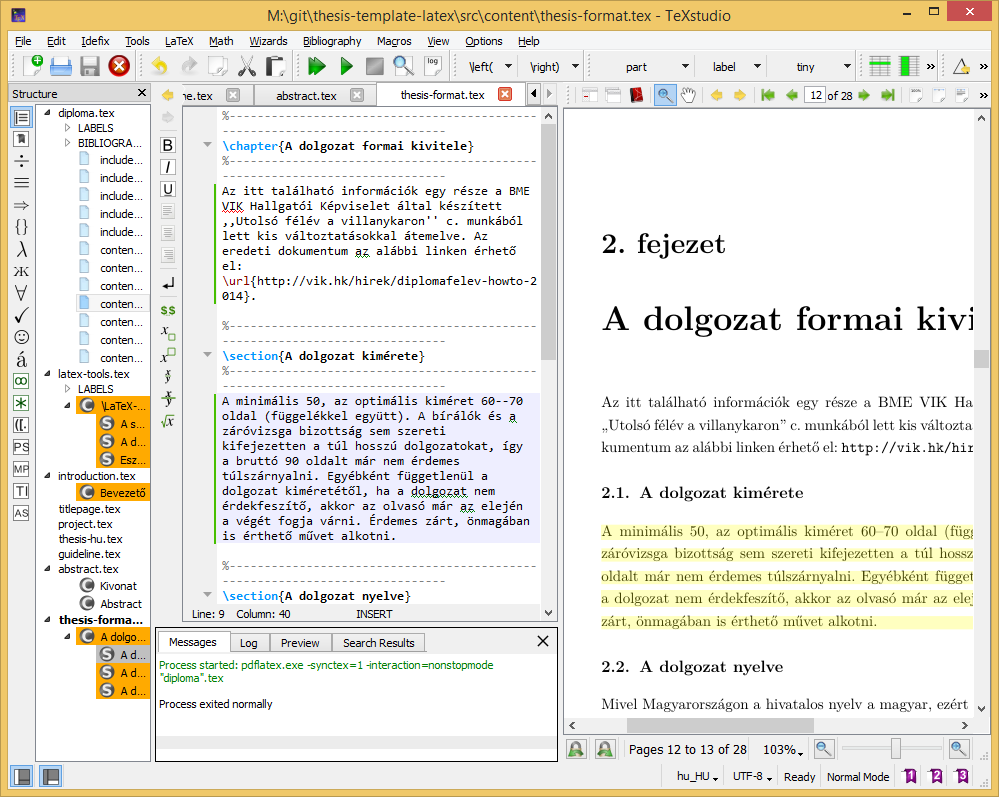
\includegraphics[width=150mm, keepaspectratio]{figures/TeXstudio.png}
\caption{A TeXstudio \LaTeX-szerkesztő.}
\label{fig:TeXstudio}
\end{figure}

A TeXstudio telepítése után érdemes még letölteni a magyar nyelvű helyesírásellenőrző-szótárakat hozzá. A TeXstudio az OpenOffice-hoz használatos formátumot tudja kezelni. A TeXstudio beállításainál a \verb+General+ fülön a \verb+Dictionaries+ résznél tudjuk megadni, hogy melyik szótárat használja.

Egy másik használható Windows alapú szerkesztőprogram a LEd\footnote{A LEd hivatalos oldala: \url{http://www.latexeditor.org/}} (LaTeX Editor), a TeXstudio azonban stabilabb, gyorsabb, és jobban használható.

%----------------------------------------------------------------------------
\section{A dokumentum lefordítása Windows alatt}
%----------------------------------------------------------------------------
A TeXstudio és a LEd kizárólag szerkesztőprogram (bár az utóbbiban DVI-nézegető is van), így a dokumentum fordításához szükséges eszközöket nem tartalmazza. Windows alatt alapvetően két lehetőség közül érdemes választani: MiKTeX (\url{http://miktex.org/}) és TeX Live (\url{http://www.tug.org/texlive/}) programcsomag. Az utóbbi működik Mac OS X, GNU/Linux alatt és Unix-származékokon is. A MiKTeX egy alapcsomag telepítése után mindig letölti a használt funkciókhoz szükséges, de lokálisan hiányzó \TeX-csomagokat, míg a TeX Live DVD ISO verzóban férhető hozzá. Ez a dokumentum TeX Live 2008 programcsomag segítségével fordult, amelynek DVD ISO verziója a megadott oldalról letölthető. A sablon lefordításához a disztribúcióban szereplő \verb+magyar.ldf+ fájlt a \verb+http://www.math.bme.hu/latex/+ változatra kell cserélni, vagy az utóbbi változatot be kell másolni a projekt-könyvtárba (ahogy ezt meg is tettük a sablonban) különben anomáliák tapasztalhatók a dokumentumban (pl. az ábra- és táblázat-aláírások formátuma nem a beállított lesz, vagy bizonyos oldalakon megjelenik alapértelmezésben egy fejléc). A TeX Live 2008-at még nem kell külön telepíteni a gépre, elegendő DVD-ről (vagy az ISO fájlból közvetlenül, pl. DaemonTools-szal) használni.

Ha a MiKTeX csomagot használjuk, akkor parancssorból a következő módon tudjuk újrafordítani a teljes dokumentumot:

\begin{lstlisting}[language=bash,frame=single,float=!ht]
$ texify -p thesis.tex
\end{lstlisting}

A \verb+texify+ parancs a MiKTex programcsomag \verb+miktex/bin+ alkönyvtárában található. A parancs gondoskodik arról, hogy a szükséges lépéseket (fordítás, hivatkozások generálása stb.) a megfelelő sorrendben elvégezze. A \verb+-p+ kapcsoló hatására PDF-et generál. A fordítást és az ideiglenes fájlok törlését elvégezhetjük a sablonhoz mellékelt \verb+manual_build.bat+ szkript segítségével is.

A \TeX-eszközöket tartalmazó programcsomag binárisainak elérési útját gyakran be kell állítani a szerkesztőprogramban, például TeXstudio esetén ezt legegyszerűbben az \emph{Options} menü \emph{Configure TeXstudio} pontjában, a \emph{Commands} lapon tehetjük meg.

A PDF-\LaTeX~használata esetén a generált dokumentum közvetlenül PDF-formátumban áll rendelkezésre. Amennyiben a PDF-fájl egy PDF-nézőben (pl. Adobe Acrobat Reader vagy Foxit PDF Reader) meg van nyitva, akkor a fájlleírót a PDF-néző program tipikusan lefoglalja. Ilyen esetben a dokumentum újrafordítása hibaüzenettel kilép. Ha bezárjuk és újra megnyitjuk a PDF dokumentumot, akkor pedig a PDF-nézők többsége az első oldalon nyitja meg a dokumentumot, nem a legutóbb olvasott oldalon. Ezzel szemben például az egyszerű és ingyenes \textcolor{blue}{Sumatra PDF} nevű program képes arra, hogy a megnyitott dokumentum megváltozását detektálja, és frissítse a nézetet az aktuális oldal megtartásával.

%----------------------------------------------------------------------------
\section{Eszközök Linuxhoz}
%----------------------------------------------------------------------------
Linux operációs rendszer alatt is rengeteg szerkesztőprogram van, pl. a KDE alapú Kile jól használható. Ez ingyenesen letölthető, vagy éppenséggel az adott Linux-disztribúció eleve tartalmazza, ahogyan a dokumentum fordításához szükséges csomagokat is. Az Ubuntu Linux disztribúciók alatt például legtöbbször a \verb+texlive-*+ csomagok telepítésével használhatók a \LaTeX-eszközök. A jelen sablon fordításához szükséges csomagok (kb. 0,5 GB) az alábbi paranccsal telepíthetők:

\begin{lstlisting}[language=bash,morekeywords={sudo,apt\-get},alsoletter={-},breaklines=true]
$ sudo apt-get install texlive-latex-extra texlive-fonts-extra texlive-fonts-recommended texlive-xetex texlive-science
\end{lstlisting}

Amennyiben egy újabb csomag hozzáadása után hiányzó fájlra utaló hibát kapunk a fordítótól, telepítenünk kell az azt tartalmazó TeX Live csomagot. Ha pl. a \verb+bibentry+ csomagot szeretnénk használni, futtassuk az alábbi parancsot:

\begin{lstlisting}[language=bash,morekeywords={apt\-cache},alsoletter={-},breaklines=true]
$ apt-cache search bibentry
texlive-luatex - TeX Live: LuaTeX packages
\end{lstlisting}

Majd telepítsük fel a megfelelő TeX Live csomagot, jelen esetben a `texlive-lualatex`-et. (Egy LaTeX csomag több TeX Live csomagban is szerepelhet.)

Ha gyakran szerkesztünk más \LaTeX dokumentumokat is, kényelmes és biztos megoldás a teljes TeX Live disztribúció telepítése, ez azonban kb. 4 GB helyet igényel.

\begin{lstlisting}[language=bash,morekeywords={sudo,apt\-get},alsoletter={-},breaklines=true]
sudo apt-get install texlive-full
\end{lstlisting}

%----------------------------------------------------------------------------
\chapter{A dolgozat formai kivitele}
%----------------------------------------------------------------------------
Az itt található információk egy része a BME VIK Hallgatói Képviselet által készített ,,Utolsó félév a villanykaron'' c. munkából lett kis változtatásokkal átemelve. Az eredeti dokumentum az alábbi linken érhető el: \url{http://vik.hk/hirek/diplomafelev-howto-2015}.

%----------------------------------------------------------------------------
\section{A dolgozat kimérete}
%----------------------------------------------------------------------------
Szakdolgozat esetében minimum 30, 45 körüli ajánlott oldalszám lehet az iránymutató. De mindenképp érdemes rákérdezni a konzulensnél is az elvárásokra, mert tanszékenként változóak lehetnek az elvárások.

Mesterképzésen a Diplomatervezés 1 esetében a beszámoló még inkább az Önálló laboratóriumi beszámolókhoz hasonlít, tanszékenként eltérő formai követelményekkel, -- egy legalább 30 oldal körüli dolgozat az elvárt -- és az elmúlt fél éves munkáról szól. De egyben célszerű, ha ez a végleges diplomaterv alapja is. (A végleges 60-90 oldal körülbelül a hasznos részre nézve)


%----------------------------------------------------------------------------
\section{A dolgozat nyelve}
%----------------------------------------------------------------------------
Mivel Magyarországon a hivatalos nyelv a magyar, ezért alapértelmezésben magyarul kell megírni a dolgozatot. Aki külföldi posztgraduális képzésben akar részt venni, nemzetközi szintű tudományos kutatást szeretne végezni, vagy multinacionális cégnél akar elhelyezkedni, annak célszerű angolul megírnia diplomadolgozatát. Mielőtt a hallgató az angol nyelvű verzió mellett dönt, erősen ajánlott mérlegelni, hogy ez mennyi többletmunkát fog a hallgatónak jelenteni fogalmazás és nyelvhelyesség terén, valamint -- nem utolsó sorban -- hogy ez mennyi többletmunkát fog jelenteni a konzulens illetve bíráló számára. Egy nehezen olvasható, netalán érthetetlen szöveg teher minden játékos számára.

%----------------------------------------------------------------------------
\section{A dokumentum nyomdatechnikai kivitele}
%----------------------------------------------------------------------------
A dolgozatot A4-es fehér lapra nyomtatva, 2,5 centiméteres margóval (+1~cm kötésbeni), 11--12 pontos betűmérettel, talpas betűtípussal és másfeles sorközzel célszerű elkészíteni.

Annak érdekében, hogy a dolgozat külsőleg is igényes munka benyomását keltse, érdemes figyelni az alapvető tipográfiai szabályok betartására~\cite{Jeney}.

% !TeX spellcheck = hu_HU
% !TeX encoding = UTF-8
% !TeX program = xelatex
%----------------------------------------------------------------------------
\chapter{A \LaTeX-sablon használata}
%----------------------------------------------------------------------------

Ebben a fejezetben röviden, implicit módon bemutatjuk a sablon használatának módját, ami azt jelenti, hogy sablon használata ennek a dokumentumnak a forráskódját tanulmányozva válik teljesen világossá. Amennyiben a szoftver-keretrendszer telepítve van, a sablon alkalmazása és a dolgozat szerkesztése \LaTeX-ben a sablon segítségével tapasztalataink szerint jóval hatékonyabb, mint egy WYSWYG (\emph{What You See is What You Get}) típusú szövegszerkesztő esetén (pl. Microsoft Word, OpenOffice).

%----------------------------------------------------------------------------
\section{Címkék és hivatkozások}
%----------------------------------------------------------------------------
A \LaTeX~dokumentumban címkéket (\verb+\label+) rendelhetünk ábrákhoz, táblázatokhoz, fejezetekhez, listákhoz, képletekhez stb. Ezekre a dokumentum bármely részében hivatkozhatunk, a hivatkozások automatikusan feloldásra kerülnek.

A sablonban makrókat definiáltunk a hivatkozások megkönnyítéséhez. Ennek megfelelően minden ábra (\emph{figure}) címkéje \verb+fig:+ kulcsszóval kezdődik, míg minden táblázat (\emph{table}), képlet (\emph{equation}), fejezet (\emph{section}) és lista (\emph{listing}) rendre a \verb+tab:+, \verb+eq:+, \verb+sec:+ és \verb+lst:+ kulcsszóval kezdődik, és a kulcsszavak után tetszőlegesen választott címke használható. Ha ezt a konvenciót betartjuk, akkor az előbbi objektumok számára rendre a \verb+\figref+, \verb+\tabref+, \verb+\eqref+, \verb+\sectref+ és \verb+\listref+ makrókkal hivatkozhatunk. A makrók paramétere a címke, amelyre hivatkozunk (a kulcsszó nélkül). Az összes említett hivatkozástípus, beleértve az \verb+\url+ kulcsszóval bevezetett web-hivatkozásokat is a  \verb+hyperref+\footnote{Segítségével a dokumentumban megjelenő hivatkozások nem csak dinamikussá válnak, de színezhetők is, bővebbet erről a csomag dokumentációjában találunk. Ez egyúttal egy példa lábjegyzet írására.} csomagnak köszönhetően aktívak a legtöbb PDF-nézegetőben, rájuk kattintva a dokumentum megfelelő oldalára ugrik a PDF-néző vagy a megfelelő linket megnyitja az alapértelmezett böngészővel. A \verb+hyperref+ csomag a kimeneti PDF-dokumentumba könyvjelzőket is készít a tartalomjegyzékből. Ez egy szintén aktív tartalomjegyzék, amelynek elemeire kattintva a nézegető behozza a kiválasztott fejezetet.

%----------------------------------------------------------------------------
\section{Ábrák és táblázatok}
%----------------------------------------------------------------------------
Használjunk vektorgrafikus ábrákat, ha van rá módunk. PDFLaTeX használata esetén PDF formátumú ábrákat lehet beilleszteni könnyen, az EPS (PostScript) vektorgrafikus képformátum beillesztését a PDFLaTeX közvetlenül nem támogatja (de lehet konvertálni, lásd később). Ha vektorgrafikus formában nem áll rendelkezésünkre az ábra, akkor a  veszteségmentes PNG, valamint a veszteséges JPEG formátumban érdemes elmenteni.  Figyeljünk arra, hogy ilyenkor a képek felbontása elég nagy legyen ahhoz, hogy nyomtatásban is megfelelő minőséget nyújtson (legalább 300 dpi javasolt). A dokumentumban felhasznált képfájlokat a dokumentum forrása mellett érdemes tartani, archiválni, mivel ezek hiányában a dokumentum nem fordul újra. Ha lehet, a vektorgrafikus képeket vektorgrafikus formátumban is érdemes elmenteni az újrafelhasználhatóság (az átszerkeszthetőség) érdekében.

Kapcsolási rajzok legtöbbször kimásolhatók egy vektorgrafikus programba (pl. CorelDraw) és onnan nagyobb felbontással raszterizálva kimenthatők PNG formátumban. Ugyanakkor kiváló ábrák készíthetők Microsoft Visio vagy hasonló program használatával is: Visio-ból az ábrák közvetlenül PDF-be is menthetők.

Lehetőségeink Matlab ábrák esetén:
\begin{itemize}
	\item Képernyőlopás (\emph{screenshot}) is elfogadható minőségű lehet a dokumentumban, de általában jobb felbontást is el lehet érni más módszerrel.
	\item A Matlab ábrát a \verb+File/Save As+ opcióval lementhetjük PNG formátumban (ugyanaz itt is érvényes, mint korábban, ezért nem javasoljuk).
	\item A Matlab ábrát az \verb+Edit/Copy figure+ opcióval kimásolhatjuk egy vektorgrafikus programba is és onnan nagyobb felbontással raszterizálva kimenthatjük PNG formátumban (nem javasolt).
	\item Javasolt megoldás: az ábrát a \verb+File/Save As+ opcióval EPS \emph{vektorgrafikus} formátumban elmentjük, PDF-be konvertálva beillesztjük a dolgozatba.
\end{itemize}
Az EPS kép az \verb+epstopdf+ programmal\footnote{a korábban említett \LaTeX-disztribúciókban megtalálható} konvertálható PDF formátumba. Célszerű egy batch-fájlt készíteni az összes EPS ábra lefordítására az alábbi módon (ez Windows alatt működik).
\begin{lstlisting}[language=]
@echo off
for %%j in (*.eps) do (
  echo converting file "%%j"
  epstopdf "%%j"
)
echo done .
\end{lstlisting}

Egy ilyen parancsfájlt (\verb+convert.cmd+) elhelyeztük a sablon \verb+figures\eps+ könyvtárába, így a felhasználónak csak annyi a dolga, hogy a \verb+figures\eps+ könyvtárba kimenti az EPS formátumú vektorgrafikus képet, majd lefuttatja a \verb+convert.cmd+ parancsfájlt, ami PDF-be konvertálja az EPS fájlt.

Ezek után a PDF-ábrát ugyanúgy lehet a dokumentumba beilleszteni, mint a PNG-t vagy a JPEG-et. A megoldás előnye, hogy a lefordított dokumentumban is vektorgrafikusan tárolódik az ábra, így a mérete jóval kisebb, mintha raszterizáltuk volna beillesztés előtt. Ez a módszer minden -- az EPS formátumot ismerő -- vektorgrafikus program (pl. CorelDraw) esetén is használható.

A képek beillesztésére \az+\refstruc{sec:LatexTools}ben mutattunk be példát (\refstruc{fig:TeXstudio}). Az előző mondatban egyúttal az automatikusan feloldódó ábrahivatkozásra is láthatunk példát. Több képfájlt is beilleszthetünk egyetlen ábrába. Az egyes képek közötti horizontális és vertikális margót metrikusan szabályozhatjuk (\refstruc{fig:HVSpaces}). Az ábrák elhelyezését számtalan tipográfiai szabály egyidejű teljesítésével a fordító maga végzi, a dokumentum írója csak preferenciáit jelezheti a fordító felé (olykor ez bosszúságot is okozhat, ilyenkor pl. a kép méretével lehet játszani).

\begin{figure}[!ht]
	\centering
	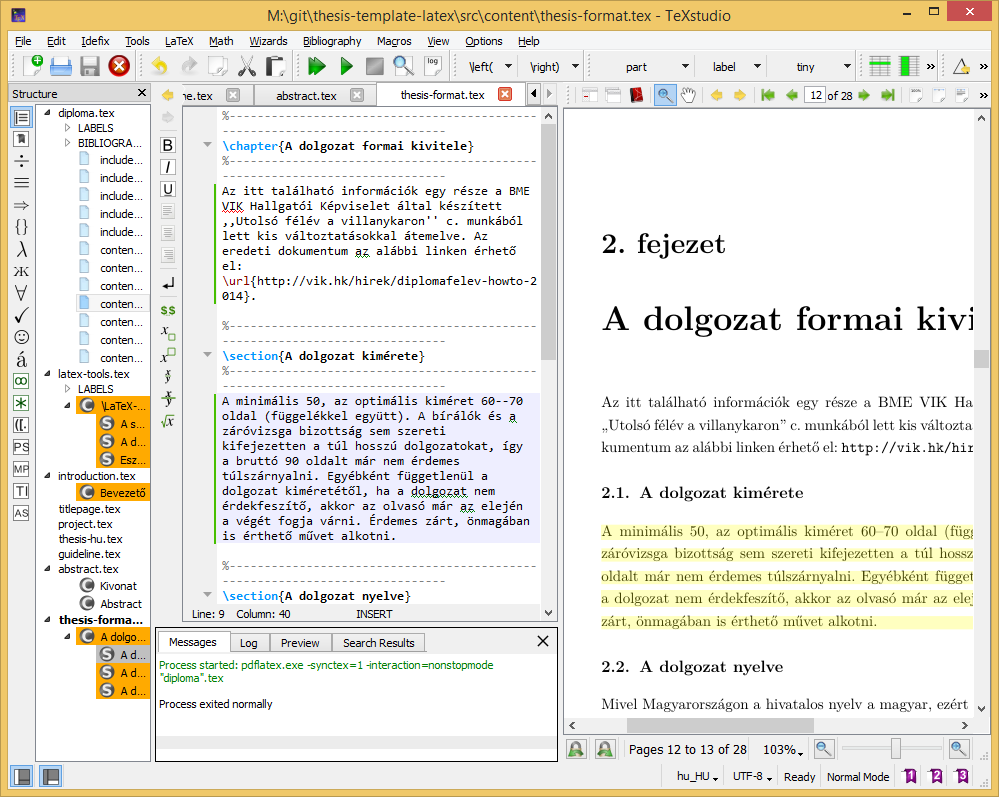
\includegraphics[width=67mm, keepaspectratio]{figures/TeXstudio.png}\hspace{1cm}
	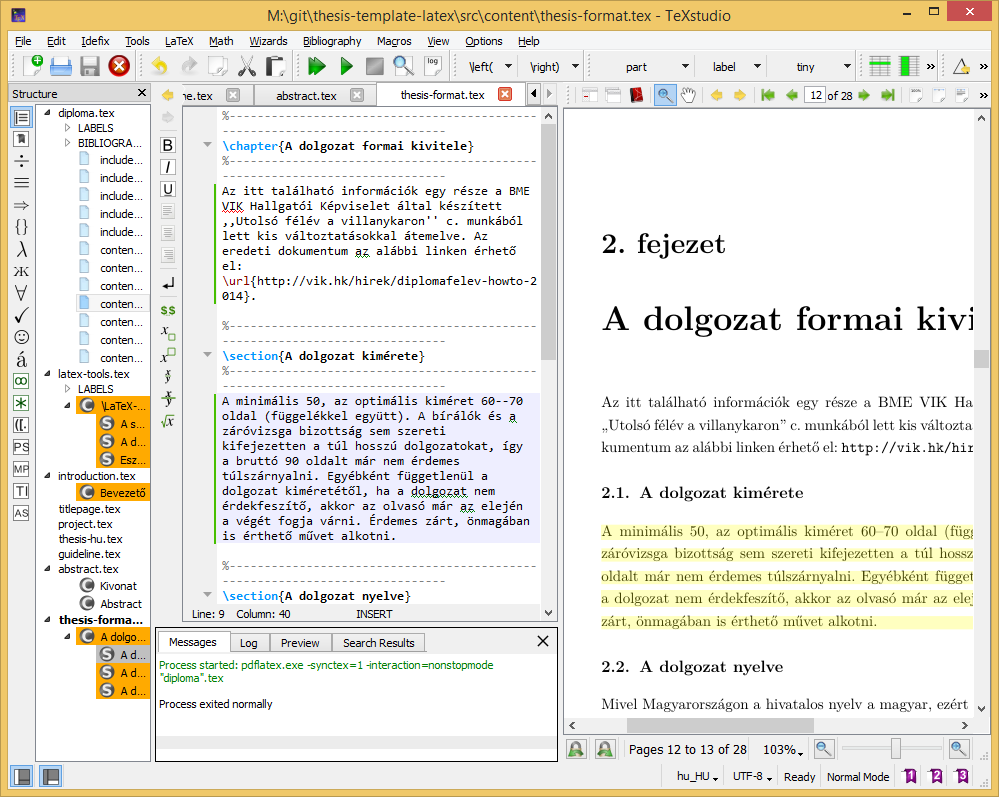
\includegraphics[width=67mm, keepaspectratio]{figures/TeXstudio.png}\\\vspace{5mm}
	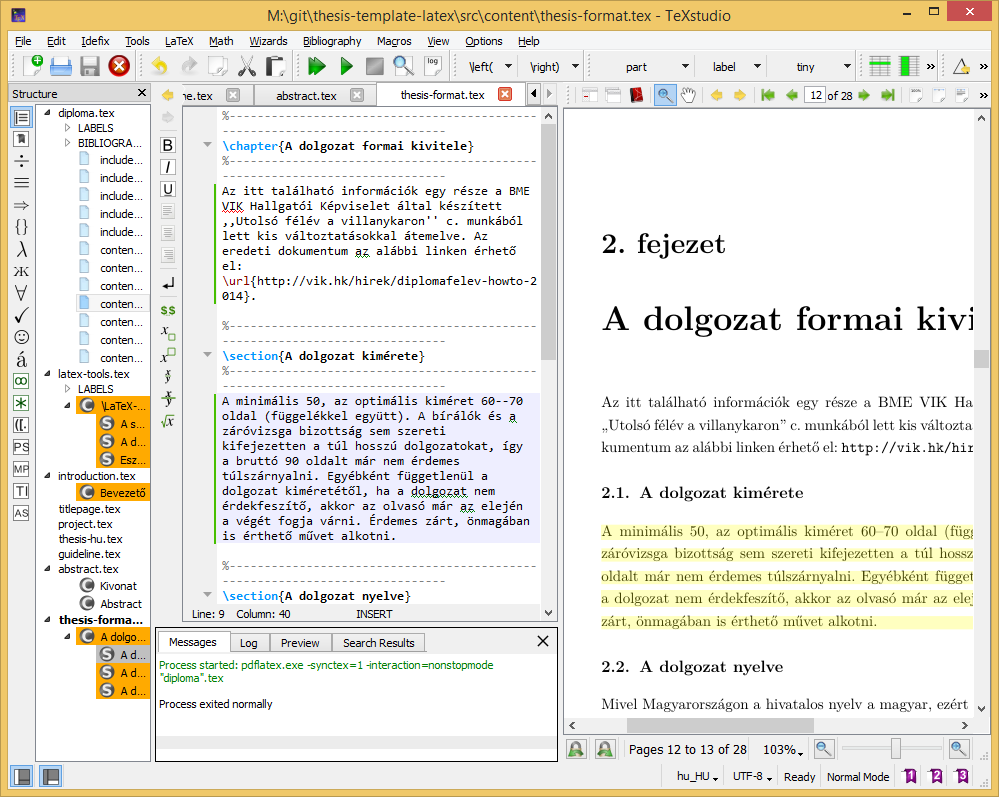
\includegraphics[width=67mm, keepaspectratio]{figures/TeXstudio.png}\hspace{1cm}
	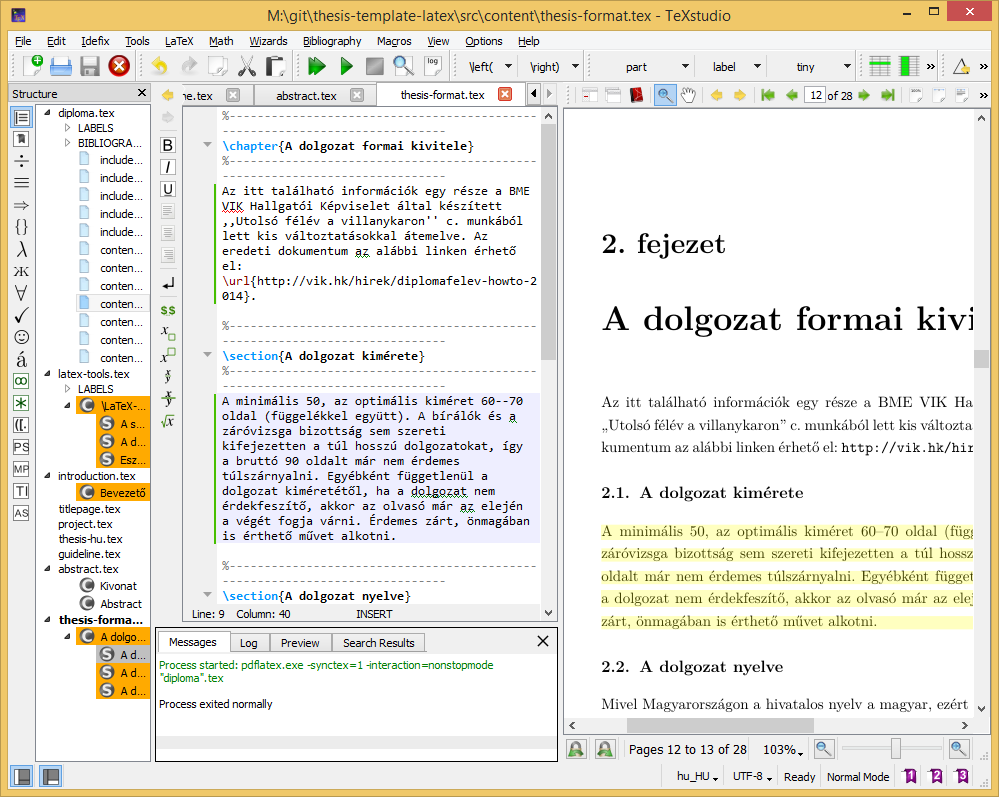
\includegraphics[width=67mm, keepaspectratio]{figures/TeXstudio.png}
	\caption{Több képfájl beillesztése esetén térközöket is érdemes használni.}
	\label{fig:HVSpaces}
\end{figure}

A táblázatok használatára \aref{tab:TabularExample}~táblázat mutat példát. A táblázatok formázásához hasznos tanácsokat találunk a \verb+booktabs+ csomag dokumentációjában.

\begin{table}[ht]
	\footnotesize
	\centering
	\begin{tabular}{ l c c }
		\toprule
		Órajel & Frekvencia & Cél pin \\
		\midrule
		CLKA & 100 MHz & FPGA CLK0\\
		CLKB & 48 MHz  & FPGA CLK1\\
		CLKC & 20 MHz  & Processzor\\
		CLKD & 25 MHz  & Ethernet chip \\
		CLKE & 72 MHz  & FPGA CLK2\\
		XBUF & 20 MHz  & FPGA CLK3\\
		\bottomrule
	\end{tabular}
	\caption{Az órajel-generátor chip órajel-kimenetei.}
	\label{tab:TabularExample}
\end{table}


%----------------------------------------------------------------------------
\section{Felsorolások és listák}
%----------------------------------------------------------------------------
Számozatlan felsorolásra mutat példát a jelenlegi bekezdés:
\begin{itemize}
	\item \emph{első bajusz:} ide lehetne írni az első elem kifejését,
	\item \emph{második bajusz:} ide lehetne írni a második elem kifejését,
	\item \emph{ez meg egy szakáll:} ide lehetne írni a harmadik elem kifejését.
\end{itemize}

Számozott felsorolást is készíthetünk az alábbi módon:
\begin{enumerate}
	\item \emph{első bajusz:} ide lehetne írni az első elem kifejését, és ez a kifejtés így néz ki, ha több sorosra sikeredik,
	\item \emph{második bajusz:} ide lehetne írni a második elem kifejését,
	\item \emph{ez meg egy szakáll:} ide lehetne írni a harmadik elem kifejését.
\end{enumerate}
A felsorolásokban sorok végén vessző, az utolsó sor végén pedig pont a szokásos írásjel. Ez alól kivételt képezhet, ha az egyes elemek több teljes mondatot tartalmaznak.

Listákban a dolgozat szövegétől elkülönítendő kódrészleteket, programsorokat, pszeudo-kódokat jeleníthetünk meg (\ref{lst:Example}.~kódrészlet).
\begin{lstlisting}[language=tex,caption=A fenti számozott felsorolás \LaTeX-forráskódja,label=lst:Example]
\begin{enumerate}
	\item \emph{els(*@ő@*) bajusz:} ide lehetne írni az els(*@ő@*) elem kifejését,
	és ez a kifejtés így néz ki, ha több sorosra sikeredik,
	\item \emph{második bajusz:} ide lehetne írni a második elem kifejését,
	\item \emph{ez meg egy szakáll:} ide lehetne írni a harmadik elem kifejését.
\end{enumerate}
\end{lstlisting}
A lista keretét, háttérszínét, egész stílusát megválaszthatjuk. Ráadásul különféle programnyelveket és a nyelveken belül kulcsszavakat is definiálhatunk, ha szükséges. Erről bővebbet a \verb+listings+ csomag hivatalos leírásában találhatunk.

%----------------------------------------------------------------------------
\section{Képletek}
%----------------------------------------------------------------------------
Ha egy formula nem túlságosan hosszú, és nem akarjuk hivatkozni a szövegből, mint például a $e^{i\pi}+1=0$ képlet, \emph{szövegközi képletként} szokás leírni. Csak, hogy másik példát is lássunk, az $U_i=-d\Phi/dt$ Faraday-törvény a $\rot E=-\frac{dB}{dt}$ differenciális alakban adott Maxwell-egyenlet felületre vett integráljából vezethető le. Látható, hogy a \LaTeX-fordító a sorközöket betartja, így a szöveg szedése esztétikus marad szövegközi képletek használata esetén is.

Képletek esetén az általános konvenció, hogy a kisbetűk skalárt, a kis félkövér betűk ($\mathbf{v}$) oszlopvektort -- és ennek megfelelően $\mathbf{v}^T$ sorvektort -- a kapitális félkövér betűk ($\mathbf{V}$) mátrixot jelölnek. Ha ettől el szeretnénk térni, akkor az alkalmazni kívánt jelölésmódot célszerű külön alfejezetben definiálni. Ennek megfelelően, amennyiben $\mathbf{y}$ jelöli a mérések vektorát, $\mathbf{\vartheta}$ a paraméterek vektorát és $\hat{\mathbf{y}}=\mathbf{X}\vartheta$ a paraméterekben lineáris modellt, akkor a \emph{Least-Squares} értelemben optimális paraméterbecslő $\hat{\mathbf{\vartheta}}_{LS}=(\mathbf{X}^T\mathbf{X})^{-1}\mathbf{X}^T\mathbf{y}$ lesz.

Emellett kiemelt, sorszámozott képleteket is megadhatunk, ennél az \verb+equation+ és a \verb+eqnarray+ környezetek helyett a korszerűbb \verb+align+ környezet alkalmazását javasoljuk (több okból, különféle problémák elkerülése végett, amelyekre most nem térünk ki). Tehát
\begin{align}
\dot{\mathbf{x}}&=\mathbf{A}\mathbf{x}+\mathbf{B}\mathbf{u},\\
\mathbf{y}&=\mathbf{C}\mathbf{x},
\end{align}
ahol $\mathbf{x}$ az állapotvektor, $\mathbf{y}$ a mérések vektora és $\mathbf{A}$, $\mathbf{B}$ és $\mathbf{C}$ a rendszert leíró paramétermátrixok. Figyeljük meg, hogy a két egyenletben az egyenlőségjelek egymáshoz igazítva jelennek meg, mivel a mindkettőt az \& karakter előzi meg a kódban. Lehetőség van számozatlan kiemelt képlet használatára is, például
\begin{align}
\dot{\mathbf{x}}&=\mathbf{A}\mathbf{x}+\mathbf{B}\mathbf{u},\nonumber\\
\mathbf{y}&=\mathbf{C}\mathbf{x}\nonumber.
\end{align}
Mátrixok felírására az $\mathbf{A}\mathbf{x}=\mathbf{b}$ inhomogén lineáris egyenlet részletes kifejtésével mutatunk példát:
\begin{align}
\begin{bmatrix}
a_{11} & a_{12} & \dots & a_{1n}\\
a_{21} & a_{22} & \dots & a_{2n}\\
\vdots & \vdots & \ddots & \vdots\\
a_{m1} & a_{m2} & \dots & a_{mn}
\end{bmatrix}
\begin{pmatrix}x_1\\x_2\\\vdots\\x_n\end{pmatrix}=
\begin{pmatrix}b_1\\b_2\\\vdots\\b_m\end{pmatrix}.
\end{align}
A \verb+\frac+ utasítás hatékonyságát egy általános másodfokú tag átviteli függvényén keresztül mutatjuk be, azaz
\begin{align}
W(s)=\frac{A}{1+2T\xi s+s^2T^2}.
\end{align}
A matematikai mód minden szimbólumának és képességének a bemutatására természetesen itt nincs lehetőség, de gyors referenciaként hatékonyan használhatók a következő linkek:\\
\indent\url{http://www.artofproblemsolving.com/LaTeX/AoPS_L_GuideSym.php},\\
\indent\url{http://www.ctan.org/tex-archive/info/symbols/comprehensive/symbols-a4.pdf},\\
\indent\url{ftp://ftp.ams.org/pub/tex/doc/amsmath/short-math-guide.pdf}.\\
Ez pedig itt egy magyarázat, hogy miért érdemes \verb+align+ környezetet használni:\\
\indent\url{http://texblog.net/latex-archive/maths/eqnarray-align-environment/}.

%----------------------------------------------------------------------------
\section{Irodalmi hivatkozások}
\label{sec:HowtoReference}
%----------------------------------------------------------------------------
Egy \LaTeX~dokumentumban az irodalmi hivatkozások definíciójának két módja van. Az egyik a \verb+\thebibliograhy+ környezet használata a dokumentum végén, az \verb+\end{document}+ lezárás előtt.
\begin{lstlisting}[language=tex]
\begin{thebibliography}{9}

\bibitem{Lamport94} Leslie Lamport, \emph{\LaTeX: A Document Preparation System}.
Addison Wesley, Massachusetts, 2nd Edition, 1994.

\end{thebibliography}
\end{lstlisting}

Ezek után a dokumentumban a \verb+\cite{Lamport94}+ utasítással hivatkozhatunk a forrásra. A fenti megadás viszonylag kötetlen, a szerző maga formázza az irodalomjegyzéket (ami gyakran inkonzisztens eredményhez vezet).

Egy sokkal professzionálisabb módszer a BiB\TeX{} használata, ezért ez a sablon is ezt támogatja. Ebben az esetben egy külön szöveges adatbázisban definiáljuk a forrásmunkákat, és egy külön stílusfájl határozza meg az irodalomjegyzék kinézetét. Ez, összhangban azzal, hogy külön formátumkonvenció határozza meg a folyóirat-, a könyv-, a konferenciacikk- stb. hivatkozások kinézetét az irodalomjegyzékben (a sablon használata esetén ezzel nem is kell foglalkoznia a hallgatónak, de az eredményt célszerű ellenőrizni). felhasznált hivatkozások adatbázisa egy \verb+.bib+ kiterjesztésű szöveges fájl, amelynek szerkezetét a \Aref{lst:Bibtex} kódrészlet demonstrálja. A forrásmunkák bevitelekor a sor végi vesszők külön figyelmet igényelnek, mert hiányuk a BiB\TeX-fordító hibaüzenetét eredményezi. A forrásmunkákat típus szerinti kulcsszó vezeti be (\verb+@book+ könyv, \verb+@inproceedings+ konferenciakiadványban megjelent cikk, \verb+@article+ folyóiratban megjelent cikk, \verb+@techreport+ valamelyik egyetem gondozásában megjelent műszaki tanulmány, \verb+@manual+ műszaki dokumentáció esetén stb.). Nemcsak a megjelenés stílusa, de a kötelezően megadandó mezők is típusról-típusra változnak. Egy jól használható referencia a \url{http://en.wikipedia.org/wiki/BibTeX} oldalon található.

\begin{lstlisting}[caption=Példa szöveges irodalomjegyzék-adatbázisra Bib\TeX{} használata esetén.,label=lst:Bibtex]
@book{Wettl04,
  author    = {Ferenc Wettl and Gyula Mayer and Péter Szabó},
  publisher = {Panem Könyvkiadó},
  title     = {\LaTeX~kézikönyv},
  year      = {2004},
}

@article{Candy86,
  author       = {James C. Candy},
  journaltitle = {{IEEE} Trans.\ on Communications},
  month        = {01},
  note         = {\doi{10.1109/TCOM.1986.1096432}},
  number       = {1},
  pages        = {72--76},
  title        = {Decimation for Sigma Delta Modulation},
  volume       = {34},
  year         = {1986},
}

@inproceedings{Lee87,
  author    = {Wai L. Lee and Charles G. Sodini},
  booktitle = {Proc.\ of the IEEE International Symposium on Circuits and Systems},
  location  = {Philadelphia, PA, USA},
  month     = {05~4--7},
  pages     = {459--462},
  title     = {A Topology for Higher Order Interpolative Coders},
  vol       = {2},
  year      = {1987},
}

@thesis{KissPhD,
  author      = {Peter Kiss},
  institution = {Technical University of Timi\c{s}oara, Romania},
  month       = {04},
  title       = {Adaptive Digital Compensation of Analog Circuit Imperfections for Cascaded Delta-Sigma Analog-to-Digital Converters},
  type        = {phdthesis},
  year        = {2000},
}

@manual{Schreier00,
  author       = {Richard Schreier},
  month        = {01},
  note         = {\url{http://www.mathworks.com/matlabcentral/fileexchange/}},
  organization = {Oregon State University},
  title        = {The Delta-Sigma Toolbox v5.2},
  year         = {2000},
}

@misc{DipPortal,
  author       = {{Budapesti Műszaki és Gazdaságtudományi Egyetem Villamosmérnöki és Informatikai Kar}},
  howpublished = {\url{http://diplomaterv.vik.bme.hu/}},
  title        = {Diplomaterv portál (2011. február 26.)},
}

@incollection{Mkrtychev:1997,
  author    = {Mkrtychev, Alexey},
  booktitle = {Logical Foundations of Computer Science},
  doi       = {10.1007/3-540-63045-7_27},
  editor    = {Adian, Sergei and Nerode, Anil},
  isbn      = {978-3-540-63045-6},
  pages     = {266-275},
  publisher = {Springer Berlin Heidelberg},
  series    = {Lecture Notes in Computer Science},
  title     = {Models for the logic of proofs},
  url       = {http://dx.doi.org/10.1007/3-540-63045-7_27},
  volume    = {1234},
  year      = {1997},
}
\end{lstlisting}

A stílusfájl egy \verb+.sty+ kiterjesztésű fájl, de ezzel lényegében nem kell foglalkozni, mert vannak beépített stílusok, amelyek jól használhatók. Ez a sablon a BiB\TeX-et használja, a hozzá tartozó adatbázisfájl a \verb+mybib.bib+ fájl. Megfigyelhető, hogy az irodalomjegyzéket a dokumentum végére (a \verb+\end{document}+ utasítás elé) beillesztett \verb+\bibliography{mybib}+ utasítással hozhatjuk létre, a stílusát pedig ugyanitt a  \verb+\bibliographystyle{plain}+ utasítással adhatjuk meg. Ebben az esetben a \verb+plain+ előre definiált stílust használjuk (a sablonban is ezt állítottuk be). A \verb+plain+ stíluson kívül természetesen számtalan más előre definiált stílus is létezik. Mivel a \verb+.bib+ adatbázisban ezeket megadtuk, a BiB\TeX-fordító is meg tudja különböztetni a szerzőt a címtől és a kiadótól, és ez alapján automatikusan generálódik az irodalomjegyzék a stílusfájl által meghatározott stílusban.

Az egyes forrásmunkákra a szövegből továbbra is a \verb+\cite+ paranccsal tudunk hivatkozni, így \aref{lst:Bibtex}.~kódrészlet esetén a hivatkozások a \verb+\cite+ parancs paraméterével rendre \texttt{Wettl04}, \texttt{Candy86}, \texttt{Lee87}, \texttt{KissPhD}, \texttt{Schreirer00}, \texttt{Mkrtychev:1997} és \texttt{DipPortal}. Az egyes forrásmunkák sorszáma az irodalomjegyzék bővítésekor változhat. Amennyiben az aktuális számhoz illeszkedő névelőt szeretnénk használni, használjuk az \verb+\acite{}+ parancsot.

Az irodalomjegyzékben alapértelmezésben csak azok a forrásmunkák jelennek meg, amelyekre található hivatkozás a szövegben, és ez így alapvetően helyes is, hiszen olyan forrásmunkákat nem illik az irodalomjegyzékbe írni, amelyekre nincs hivatkozás.

Mivel a fordítási folyamat során több lépésben oldódnak fel a szimbólumok, ezért gyakran többször is le kell fordítani a dokumentumot. Ilyenkor ez első 1-2 fordítás esetleg szimbólum-feloldásra vonatkozó figyelmeztető üzenettel zárul. Ha hibaüzenettel zárul bármelyik fordítás, akkor nincs értelme megismételni, hanem a hibát kell megkeresni. A \verb+.bib+ fájl megváltoztatáskor sokszor nincs hatása a változtatásnak azonnal, mivel nem mindig fut újra a BibTeX fordító. Ezért célszerű a változtatás után azt manuálisan is lefuttatni (TeXstudio esetén \verb+Tools/Bibliography+).

Hogy a szövegbe ágyazott hivatkozások kinézetét demonstráljuk, itt most sorban meghivatkozzuk a \cite{Wettl04}, \cite{Candy86}, \cite{Lee87}, \cite{KissPhD}, \cite{Schreier00} és \acite{Mkrtychev:1997}\footnote{Informatikai témában gyakran hivatkozunk cikkeket a Springer LNCS valamely kötetéből, ez a hivatkozás erre mutat egy helyes példát.} forrásmunkát, valamint \acite{DipPortal} weboldalt.

Megjegyzendő, hogy az ékezetes magyar betűket is tartalmazó \verb+.bib+ fájl az \verb+inputenc+ csomaggal betöltött \verb+latin2+ betűkészlet miatt fordítható. Ugyanez a \verb+.bib+ fájl hibaüzenettel fordul egy olyan dokumentumban, ami nem tartalmazza a \verb+\usepackage[latin2]{inputenc}+ sort. Speciális igény esetén az irodalmi adatbázis általánosabb érvényűvé tehető, ha az ékezetes betűket speciális latex karakterekkel helyettesítjük a \verb+.bib+ fájlban, pl. á helyett \verb+\'{a}+-t vagy ő helyett \verb+\H{o}+-t írunk.

Irodalomhivatkozásokat célszerű először olyan szolgáltatásokban keresni, ahol jó minőségű bejegyzések találhatók (pl. ACM Digital Library,\footnote{\url{https://dl.acm.org/}} DBLP,\footnote{\url{http://dblp.uni-trier.de/}} IEEE Xplore,\footnote{\url{http://ieeexplore.ieee.org/}} SpringerLink\footnote{\url{https://link.springer.com/}}) és csak ezek után használni kevésbé válogatott forrásokat (pl. Google Scholar\footnote{\url{http://scholar.google.com/}}). A jó minőségű bejegyzéseket is érdemes megfelelően tisztítani.\footnote{\url{https://github.com/FTSRG/cheat-sheets/wiki/BibTeX-Fixing-entries-from-common-sources}} A sablon angol nyelvű változatában használt \texttt{plainnat} beállítás egyik sajátossága, hogy a cikkhez generált hivatkozás a cikk DOI-ját és URL-jét is tartalmazza, ami gyakran duplikátumhoz vezet -- érdemes tehát a DOI-kat tartalmazó URL mezőket törölni. 

%----------------------------------------------------------------------------
\section{A dolgozat szerkezete és a forrásfájlok}
%----------------------------------------------------------------------------
A diplomatervsablonban a TeX fájlok két alkönyvtárban helyezkednek el. Az \verb+include+ könyvtárban azok szerepelnek, amiket tipikusan nem kell szerkesztenünk, ezek a sablon részei (pl. címoldal). A \verb+content+ alkönyvtárban pedig a saját munkánkat helyezhetjük el. Itt érdemes az egyes fejezeteket külön \TeX{} állományokba rakni.

A diplomatervsablon (a kari irányelvek szerint) az alábbi fő fejezetekből áll:
\begin{enumerate}
	\item 1 oldalas \emph{tájékoztató} a szakdolgozat/diplomaterv szerkezetéről (\verb+include/guideline.tex+), ami a végső dolgozatból törlendő,
	\item \emph{feladatkiírás} (\verb+include/project.tex+), a dolgozat nyomtatott verzójában ennek a helyére kerül a tanszék által kiadott, a tanszékvezető által aláírt feladatkiírás, a dolgozat elektronikus verziójába pedig a feladatkiírás egyáltalán ne kerüljön bele, azt külön tölti fel a tanszék a diplomaterv-honlapra,
	\item \emph{címoldal} (\verb+include/titlepage.tex+),
	\item \emph{tartalomjegyzék} (\verb+thesis.tex+),
	\item a diplomatervező \emph{nyilatkozat}a az önálló munkáról (\verb+include/declaration.tex+),
	\item 1-2 oldalas tartalmi \emph{összefoglaló} magyarul és angolul, illetve elkészíthető még további nyelveken is (\verb+content/abstract.tex+),
	\item \emph{bevezetés}: a feladat értelmezése, a tervezés célja, a feladat indokoltsága, a diplomaterv felépítésének rövid összefoglalása (\verb+content/introduction.tex+),
	\item sorszámmal ellátott \emph{fejezetek}: a feladatkiírás pontosítása és részletes elemzése, előzmények (irodalomkutatás, hasonló alkotások), az ezekből levonható következtetések, a tervezés részletes leírása, a döntési lehetőségek értékelése és a választott megoldások indoklása, a megtervezett műszaki alkotás értékelése, kritikai elemzése, továbbfejlesztési lehetőségek,
	\item esetleges \emph{köszönetnyilvánítás}ok (\verb+content/acknowledgement.tex+),
	\item részletes és pontos \emph{irodalomjegyzék} (ez a sablon esetében automatikusan generálódik a \verb+thesis.tex+ fájlban elhelyezett \verb+\bibliography+ utasítás hatására, \az+\refstruc{sec:HowtoReference}ban leírtak szerint),
	\item \emph{függelékek} (\verb+content/appendices.tex+).
\end{enumerate}

A sablonban a fejezetek a \verb+thesis.tex+ fájlba vannak beillesztve \verb+\include+ utasítások segítségével. Lehetőség van arra, hogy csak az éppen szerkesztés alatt álló \verb+.tex+ fájlt fordítsuk le, ezzel lerövidítve a fordítási folyamatot. Ezt a lehetőséget az alábbi kódrészlet biztosítja a \verb+thesis.tex+ fájlban.
\begin{lstlisting}
\includeonly{
	guideline,%
	project,%
	titlepage,%
	declaration,%
	abstract,%
	introduction,%
	chapter1,%
	chapter2,%
	chapter3,%
	acknowledgement,%
	appendices,%
}
\end{lstlisting}

Ha az alábbi kódrészletben az egyes sorokat a \verb+%+ szimbólummal kikommentezzük, akkor a megfelelő \verb+.tex+ fájl nem fordul le. Az oldalszámok és a tartalomjegyék természetesen csak akkor billennek helyre, ha a teljes dokumentumot lefordítjuk.

%----------------------------------------------------------------------------
\newpage
\section{Alapadatok megadása}
%----------------------------------------------------------------------------
A diplomaterv alapadatait (cím, szerző, konzulens, konzulens titulusa) a \verb+thesis.tex+ fájlban lehet megadni.

%----------------------------------------------------------------------------
\section{Új fejezet írása}
%----------------------------------------------------------------------------
A főfejezetek külön \verb+content+ könyvtárban foglalnak helyet. A sablonhoz 3 fejezet készült. További főfejezeteket úgy hozhatunk létre, ha új \TeX~fájlt készítünk a fejezet számára, és a \verb+thesis.tex+ fájlban, a \verb+\include+ és \verb+\includeonly+ utasítások argumentumába felvesszük az új \verb+.tex+ fájl nevét.


%----------------------------------------------------------------------------
\section{Definíciók, tételek, példák}
%----------------------------------------------------------------------------

\begin{definition}[Fluxuskondenzátor térerőssége]
Lorem ipsum dolor sit amet, consectetur adipiscing elit, sed do eiusmod tempor incididunt ut labore et dolore magna aliqua. Ut enim ad minim veniam, quis nostrud exercitation ullamco laboris nisi ut aliquip ex ea commodo consequat.
\end{definition}

\begin{example}
Példa egy példára. Duis aute irure dolor in reprehenderit in voluptate velit esse cillum dolore eu fugiat nulla pariatur. Excepteur sint occaecat cupidatat non proident, sunt in culpa qui officia deserunt mollit anim id est laborum.
\end{example}

\begin{theorem}[Kovács tétele]
Duis aute irure dolor in reprehenderit in voluptate velit esse cillum dolore eu fugiat nulla pariatur. Excepteur sint occaecat cupidatat non proident, sunt in culpa qui officia deserunt mollit anim id est laborum.
\end{theorem}

%----------------------------------------------------------------------------
\chapter{Példák a BME-sablonból}
\section{A TeXstudio felülete}
%----------------------------------------------------------------------------
\begin{figure}[!ht]
\centering
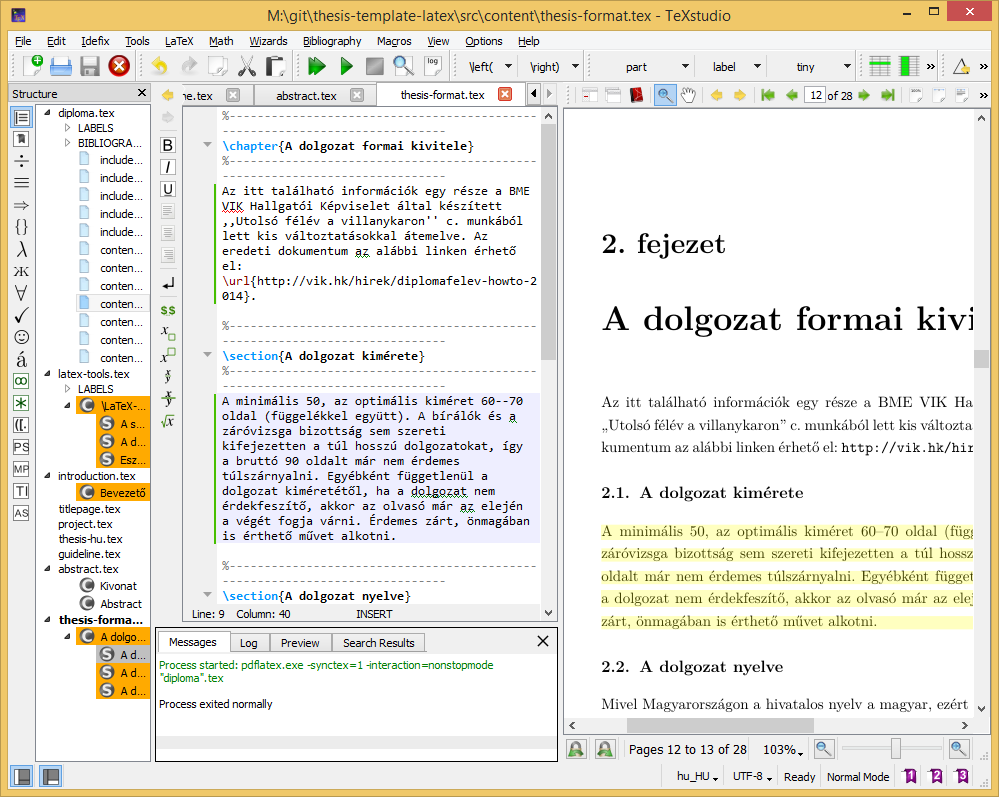
\includegraphics[width=150mm, keepaspectratio]{figures/TeXstudio.png}
\caption{A TeXstudio \LaTeX-szerkesztő.} 
\end{figure}

%----------------------------------------------------------------------------
\clearpage\section{Válasz az ,,Élet, a világmindenség, meg minden'' kérdésére}
%----------------------------------------------------------------------------
A Pitagorasz-tételből levezetve
\begin{align}
c^2=a^2+b^2=42.
\end{align}
A Faraday-indukciós törvényből levezetve
\begin{align}
\rot E=-\frac{dB}{dt}\hspace{1cm}\longrightarrow \hspace{1cm}
U_i=\oint\limits_\mathbf{L}{\mathbf{E}\mathbf{dl}}=-\frac{d}{dt}\int\limits_A{\mathbf{B}\mathbf{da}}=42.
\end{align}

\selectthesislanguage

\addcontentsline{toc}{chapter}{\bibname}
\bibliography{bib/references,bib/mybib}

\end{document}
